\documentclass{article}

\usepackage[utf8]{inputenc} % Use UTF-8 encoding
\usepackage{textgreek} % For Greek letters

\usepackage{float}
\usepackage{microtype}
\usepackage{xspace}
\bibliographystyle{plainurl}% the recommended bibstyle
\usepackage{placeins}

\usepackage{algorithm}% http://ctan.org/pkg/algorithms
\usepackage{algpseudocode}
\usepackage{hyperref}
\usepackage{fourier}
\usepackage{tikz}
\usetikzlibrary{decorations.pathreplacing}
\usetikzlibrary{patterns}
\usepackage{array}

\usepackage{mathtools}
\DeclarePairedDelimiter\ceil{\lceil}{\rceil}
\DeclarePairedDelimiter\floor{\lfloor}{\rfloor}

\DeclareMathAlphabet{\mathcal}{OMS}{cmsy}{m}{n}
\SetMathAlphabet{\mathcal}{bold}{OMS}{cmsy}{b}{n}

\newcommand{\bigO}{\mathcal{O}}
\newcommand{\cousize}{{\bf uint}\xspace}
\newcommand{\bs}{\ensuremath{B}\xspace}
\newcommand{\LineFor}[2]{%
	\State\algorithmicfor\ {#1}\ \algorithmicdo\ {#2} \algorithmicend\ \algorithmicfor%
}
\newcommand{\LineIf}[2]{%
	\State\algorithmicif\ {#1}\ \algorithmicthen\ {#2} \algorithmicend\ \algorithmicif%
}
\newcommand{\LineWhile}[2]{%
	\State\algorithmicwhile\ {#1}\ \algorithmicdo\ {#2} \algorithmicend\ \algorithmicwhile%
}

\newcommand{\pluseq}{\ensuremath{\mathrel{{+}\!\!\;{=}}}}
\newcommand{\minuseq}{\ensuremath{\mathrel{{-}\!\!\;{=}}}}
\newcommand{\plusplus}{\ensuremath{{+}\!\!\;{+}}}
\newcommand{\minusminus}{\ensuremath{{-}\!\!\;{-}}}

\newcommand\ips{\textsf{IPS$^4$o}}
\newcommand\blockqs{\textsf{BlockQS}}
\newcommand\stdsort{\textsf{stdsort}}
\newcommand\lomutoone{\textsf{BlockLomuto1}}
\newcommand\lomutotwo{\textsf{BlockLomuto2}}

\definecolor{gruen}{rgb}{0.95,0.95,0.95}
\definecolor{dunkelgruen}{rgb}{0.35, 0.7, 0.67}
\definecolor{hellgruen}{rgb}{0.84, 0.7, 0.39}

\newcommand{\gruen}{\color{gruen}}
\newcommand{\dunkelgruen}{\color{dunkelgruen}}
\newcommand{\hellgruen}{\color{hellgruen}}


\begin{document}

\section{Introduction}
Sorting algorithms on modern computers have been playing an important role in Computer Science and can date back to the early 50s and 60s. 
It is the great efforts that humans have put into the field of developing faster sorting algorithms that shapes the vital parts that formed
all the significant infrastructures of the vast computer world like databases, data centers, cluster networks etc.
In the realm of sorting algorithms, Quicksort, introduced by computer scientist Tony Hoare \cite{HoareQuickSort} to the public,
has made its way into the libc of the GNU/Linux system and stood the test of time as one of the most classical and widely used methods for sorting. 
Its divide-and-conquer strategy has been widely used and taken into research to fully utilize the performance of sorting.
The basic Quicksort picks an arbitrary pivot element,
partitions the array into 2 segments, one with elements less than the pivot and the other greater. 
It then recursively sorts these segments using the same method. While the original Quicksort method has proven effective,
the demand of further optimizations and the endless pursuit of efficiency has led to many variations to explore, one of which is the Multi-Pivot Quicksort. 

This thesis is my shallow attempt to unveil the benefits of Multi-Pivot Quicksort, exploring the effects more pivots can bring,
followed by some leveraged implementations of Multi-Pivot QuickSort and other variations alike and derived, analysis on the pros and cons that arise from multiple pivots.

\subsection{History and Related work}

When Quicksort was first brought to the fore a great number of variations and modifications were put into research over the years,
such as sorting with a better partition method and a more optimal strategy to select the arbitrary pivot element.
The innovative approach of Multi-pivot Quicksort bloomed, exemplified by Vladimir Yaroslavskiy \cite{Yaroslavskiy} in 2009,
Bentley and Bloch's algorithm (YBB Alogorithm), which was also highlighted by Wild and Nebel, adopted in Sun's Java 7 runtime library, 
introduces the use of two pivots. Contrary to initial expectations, studies have revealed that employing multiple pivots can enhance the performance,
challenging prior assumptions derived from the dual-pivot proposal by Sedgewick \cite{Sedgewick} in 1978 where he analyzed a dual-pivot approach, 
which was deemed inferior to the classical Quicksort in his research. Furthermore, Kushagra presented a 3-pivot Quicksort \cite{Kushagra} algorithm at ALENEX,
has attracted significant attention, further pushing the researches to broaden the boundaries of multi-pivot strategy. But how does it deal with the worst cases and how does it perform in practice? 

One common pitfall in the performance downgrade of the conventional Quicksort is the degenerated case,
which could often arise when the input array is already mostly sorted or when certain patterns in the data cause the algorithm to consistently choose poor pivots
that fail to split the data into evenly sized partitions. 
In such cases, the partitioning process may result in highly imbalanced partitions where the size of one partition is significantly larger than the other, leading to suboptimal performance and
potentially degrading the time complexity to $\bigO(n^2)$ instead of the expected $\bigO(n\log n)$ for Quicksort. This can be a serious issue when it comes to scalability on large datasets, thus
wiser choices of pivot selections could decrease the possiblities of such case from happening, such as the median-of-3 method and its variations of median-of-5 and median-of-7.
But on mostly ascending or descending arrays, whichever pivot we choose doesn't matter, the worst case is inevitable,
and it might not the best ideal approach to prevent the worst case from happening. Real world applications also bring concerns to us that duplicated elements are not rare,
and the median-of-n method could be easily affected by the duplicated elements, which could lead to the same worst case as the original Quicksort.
Of course we can set a threshold to set the minium length to use median-of-n method, but it doesn't fix the problem once and for all.
There are some other variations of Quicksort that have been proposed to address these specific issues, such as the Introsort algorithm \cite{Introsort} by David Musser,
which switches to Heapsort when the recursion depth exceeds a certain threshold. Thus the worst running time is guaranteed to be $\bigO(n\log n)$ by doing so.

And this is where Multi-pivot quicksort comes into play. Assuming we are dealing with randomly generated arrays,
since we don't know the exact size of each partition, the more pivots we choose, the more partitions we divide the array into,
the less chance it will be that we encounter imbalanced sizes of partitions. 
Moreover, choosing more pivots will significantly reduce the chance we access the same elements again and the maximum depth of recursion,
which can translate into better running time. With n pivots we are dividing the array into n+1 partitions, the same things happen on the sub-partitions 
in the next level of recursion and we can conclude the maximum depth of recursion would be $\log_{n+1} L$ given \textbf{n} as the number of pivots and \textbf{L} for the length of array.
Greater the n is, less the depth. Better memory behaviors can bring effects that can not be achieved by any of other traditional means such as choosing a better pivot value
among samples extracted from different parts of the array, but the drawbacks are also obvious, 
branch misprediction could be terrible as the different outcomes of comparisons can largely impact on the runtime performance.

\hypertarget{ref:BranchMisses}{}
\textit{This phenomenon was first observed by Kaligosi and Sanders (2006) on a Pentium 4 Prescott CPU, a processor with an extremely long pipeline, where the branch misprediction penalty was so high that a very skewed pivot choice outperformed the typically optimal median pivot, even though the latter leads to much fewer executed instructions in total.
The effect was not reproducible, however, on the slightly different Pentium 4 Willamette. Here two effects counteract: a biased pivot makes branches easier to predict but also gives unbalanced partition sizes. Brodal and Moruz have shown that this is a general trade-off in comparison-based sorting: One can only save comparisons at the price of additional branch misses.}
\cite{AnalysisOfBranchMissesInQuickSort}

This could also cause a delay of 14 to 19 stages on a typical Intel desktop CPU or 20 to 25 stages on AMD's Zen CPUs could lead to huge efficiency loss for our algorithm,
and this number only grows as the number of pivots increases and on more complicatad architectures. These are the trade-offs we have to consider when we are choosing the number of pivots,
although these side effects can be mitigated by the use of branchless comparisons and modern CPUs are able to run conditional move operations (CMOVE on x86) to avoid branches,
these overheads still remain as concerns, but it could relief the conflicting situations between total comparisons and the cost of branch mispredictions in some ways.
Apart from that, it could be really tricky when it comes to moving the elements to the right places among multiple partitions, especially when the number of pivots is large.
Additionally, comparisons are the second expensive things next to swaps we are dealing with, and the more pivots we choose, the more comparisons we have to make.
Even for the case of using only one pivot, the average number of comparisons remain unoptimial, being $1.38n\log n + \bigO(n)$ compared with the $n\log n + \bigO(n)$ of the Merge Sort,
but the overall instructions are much less than the average of Merge Sort and with proper pivot selection strategy, it can still be reduced to a certain extent.

% As the number of pivots increase, it is important that we take the worst cases into consideration. 
% Will we end up wasting too much time on comparing with badly-chosen similar pivots that split the array into imbalanced partitions,
% one of which might have much larger size than the rest? Or Even with the relatively higher amount of branch mispredictions, 
% will we still conquer the barriers of cache misses caused by long-lasting swaps of elements far away and reach a shorter time as the n grows?
% That's the riddle I'm going to research in the next section.

Fortunately, an efficient approach has been put forward by Stefan Edelkamp and Armin Weiß,
in their thesis of BlockQuickSort \cite{BlockQuickSort}
which evens the odds of both branch mis-prediction and cache misses which uses one or more buffer blocks of constant sizes on the stack
to store the index offsets of out-of-order elements, swap them altogether in a second pass to rearrange them in order
after scanning a large chunk of array with the size of the block.
It has eliminated almost all the $if$ branches during comparisons, except inevitable branches produced by terminating situation of $for$ loops which traverse the whole array.
Their approach realized a significant speedup up to 80\% faster compared with the GCC implementation of std sort
with only one single pivot. The BlockQuickSort has been adapted to the Multi-Pivot Quicksort and the results are also promising,
the improvements on contiguous memory access significantly improves the spatial locality and reduces both the cache misses and branch mis-predictions.
Branchless comparisons are also adapted which plays an important role in contributing to the huge performance boost by reducing the overhead
when increasing the counter of elements stored in the block buffer(s).
This novel approach has also developed variations that could effectively make the use of different partitioning methods and multiple pivots selected. 

Meanwhile, in the pursuit of advancing the efficiency of the Quicksort algorithm,
my investigation led me to explore various modifications, 
with a particular focus on the pattern-defeating Quicksort (PDQSort) proposed by Orson Peters. 
PDQSort leverages the average-case performance of randomized Quicksort with the rapid worst-case execution of heapsort, 
while concurrently achieving linear time complexity for slices exhibiting specific patterns. 
Notably, PDQSort employs a judicious application of randomization to prevent the degenerated case from happening.
When it does, PDQSort will strategically shuffle or reverse the entire array to simplify the sorting and potentially could increase the speed.
If all the counter measures fail, it also has the final backup plan of switching to Heapsort when bad choices of pivots or the depth of recursions exceed the limit,
learning the lesson from Introsort. 
In terms of pivot selection, it uses a fixed seed when generating a pseudo-random index to ensure the reproducibility and deterministic behavior.
Furthermore, in instances where randomly selected elements from the original array appear in a descending order.
The combination of these optimizations has demonstrated a significant enhancement in performance, showcasing PDQSort as up to twice faster than the original Quicksort algorithm. 
This outcome illuminates the transformative impact that a comprehensive analysis on the pattern of arrays has on the speed of sorting algorithms,
not to mention it is a successful combination of BlockQuickSort's partition method,
Heap sort when dealing with worst cases and Insertion sort when it comes to small sub-arrays of sizes less than the cache line size. 
Inspired by PDQSort's success, I dive into the diverse variations of Quicksort,
motivating a search for novel patterns finely tweaked to enhance the existing Quicksort algorithms.

\subsection{Contributions}
\begin{itemize}
    \item Present the variants of Multi-Pivot QuickSort and implement a 4-Pivots Quicksort and evaluate N-Pivots Quicksort from N = 1, 2, 3, 4 experimentally. 
        Comparing the implementations, times, instructions, cache misses and branch mis-predictions with a duration of 3 seconds warm-up time.
    \item Present a new layout of Multi-Pivot BlockQuickSort that could potentially reduce the memory access and increase the block buffer usage rate. 
        Analyze this method with all other available variants with block partitioning and compare the pros and cons.
\end{itemize}

\section{Preliminaries}

\subsection{Branch Misses}
Branch mispredictions are one of the most common performance bottlenecks in modern CPU architectures. 
When the CPU encounters a conditional branch instruction like if statement, while and for loops, etc., it has to predict the outcome of the branch before the condition is evaluated.
A typical modern CPU will decide which branch to follow, prefetch the instructions and data from the memory, decode the subsequent instructions and execute them in advance to reduce the latency of the execution.
Because of the speculative execution, the CPU can execute the instructions in parallel, and if the prediction is correct, a lot of time can be saved, otherwise it has to stall the pipeline, flush the instructions and start over.
The branch misprediction penalty is usually around 10 to 20 cycles, depending on the stages' length of pipelines, which can cause a huge overhead.

\subsection{How to avoid branch mispredictions}
One way to avoid branch mispredictions is to use branchless comparisons. The branchless comparison is a technique that uses bitwise operations to compare two values and generate a mask that represents the result of the comparison.
For example, to compare two integers a and b, we can use the following code:
\begin{verbatim}
    int mask = (a < b) - (a > b);
\end{verbatim}
The mask will be -1 if a < b, 0 if a == b, and 1 if a > b. We can then use the mask to perform conditional operations without using branches.
This technique can be used to avoid branch mispredictions in sorting algorithms, where comparisons are the most common operations.
Another way to go around is the CMOVE instruction, which is a conditional move instruction that is available on modern CPUs. In x86 assembly, the CMOVE instruction can be used to conditionally move a value from one register to another based on a mask similar to the one generated by the branchless comparison.
An example of using it to swap two integers a and b if a < b is shown below:
\begin{verbatim}
    mov eax, a
    mov ebx, b
    cmp eax, ebx
    cmovl eax, ebx
    cmovl ebx, eax
\end{verbatim}
which in readable C code would be:
\begin{verbatim}
    if (a < b) {
        int temp = a;
        a = b;
        b = temp;
    }
\end{verbatim}
but without the branch misprediction overhead, this technique is particularly useful when optimizing sorting algorithms that rely heavily on comparisons.
A straightforward variation could be casting boolean values to integers and add them up to the accumulator variable, which could be used to determine how many elements are less than the pivot.
The pseudo code is given as:
\begin{verbatim}
    int less = 0;
    for (int i = 0; i < n; i++) {
        less += (A[i] < pivot);
    }
\end{verbatim}
Here the less variable will add 1 if A[i] is less than the pivot, and 0 otherwise, and this could be used to determine the index where the pivot should be placed in the branch-free way.

\subsection{Cache Misses}
Caches, which are small and fast memory units located on the CPU, are used to store frequently accessed data and instructions to reduce the latency of memory access.
When the CPU needs to access data or instructions, it will first check the cache, if the data is found in the cache, it is called a cache hit, otherwise, it is called a cache miss.
Closer it is to the CPU, the more expensive the manufacturing cost is, and the smaller the size is. The cache is usually divided into several levels, L1, L2, L3, etc.
L1 and L2 caches are usually private to each core, while L3 cache is shared among all the cores in the same CPU.
When the CPU needs to access data, it will first check the L1 cache, if the data is not found, it will check the L2 cache, and then the L3 cache, and finally the main memory, accelerating the memory access.
With the context of sorting algorithms, it is a convention to switch to insertion sort when it comes to arrays with sizes less than a cache line size, the exact threshold could be around 9 to 30 elements, varying on the architecture.

\subsection{Classical QuickSort}
\begin{algorithm}[H]
    \caption{QuickSort with Hoare Partition}\label{HoarePartition}
    \begin{algorithmic}[1]
        \Procedure{QuickSort}{$A, l, r$}
        \If{$l < r$}
        \State $p \gets \textsc{HoarePartition}(A, l, r)$
        \State \textsc{QuickSort}(A, l, p-1)
        \State \textsc{QuickSort}(A, p+1, r)
        \EndIf
        \EndProcedure
        \Procedure{HoarePartition}{$A, l, r$}
        \State $P \gets A[l]$ \Comment{Pivot}
        \State $i \gets l - 1$
        \State $j \gets r + 1$
        \While{$i < j$}
        \Repeat
        \State $j \gets j - 1$
        \Until{$A[j] < P$}
        \Repeat
        \State $i \gets i + 1$
        \Until{$A[i] > P$}
        \State \textsc{Swap}($A[i], A[j]$)
        \EndWhile
        \State \textsc{Swap}($A[l], A[j]$) \Comment{Put pivot in the middle}
        \State \textbf{return} $j$
        \EndProcedure
    \end{algorithmic}
\end{algorithm}

For Quicksorts with single pivot value, the partitioning procedure splits the array into 2 parts where the left part are elements less than the pivot and the right part being greater, 
separated by the pivot value in the middle. Then the main body recursively sorts the left and right part to rearrange all the elements in the correct order. The hoare's partition method
uses double pointers starting at the leftmost and the rightmost element in the array and scanning towards the middle until they meet. Each pointer scans for mis-placed elements 
which belong to the other partition by comparing the current element to the pivot. 
Out-of-order elements are swapped in pairs to the right place and the scanning procedure continues until all elements 
are moved to the places where they belong.

\begin{algorithm}[H]
    \caption{QuickSort with Lomuto Partition}\label{LomutoPartition}
    \begin{algorithmic}[1]
        \Procedure{QuickSort}{$A, l, r$}
        \If{$l < r$}
        \State $p \gets \textsc{LomutoPartition}(A, l, r)$
        \State \textsc{QuickSort}(A, l, p-1)
        \State \textsc{QuickSort}(A, p+1, r)
        \EndIf
        \EndProcedure
        \Procedure{LomutoPartition}{$A, l, r$}
        \State $P \gets A[r]$ \Comment{Pivot}
        \State $i \gets l$
        \For{$j \gets l$ \textbf{to} $r-1$}
        \If{$A[j] < P$}
        \State \textsc{Swap}($A[i], A[j]$)
        \State $i \gets i + 1$
        \EndIf
        \EndFor
        \State \textsc{Swap}($A[i], A[r]$) \Comment{Put pivot in the middle}
        \State \textbf{return} $i$
        \EndProcedure
    \end{algorithmic}
\end{algorithm}

While the Lomuto partition method uses another way, it scans the array in sequential order from left to right using one single pointer, incrementing the index by 1 each time.
and swaps all the elements less than the pivot to the left side discriminately,
resulting in rebundant swaps as it fails to check if the elements are already in their correct positions. Despite its simplicity, both of these 2 partition methods are straightforward, 
and share the same idea of partitioning with similar structures: scanning, identifying misplaced elements, swapping and recursively repeating the procedure until the whole array is sorted.

It is generally believed that Hoare's partition method is more efficient than the Lomuto's, primarily due to its reduced number of swaps, enhanced partitioning strategy and memory efficiency.
While Hoare's partition scheme minimizes unnecessary swaps compared to Lomuto's method, which tends to perform rebundant swaps for arrays with many duplicated elements or already sorted elements.
Nevertheless, Lomuto's scheme boasts simpler implementuses with less auxiliary variables used, contributing to wide adoption in many programming languages and libraries.
However, these theoretical analysis must be validated through empirical experiments and brought into practice to see if the assumptions hold true, as the performance of the two partition methods could vary depending on the dataset's characteristics and the size of the array.
Empirical studies are crucial to verify the assumptions and to determine the most suitable method for certain scenarios and contexts.

\subsection{Block Partitioning}
The following pseudocode is extracted from the BlockQuickSort paper by Stefan Edelkamp and Armin Weiß \cite{BlockQuickSort} who hold the copyrights of the original code.
This method introduces a parallel-looking and branch misprediction friendly version of the classical QuickSort algorithm that makes use of a block buffer of constant size to store the index offsets of out-of-order elements on both sides of the array, and swaps them in the second pass to rearrange them.
In the actual implementation I used the block size of 128 suggested by examples with least time costs in the paper, as the index offsets in this case would be 0 to 127 (\textbf{0b1111 1111}) as 1 byte for each cell in the buffer.
A block size of 128, which in turn would be 128 bytes in total, neatly fits into 2 cache lines, each line 64 bytes on the test machine.
Notably, it is also reflected in their paper that the block size of over 256 bytes will bring down the performance and is less stack memory friendly, especially on large data structures like 10-dimensional array of 64-bit vectors and 'records', referring to 21-dimensional array of 32-bit integers.
An advantageous aspect of selecting a power-of-2 block size is it be easily optimized by the compiler to use bitwise operations to calculate the offsets. Loop unrolling inside the LLVM compiler could also give us a hand to optimize the code further and reduce the overhead of the loop termination condition check.
Furthermore, they are placed on stack to get rid of the extra memory allocation and deallocation overheads on heap. Let's dive into the details of its implementation by following the pseudocode.

\begin{algorithm}[H]
    \small
	\caption{Block Partition Hoare}\label{BlockPartition}
	\begin{algorithmic}[1]
		\Procedure{BlockPartitionHoare}{$A[\ell,\dots, r]$, pivot}
		\State \cousize $\mathrm{offsets}_L[0, \dots, \bs - 1], \mathrm{offsets}_R[0, \dots, \bs - 1]$
		\State  \cousize $\mathrm{start}_L,\mathrm{start}_R, \mathrm{num}_L,\mathrm{num}_R \gets 0$
		\While{$r - \ell + 1 > 2 \bs$}\Comment{start main loop}
		\If{$\mathrm{num}_L = 0$}\Comment{if left buffer is empty, refill it}
		\State $\mathrm{start}_L \gets 0$
		\For{$i = 0,\dots, \bs - 1$} 
		\State $\mathrm{offsets}_L[\mathrm{num}_L ] \gets i$\Comment{Will this regardless write slows it down?}\hypertarget{RegardlessWrite}
		\State $\mathrm{num}_L \pluseq (\mathrm{pivot} \geq A[\ell + i] )$\Comment{branchless comparison to add counter} 
		\EndFor
		\EndIf
		\If{$\mathrm{num}_R = 0$}\Comment{if right buffer is empty, refill it}
		\State $\mathrm{start}_R \gets 0$
		\For{$i = 0,\dots, \bs - 1$}
		\State $\mathrm{offsets}_R[\mathrm{num}_R ] \gets i$
		\State $\mathrm{num}_R \pluseq (\mathrm{pivot} \leq A[r - i] )$ \Comment{branchless comparison to add counter}
		\EndFor	
		\EndIf
		\State \cousize num $= \min(\mathrm{num}_L, \mathrm{num}_R)$
		% \For{$j = 0,\dots, \mathrm{num} - 1$}
		% \State swap($A\bigl[\ell + \mathrm{offsets}_L[\mathrm{start}_L + j]\bigr], A\bigl[r- \mathrm{offsets}_R[\mathrm{start}_R + j]\bigr]$)\Comment{rearrangement}
		% \EndFor
        \State temp $\gets A\bigl[\ell +
        \mathrm{offsets}_L[\mathrm{start}_L]\bigr]$ \Comment{rearrangement using cyclic permutation} 
        \State $A\bigl[\ell +
        \mathrm{offsets}_L[\mathrm{start}_L]\bigr] \gets
        A\bigl[r- \mathrm{offsets}_R[\mathrm{start}_R]\bigr]$
        \For{$j = 1,\dots, \mathrm{num} - 1$} 
        \State $A\bigl[r - \mathrm{offsets}_R[\mathrm{start}_R + j - 1]\bigr] \gets
        A\bigl[\ell + \mathrm{offsets}_L[\mathrm{start}_L + j]\bigr]$ 
        \State $A\bigl[\ell + \mathrm{offsets}_L[\mathrm{start}_L + j]\bigr]
        \gets A\bigl[r - \mathrm{offsets}_R[\mathrm{start}_R + j ]\bigr]$ 
        \EndFor 
        \State $A\bigl[r - \mathrm{offsets}_R[\mathrm{start}_R + \mathrm{num} - 1]\bigr] \gets$temp

		\State  $\mathrm{num}_L, \mathrm{num}_R \minuseq \mathrm{num}$; 
		$\mathrm{start}_L, \mathrm{start}_R \pluseq \mathrm{num}$ \Comment{update the counters for buffers}
		\LineIf{$(\mathrm{num}_L = 0)$} {$\ell \pluseq \bs$} \Comment{if left buffer is empty, move the left pointer}
		\LineIf{$(\mathrm{num}_R = 0)$} {$r \minuseq \bs$} \Comment{Vice versa}
		\EndWhile\Comment{end main loop}
		\State rearrange remaining elements with the standard Hoare's method
		\EndProcedure
	\end{algorithmic}
\end{algorithm}

In the presented pseudocode, we witness a notable demonstration of how branchless comparisons are incorporated and function. The counter of elements less than the pivot is incremented by 1 if the condition is met, achieved by converting the result into a boolean value and adding it to the counter. 
This elegant approach eliminates the occurrences of branching on counter manipulations. The same technique is applied to the right buffer simultaneously, and the minimum number of elements in both buffers is calculated to ensure the correct number of elements are swapped, also in a branchless manner.

The block partitioning method represents a novel approach that not only reduces the number of swaps but also improves the spatial locality of both the memory access and cache access.
I replaced the original swap function in the rearrangement phase with a cyclic permutation method also outlined in the referenced thesis, a finely tuned way to rearrange the elements in the buffer blocks.

For better understanding, we can compare this cyclic permutation to a rotate-n operation where n stands for the number of elements that need to be swapped to the right places.
Consequently, there may be elements left in one of the buffer blocks, but we will just shift the other block towards the middle and rearrange the elements left behind in the next iteration.

For testing machine with 32MB L3 cache, the block size of 128 bytes would be a suitable choice as not only it would fit into 2 cache lines, but for the maximum testing size of $10^7$ elements, the maximum recursion depth would be $\ceil\log_{2} 10^7 = 24$,
the maximum stack usage would be around $24 \times 128{bytes} = 3{Kb}$, a small amount for both memory and cache even with little extra space required by RIP, RBP registers and other local variables, ensuring its cache friendliness and cache efficiency.

Another thing we might concern is the \hyperlink{RegardlessWrite}{regardless write} of the offsets in the buffer blocks, which overwrites the previous value unless the offset index is incremented by 1 in the last step of scan.
While this operation doesn't incur much overhead thanks to the write-back policy of the cache line supported by modern CPUs and is crucial for them, which replaces the old value with the new one in the cache line and write back to main memory only if the value is final,
to get rid of multiple expensive direct main memory manipulation and stalls the entire pipeline. This action is penalty-free and the cost is much less than write-through operations that updates the main memory every time a write operation occurs.
Eventually, the buffer blocks will be written back to the main memory eventually, in a deterministic manner.
This is ensured by the write-back policy of the cache line, and is a common stable feature in modern CPUs to avoid excessive memory access.
To offer a clearer visual comprehension of the cyclic permutation, a simple figure illustrating how it works is provided right below\hyperlink{fig:cyclicpermu}{`}.

\begin{center}
\begin{figure}[H]
    \hypertarget{fig:cyclicpermu}{}
    \caption{Cyclic Permutation}
    \centering
    % \vspace*{+0.1\textheight}
    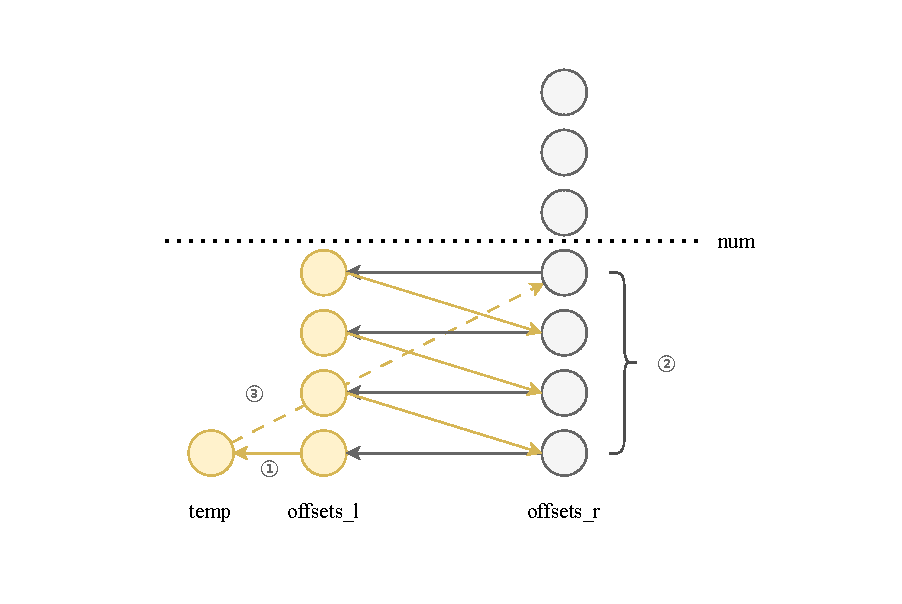
\includegraphics[width=1\textwidth]{cyclicpermu.drawio.pdf}
\end{figure}
\end{center}

\begin{algorithm}[H]
\small
\caption{Cyclic Permutation}\label{CyclicPermutation}
\begin{algorithmic}
    \State temp $\gets A\bigl[\ell +
    \mathrm{offsets}_L[\mathrm{start}_L]\bigr]$ \Comment{(1) preserve the last element in temp variable} 
    
    \State $A\bigl[\ell +
    \mathrm{offsets}_L[\mathrm{start}_L]\bigr] \gets
    A\bigl[r- \mathrm{offsets}_R[\mathrm{start}_R]\bigr]$\Comment{(2) start with the first one}
    
    \For{$j = 1,\dots, \mathrm{num} - 1$}\Comment{main cyclic for loop}

    \State $A\bigl[r - \mathrm{offsets}_R[\mathrm{start}_R + j - 1]\bigr] \gets
    A\bigl[\ell + \mathrm{offsets}_L[\mathrm{start}_L + j]\bigr]$     
    \State $A\bigl[\ell + \mathrm{offsets}_L[\mathrm{start}_L + j]\bigr]
    \gets A\bigl[r - \mathrm{offsets}_R[\mathrm{start}_R + j ]\bigr]$ 

    \EndFor
    \State $A\bigl[r - \mathrm{offsets}_R[\mathrm{start}_R + \mathrm{num} - 1]\bigr] \gets$
    temp \Comment{(3) put the preserved element back to the last place}
\end{algorithmic}
\end{algorithm}

Here we mapped the pseudocode in parts to the steps in the figure, the first step is to preserve the last element in the left buffer block in a temporary variable,
then we doing the cyclic permutation in the main loop, shifting misplaced elements from buffers on one side to the other to make sure they are well partitioned, and finally we put the preserved element back to the last place in the right buffer block.
This rotate-n like method is basically made up of multiple copys from pointers in order to reduce the number of swaps to the minimum, as swaps will constantly overwrite the value in the temporary variable. It is a great improvement over the original Hoare's partition.

We also have adaptions of the Block Lomuto's partition method. Comprehension won't be hard on basis of our fundamental understandings of the classical Lomuto's partition method.

\begin{algorithm}[t!]
    \small
    \caption{One-Pivot Block Partition Lomuto}\samepage\label{algo:single:pivot:partitioning}
    \textbf{procedure} \lomutoone($\textit{A}[1..\textit{n}]$)
    \begin{algorithmic}[1]
        \Require $\textit{n} > 1, \text{Pivot in $\textit{A}[\textit{n}]$}$
        \State $\texttt{p} \gets \textit{A}[\textit{n}]$; 
    \State \textbf{integer} $\text{block}[0, \ldots, \textit{B} - 1]$, $\texttt{i}, \texttt{j} \gets 1$, $\texttt{num} \gets 0$
    \While{$\texttt{j} < \textit{n}$}
    \State $\texttt{t} \gets \text{min}(\textit{B}, \textit{n} - \texttt{j} )$;
\For{$\texttt{c} \gets 0; \texttt{c} < \texttt{t}; \texttt{c} \gets \texttt{c} + 1$} 
                \State $\text{block}[\texttt{num}] \gets \texttt{c}$;
            \State $\texttt{num} \gets \texttt{num} +  (\texttt{p} > \textit{A}[\texttt{j} + \texttt{c}])$;
            \EndFor
            \For{$\texttt{c} \gets 0; \texttt{c} < \texttt{num}; \texttt{c} \gets \texttt{c} + 1$} 
        \State \text{Swap $\textit{A}[\texttt{i}]$ and $\textit{A}[\texttt{j} + \text{block}[\texttt{c}]]$}
        \State $\texttt{i} \gets \texttt{i} + 1$
            \EndFor
            \State $\texttt{num} \gets 0$;
        \State $\texttt{j} \gets \texttt{j} + \texttt{t}$;
        \EndWhile
        \State Swap $\textit{A}[\texttt{i}]$ and $\textit{A}[\textit{n}]$;\\
    \Return $\texttt{i}$;
    \end{algorithmic}
\end{algorithm}
\begin{figure}[t!]
\vspace*{-1.5em}
\centering
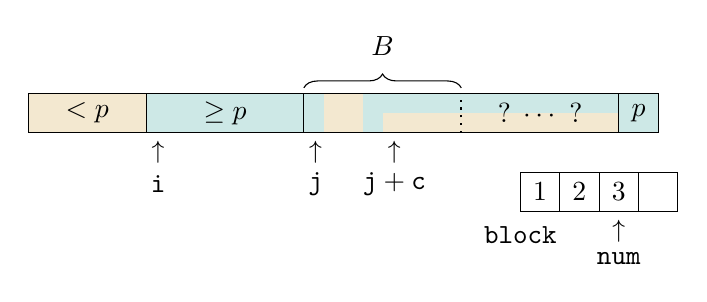
\begin{tikzpicture}[xscale = 1.0]
% main array
\draw[fill=hellgruen!30] (0,0) rectangle (1.5, 0.5);
\draw[fill=dunkelgruen!30] (1.5,0) rectangle (3.5, 0.5);
\draw[fill=dunkelgruen!30] (7.5,0) rectangle (8, 0.5);
\fill[fill=dunkelgruen!30] (4.5,0.25) rectangle (7.5, 0.5);
\fill[fill=hellgruen!30] (4.5,0) rectangle (7.5, 0.25);
\fill[fill=dunkelgruen!30] (3.5,0) rectangle (3.75, 0.5);
\fill[fill=hellgruen!30] (3.75,0) rectangle (4.0, 0.5);
\fill[fill=hellgruen!30] (4,0) rectangle (4.25, 0.5);
\fill[fill=dunkelgruen!30] (4.25,0) rectangle (4.5, 0.5);
\draw (0,0) rectangle (8, 0.5);
\draw (7.5, 0) -- (7.5, 0.5);
\draw (1.5, 0) -- (1.5, 0.5);
\draw (3.5, 0) -- (3.5, 0.5);
\draw[dotted, thick] (5.5, 0) -- (5.5, 0.5);
\node at (7.75, 0.25) {$p$};
\node at (0.75, 0.25) {$< p$};
\node at (2.5, 0.25) {$\geq p$};
\node at (6.5, 0.25) {? $\cdots$ ?};
\node at (1.65, -0.25) {\small$\uparrow$};
\node at (1.65, -0.65) {$\texttt{i}$};
\node at (3.65, -0.25) {\small$\uparrow$};
\node at (3.65, -0.65) {$\texttt{j}$};
\node at (4.65, -0.25) {\small$\uparrow$};
\node at (4.65, -0.65) {$\texttt{j} + \texttt{c}$};
\draw [decorate, decoration={brace,amplitude=5pt},yshift=2pt](3.5,0.5)--(5.5,0.5) node [midway,yshift=15pt]{$B$};
%\draw [step = .25, blue, opacity=0.3] (0, -1.5) grid (\columnwidth, 0.5);
%block
\draw (6.25,-1) rectangle (8.25, -0.5);
\draw (6.25, -1) -- (6.25, -0.5);
\draw (6.75, -1) -- (6.75, -0.5);
\draw (7.25, -1) -- (7.25, -0.5);
\draw (7.75, -1) -- (7.75, -0.5);
\draw (8.25, -1) -- (8.25, -0.5);
\node at (6.5, -0.75) {1};
\node at (7, -0.75) {2};
\node at (7.5, -0.75) {3};
\node at (7.5, -1.25) {\small$\uparrow$};
\node at (7.5, -1.6) {$\texttt{num}$};
\node at (6.25, -1.3) {$\texttt{block}$};

\end{tikzpicture}
\vspace{-1.5em}
%\includegraphics[width=\columnwidth]{fig-lomuto-block.png}
\caption{BlockQuicksort with Lomuto's partitioning scheme.} %Picture depicts the situation where Algorithm~\ref{algo:single:pivot:partitioning} is currently on Line~7 with $\texttt{c} = 4$. So far, the block contains the indexes 1 and 2, representing that $A[\texttt{j} + 1]$ and $A[\texttt{j} + 2]$ are smaller than $p$. In general, given that $\texttt{c}$ has value $c$ and $\texttt{num}$ is \textit{num}, $\texttt{block}[0..\textit{num} - 1]$ contains the indexes (relative to $\texttt{j}$) of all misplaced elements in $A[\texttt{j}..\texttt{j} + c]$. Unlabeled elements have only half the width of the array cell depicting $p$ in the picture.}
\label{fig:lomuto:block:invariant}
\end{figure}

Partition left to the index j is the sub-result of last iteration, we are currently scanning on the block which covers the range of $A[j..j+B-1]$, and the block buffer is used to store the index offsets of the misplaced elements inside.
The first element with index 0 is neglected for being blue -- greater than the pivot, and the yellow elements with index 1 and 2 -- less than the pivot, are stored in the buffer. The third blue element with index 2, temporarily stored in the buffer, will be replaced soon by the next misplaced item in the next iteration that deals with unknown values that can be either less or greater than the pivot.

\begin{algorithm}[t!]
    \small
    \caption{Two-Pivot Block Partition Lomuto}\samepage\label{algo:dual:pivot:partitioning}
    \textbf{procedure} \lomutotwo($\textit{A}[1..\textit{n}]$)
    \begin{algorithmic}[1]
        \Require $n > 1$, \text{Pivots in $\textit{A}[1] \leq \textit{A}[\textit{n}]$}
        \State $\texttt{p} \gets \textit{A}[1]$; $\texttt{q} \gets \textit{A}[n]$; 
    \State \textbf{integer} $\text{block}[0, \ldots, \textit{B} - 1]$
    \State  $\texttt{i}, \texttt{j}, \texttt{k} \gets 2$, $\texttt{num}_{< \texttt{p}}, \texttt{num}_{\leq \texttt{q}} \gets 0$
    \While{$\texttt{k} < \textit{n}$}
    \State $\texttt{t} \gets \text{min}(\textit{B}, \textit{n} - \texttt{k} )$;
\For{$\texttt{c} \gets 0; \texttt{c} < \texttt{t}; \texttt{c} \gets \texttt{c} + 1$} 
            \State $\text{block}[\texttt{num}_{\leq \texttt{q}}] \gets \texttt{c}$;
        \State $\texttt{num}_{\leq \texttt{q}} \gets \texttt{num}_{\leq \texttt{q}} +  (\texttt{q} \geq \textit{A}[\texttt{k} + \texttt{c}])$;
            \EndFor
            \For{$\texttt{c} \gets 0; \texttt{c} < \texttt{num}_{\leq \texttt{q}}; \texttt{c} \gets \texttt{c} + 1$} 
        \State \text{Swap $\textit{A}[\texttt{j} + \texttt{c}]$ and $\textit{A}[\texttt{k} + \text{block}[\texttt{c}]]$}
            \EndFor
            \State $\texttt{k} \gets \texttt{k} + \texttt{t}$;
            \For{$\texttt{c} \gets 0; \texttt{c} < \texttt{num}_{\leq \texttt{q}}; \texttt{c} \gets \texttt{c} + 1$} 
        \State $\text{block}[\texttt{num}_{< \texttt{p}}] \gets \texttt{c}$;
    \State $\texttt{num}_{< \texttt{p}} \gets \texttt{num}_{< \texttt{p}} +  (\texttt{p} > \textit{A}[\texttt{j} + \texttt{c}])$;
            \EndFor
            \For{$\texttt{c} \gets 0; \texttt{c} < \texttt{num}_{< \texttt{p}}; \texttt{c} \gets \texttt{c} + 1$} 
        \State \text{Swap $\textit{A}[\texttt{i}]$ and $\textit{A}[\texttt{j} + \text{block}[\texttt{c}]]$}
        \State $\texttt{i} \gets \texttt{i} + 1$
            \EndFor
            \State $\texttt{j} \gets \texttt{j} + \texttt{num}_{\leq \texttt{q}}$;
    \State $\texttt{num}_{< \texttt{p}}, \texttt{num}_{\leq \texttt{q}} \gets 0$;
        \EndWhile
        \State Swap $\textit{A}[\texttt{i} - 1]$ and $\textit{A}[1]$;
    \State Swap $\textit{A}[\texttt{j}]$ and $\textit{A}[\textit{n}]$;\\
\Return $(\texttt{i} - 1,\texttt{j})$;
    \end{algorithmic}
\end{algorithm}

\begin{figure}[H]
\vspace*{-1em}
\centering
\scalebox{.92}{
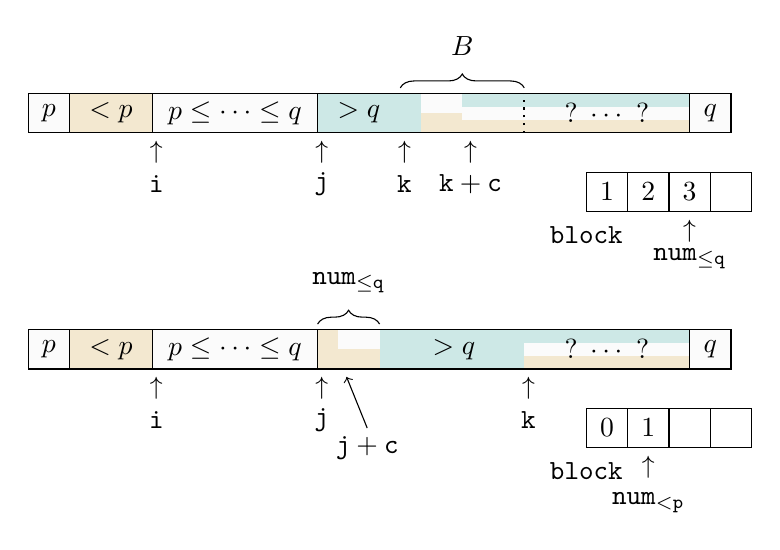
\begin{tikzpicture}[xscale = 1.05, xshift=0.5cm]
\draw[fill=gruen!30] (-0.5, 0) rectangle (0, 0.5);
\draw[fill=hellgruen!30] (0,0) rectangle (1, 0.5);
\draw[fill=gruen!30] (1,0) rectangle (3, 0.5);
\draw[fill=dunkelgruen!30] (3, 0) rectangle (4, 0.5);
\draw[fill=gruen!30] (7.5,0) rectangle (8, 0.5);
\fill[fill=dunkelgruen!30] (4,0) rectangle (4.25, 0.5);
\fill[fill=gruen!30] (4.25,0.25) rectangle (4.75, 0.5);
\fill[fill=hellgruen!30] (4.25,0) rectangle (4.75, 0.25);
\fill[fill=hellgruen!30] (4.75,0) rectangle (7.5, 0.16);
\fill[fill=gruen!30] (4.75,0.16) rectangle (7.5, 0.33);
\fill[fill=dunkelgruen!30] (4.75,0.33) rectangle (7.5, 0.5);


% \fill[fill=hellgruen!30] (4.5,0.25) rectangle (7.5, 0.5);
% \fill[fill=dunkelgruen!30] (3.5,0) rectangle (3.75, 0.5);
% \fill[fill=hellgruen!30] (3.75,0) rectangle (4.0, 0.5);
% \fill[fill=hellgruen!30] (4,0) rectangle (4.25, 0.5);
% \fill[fill=dunkelgruen!30] (4.25,0) rectangle (4.5, 0.5);
\draw (0,0) rectangle (8, 0.5);
\draw (7.5, 0) -- (7.5, 0.5);
%\draw (1, 0) -- (1, 0.5);
%\draw (3.5, 0) -- (3.5, 0.5);
\draw[dotted, thick] (5.5, 0) -- (5.5, 0.5);
\node at (-0.25, 0.25) {$p$};
\node at (7.75, 0.25) {$q$};
\node at (0.5, 0.25) {$< p$};
\node at (2, 0.25) {$p \leq \dots \leq q$};
\node at (3.5, 0.25) {$> q$};
\node at (6.5, 0.25) {? $\cdots$ ?};
\node at (1.05, -0.25) {\small$\uparrow$};
\node at (1.05, -0.65) {$\texttt{i}$};
\node at (3.05, -0.25) {\small$\uparrow$};
\node at (3.05, -0.65) {$\texttt{j}$};
\node at (4.05, -0.25) {\small$\uparrow$};
\node at (4.05, -0.65) {$\texttt{k}$};
\node at (4.85, -0.25) {\small$\uparrow$};
\node at (4.85, -0.65) {$\texttt{k} + \texttt{c}$};
\draw [decorate, decoration={brace,amplitude=5pt},yshift=2pt](4,0.5)--(5.5,0.5) node [midway,yshift=15pt]{$B$};
%\draw [step = .25, blue, opacity=0.3] (0, -1.5) grid (\columnwidth, 0.5);
%block
\draw (6.25,-1) rectangle (8.25, -0.5);
\draw (6.25, -1) -- (6.25, -0.5);
\draw (6.75, -1) -- (6.75, -0.5);
\draw (7.25, -1) -- (7.25, -0.5);
\draw (7.75, -1) -- (7.75, -0.5);
\draw (8.25, -1) -- (8.25, -0.5);
\node at (6.5, -0.75) {1};
\node at (7, -0.75) {2};
\node at (7.5, -0.75) {3};
\node at (7.5, -1.25) {\small$\uparrow$};
\node at (7.5, -1.6) {$\texttt{num}_{\leq \texttt{q}}$};
\node at (6.25, -1.3) {$\texttt{block}$};


\begin{scope}[yshift = -3cm]


% main array
\draw[fill=gruen!30] (-0.5, 0) rectangle (0, 0.5);
\draw[fill=hellgruen!30] (0,0) rectangle (1, 0.5);
\draw[fill=gruen!30] (1,0) rectangle (3, 0.5);
\draw[fill=dunkelgruen!30] (3.75, 0) rectangle (5.5, 0.5);
\draw[fill=gruen!30] (7.5,0) rectangle (8, 0.5);
%\fill[fill=dunkelgruen!30] (4,0) rectangle (4.25, 0.5);
%\fill[fill=gruen!30] (4.25,0.25) rectangle (4.75, 0.5);
%\fill[fill=hellgruen!30] (4.25,0) rectangle (4.75, 0.25);
\fill[fill=hellgruen!30] (5.5,0) rectangle (7.5, 0.16);
\fill[fill=gruen!30] (5.5,0.16) rectangle (7.5, 0.33);
\fill[fill=dunkelgruen!30] (5.5,0.33) rectangle (7.5, 0.5);
\fill[fill=hellgruen!30] (3, 0) rectangle (3.25, 0.5);
\fill[fill=hellgruen!30] (3.25,0.0) rectangle (3.75, 0.25);
\fill[fill=gruen!30] (3.25,0.25) rectangle (3.75, 0.5);


% \fill[fill=hellgruen!30] (4.5,0.25) rectangle (7.5, 0.5);
% \fill[fill=dunkelgruen!30] (3.5,0) rectangle (3.75, 0.5);
% \fill[fill=hellgruen!30] (3.75,0) rectangle (4.0, 0.5);
% \fill[fill=hellgruen!30] (4,0) rectangle (4.25, 0.5);
% \fill[fill=dunkelgruen!30] (4.25,0) rectangle (4.5, 0.5);
\draw (0,0) rectangle (8, 0.5);
\draw (7.5, 0) -- (7.5, 0.5);
%\draw (1, 0) -- (1, 0.5);
%\draw (3.5, 0) -- (3.5, 0.5);
%\draw[dotted, thick] (5.5, 0) -- (5.5, 0.5);
\node at (-0.25, 0.25) {$p$};
\node at (7.75, 0.25) {$q$};
\node at (0.5, 0.25) {$< p$};
\node at (2, 0.25) {$p \leq \dots \leq q$};
\node at (4.65, 0.25) {$> q$};
\node at (6.5, 0.25) {? $\cdots$ ?};
\node at (1.05, -0.25) {\small$\uparrow$};
\node at (1.05, -0.65) {$\texttt{i}$};
\node at (3.05, -0.25) {\small$\uparrow$};
\node at (3.05, -0.65) {$\texttt{j}$};
\node at (5.55, -0.25) {\small$\uparrow$};
\node at (5.55, -0.65) {$\texttt{k}$};
\draw[->] (3.6, -0.75) -- (3.35, - 0.1);
\node at (3.6, -1) {$\texttt{j} + \texttt{c}$};
\draw [decorate, decoration={brace,amplitude=5pt},yshift=2pt](3,0.5)--(3.75,0.5) node [midway,yshift=15pt]{$\texttt{num}_{\leq \texttt{q}}$};
%\draw [step = .25, blue, opacity=0.3] (0, -1.5) grid (\columnwidth, 0.5);
%block
\draw (6.25,-1) rectangle (8.25, -0.5);
\draw (6.25, -1) -- (6.25, -0.5);
\draw (6.75, -1) -- (6.75, -0.5);
\draw (7.25, -1) -- (7.25, -0.5);
\draw (7.75, -1) -- (7.75, -0.5);
\draw (8.25, -1) -- (8.25, -0.5);
\node at (6.5, -0.75) {0};
\node at (7, -0.75) {1};
\node at (7.0, -1.25) {\small$\uparrow$};
\node at (7.0, -1.7) {$\texttt{num}_{< \texttt{p}}$};
\node at (6.25, -1.3) {$\texttt{block}$};
\end{scope}
\end{tikzpicture}}
%\includegraphics[width=\columnwidth]{fig-lomuto-block-2.png}
\vspace*{-2em}
\caption{Lomuto block partitioning with two pivots. Top: Algorithm~\ref{algo:dual:pivot:partitioning}
compares elements with $q$ and is on Line~8 with $\texttt{c} = 3$, cf.~Figure~\ref{fig:lomuto:block:invariant}. Bottom: Algorithm compares the $\texttt{num}_{\leq \texttt{q}}$ elements at most as large as $q$ to $p$. Algorithm is on Line~14 with $\texttt{c} = 1$.}
\label{fig:lomuto:two:block:invariant}
\end{figure}

We can observe that there exists one more pass for 2-Pivot Block Lomuto's partition method than the 1-Pivot one. The first pass compares with the larger pivot $q$ and the second pass compares with the smaller pivot $p$.
The intermediate state between the 2 passes shows a mixture of elements that are less than $p$ and at most as large as $q$ swapped to the exchange area in the first pass. The second pass will then move the elements that are less than $p$ to the left side of the array.

\subsection{rotate-n operations}
\hypertarget{rotate-n}
The rotate-n operation is a common operation in the Quicksort algorithm, where we shift the elements by their indices in batch to get rid of the duplicated swaps, and to make the partitioning process more plain and simple to understand.
This improves slightly the performance of the Quicksort algorithm, and is widely used in tweaked Multi-Pivot QuickSort. The rotate-n operation is defined as follows:
\begin{verbatim}
    rotaten(A, [index1, index2, ... indexn]);
\end{verbatim}
which is equivalent to the following code:
\begin{verbatim}
    T temp = A[index1];
    A[index1] = A[index2];
    ...
    A[indexn] = temp;
\end{verbatim}
In Rust I implemented the rotate-n operation as follows:
\begin{verbatim}
#[inline(always)]
pub unsafe fn rotate_$n<T>(arr: *mut T, idx: [usize; $n]) {
    let tmp = std::ptr::read(arr.add(idx[0]));
    for i in 1..$n {
        ptr::copy_nonoverlapping(arr.add(idx[i]), arr.add(idx[i - 1]), 1);
    }
    ptr::copy_nonoverlapping(&tmp, arr.add(idx[$n - 1]), 1);
}
\end{verbatim}

Using direct pointer manipulation, we can avoid the overhead of the Rust borrow checker and array boundary checking to maximize the performance.


\subsection{Multi-Pivot QuickSort}

\begin{algorithm}[H]
    \caption{Dual-Pivot QuickSort}\label{DualPivotQuickSort}
    \begin{algorithmic}[1]
        % \Procedure{DualPivotQuickSort}{$A, l, r$}
        % \If{$l < r$}
        % \State $p1, p2 \gets \textsc{DualPivotPartition}(A, l, r)$
        % \State \textsc{DualPivotQuickSort}(A, l, p1-1)
        % \State \textsc{DualPivotQuickSort}(A, p1+1, p2-1)
        % \State \textsc{DualPivotQuickSort}(A, p2+1, r)
        % \EndIf
        % \EndProcedure

        \Procedure{DualPivotPartition}{$A, l, r$}
        \State $P1, P2 \gets A[l], A[r]$ \Comment{Pivots}
        \If{$P1 > P2$}
        \State \textsc{Swap}($P1, P2$)
        \EndIf

        \State $less \gets l + 1$
        \State $greater \gets r - 1$

        \State $k \gets l$
        \While{$k \leq greater$}
            \If{$A[k] < P1$} \Comment{If the current element is less than P1}
                \State \textsc{Swap}($A[k], A[less]$) \Comment{Shift the element to the leftmost partition}
                \State $less \gets less + 1$
            \ElsIf{$A[k] > P2$} \Comment{If the current element is greater than P2}
                \While{$A[greater] > P2$ \textbf{and} $k < greater$}
                    \State $greater \gets greater - 1$ \Comment{Find the first element less than P2}
                \EndWhile
                \State \textsc{swap}(A[k], A[greater]) \Comment{Swap to the rightmost partition}
                \State $greater \gets greater - 1$
    
                \If{$A[j] < P1$} \Comment{Double check if another swap is needed}
                    \State \textsc{Swap}($A[k], A[less]$) 
                    \State $less \gets less + 1$
                \EndIf
            \EndIf
            \State $k \gets k + 1$ \Comment{Move to the next element}
        \EndWhile
        \State $less \gets less - 1$
        \State $greater \gets greater + 1$
        \State \textsc{Swap}($A[l], A[less]$) \Comment{Put Pivot1 in the middle}
        \State \textsc{Swap}($A[r], A[greater]$) \Comment{Put Pivot2 in the middle}
        \State \textbf{return} $less, greater$
        \EndProcedure
    \end{algorithmic}
\end{algorithm}

With one more pivot added, the two-pivot Quicksort method is introduced by Vladimir Yaroslavskiy in 2009. It uses 2 pivots selected from each end to split the array into 3 parts.
K stands for the current element being scanned, it will be swapped to the left part, which is accumulated by the less pointer, if it is less than the first pivot or do nothing if it is in the middle part.
Otherwise, if it is greater than the second pivot, it will be swapped to the right part, which is accumulated by the greater pointer.
We will double check the current element at index k after the swap to see if it is less than the first pivot, if so, we will swap it to the left part and move the less pointer to the right.
Hereby, we can see that the Dual-Pivot Quicksort is a generalization of the original Quicksort, and the partitioning method is also a generalization of the original Hoare's partition method but with 2 pivots.

What's attracting is that there was once a debate on whether multiple pivots could enhance the performance, as Sedgewick,
who analyzed a dual-pivot approach with an average of $\frac{32}{15}n \ln n + \bigO{n}$ comparisons in 1978, in constrast to the $2n\ln n + \bigO{n}$ of the standard Quick Sort, considered this prototype to be inferior to the classical Quicksort.
However, the Yaroslavskiy's Dual-Pivot Quicksort has proved a success, with the experimental results showing that it has a less amount of $1.9n\ln n + \bigO{n}$ amortized comparisons, but more swaps,
approximately $0.6n\ln n + \bigO{n}$ which is much greater than the $0.33n\ln n + \bigO{n}$ of the original one, is faster than the original Quicksort in most cases.
It is surprising that even with asymptotically only 5\% of less comparisons and nearly 80\% more swaps, the Dual-Pivot Quicksort still outperforms the original Quicksort in practice.
What makes this more mysterious, is the variation of Yaroslavskiy's partition method that always compares to the larger pivot, by Martin Aumüller and Martin Dietzfelbinger 2013 in their thesis of 'Optimal Partitioning for Dual Pivot Quicksort' \cite{OptimalPartitioningForDualPivotQuicksort}.
The method shows no difference in terms of both comparison and swaps with the original Dual-Pivot Quicksort, but it turned out that it is as fast as the Yaroslavskiy's partition, and even faster than another method along with it, named 'Countering Strategy C', who claimed to have the least 
estimations of $1.8n \ln n + \bigO(n)$ comparisons and $1.6n \ln n + \bigO{n}$ swaps. This is a great example of how the real-world performance could be different from the theoretical analysis. In fact, in their following tests, the 'Countering Strategy C' method was proven to be the slowest among all the 3 methods.

It is noteworthy the there still lies a huge gap between the theoretical analysis and the real-world performance. It is time we broaden our horizon and look for more factors that could contribute more to the change of the performance of the Quicksort algorithm.
The cache misses, branch mis-predictions, and the number of instructions are the things we should take into consideration when we are analyzing on mutated versions of the Quicksort algorithm.
Apparently, the number of pivots plays a significant role, and is one of the factors that could potentially bring a significant change. Let's dive deeper to see the world of 3-Pivots Quicksort.

\begin{algorithm}[H]
    \caption{3-Pivot QuickSort}\label{3PivotQuickSort}
    \begin{algorithmic}[1]
        \Procedure{ThreePivotPartition}{$A, l, r$}
        \State $P1, P2, P3 \gets A[l], A[l+1], A[r]$ \Comment{And sort 3 Pivots in ascending order} 

        \State $i, j \gets l + 2$
        \State $k, l \gets r - 1$
        \While{$j \leq k$}
            % // j moves right until arr[j] >= p2
            % while arr[j].cmp(&p2) == Ordering::Less {
            %     // arr[<i] -> elements that are less than p1, arr[i] is not less than p1
            %     if arr[j].cmp(&p1) == Ordering::Less {
            %         arr.swap_unchecked(i, j);
            %         i += 1;
            %     }
            %     j += 1;
            % }
            \While{$A[j] < P2$} \Comment{Put left side elements less than P2 in order}
                \If{$A[j] < P1$}
                    \State \textsc{Swap}($A[i], A[j]$)
                    \State $i \gets i + 1$
                \EndIf
                \State $j \gets j + 1$
            \EndWhile
            % // k moves left until arr[k] <= p2
            % while arr[k].cmp(&p2) == Ordering::Greater {
			% 	// arr[>l] -> elements that are greater than p3, arr[l] is not greater than p3
			% 	if arr[k].cmp(&p3) == Ordering::Greater {
			% 		arr.swap_unchecked(k, l);
			% 		l -= 1;
			% 	}
			% 	k -= 1;
			% }
            \While{$A[k] > P2$} \Comment{Put right side elements greater than P2 in order}
                \If{$A[k] > P3$}
                    \State \textsc{Swap}($A[k], A[l]$)
                    \State $l \gets l - 1$
                \EndIf
                \State $k \gets k - 1$
            \EndWhile
			% // if j is still less than k
			% if j <= k {
			% 	if arr[j].cmp(&p3) == Ordering::Greater {
			% 		if arr[k].cmp(&p1) == Ordering::Less {
			% 			// if arr[j] > p3 and arr[k] < p1, 
			% 			// rotate arr[j] to k and arr[k] to i because arr[<i] < p1
			% 			rotate3(arr, [j, i, k]);
			% 			i += 1;
			% 		} else {
			% 			// if arr[j] > p3 and arr[k] >= p1,
			% 			// simply swap arr[j] and arr[k]
			% 			arr.swap_unchecked(j, k);
			% 		}
			% 		// at this moment arr[k] must be greater than p3
			% 		// swap it with arr[l] to move it to the right
			% 		arr.swap_unchecked(k, l);
			% 		l -= 1;
			% 	} else { 
			% 		// if arr[j] <= p3, we do the same logic as above
			% 		if arr[k].cmp(&p1) == Ordering::Less {
			% 			rotate3(arr, [j, i, k]);
			% 			i += 1;
			% 		} else {
			% 			arr.swap_unchecked(j, k);
			% 		}
			% 		// at this moment arr[j] must be less than or equal p1
			% 		// arr[k] must be less than or equal p3
			% 	}
			% 	j += 1;
			% 	k -= 1;
			% }
            \If{$j \leq k$}
                \If{$A[j] > P3$} \Comment{Deal with 2 branches when A[j] is greater than P3}
                    \If{$A[k] < P1$}
                        \State \textsc{Rotate3}($A, [j, i, k]$)
                        \State $i \gets i + 1$
                    \Else
                        \State \textsc{Swap}($A[j], A[k]$) \Comment{A[j] > P3 and P2 > A[k] $\ge$ P1}
                    \EndIf
                    \State \textsc{Swap}($A[k], A[l]$)
                    \State $l \gets l - 1$
                \Else \Comment{Deal with 2 branches when A[j] is less than or equal to P3}
                    \If{$A[k] < P1$}
                        \State \textsc{Rotate3}($A, [j, i, k]$)
                        \State $i \gets i + 1$
                    \Else
                        \State \textsc{Swap}($A[j], A[k]$)
                    \EndIf
                \EndIf
                \State $j \gets j + 1, k \gets k - 1$
            \EndIf
        \EndWhile
        \State $i \gets i - 1, j \gets j - 1, k \gets k + 1, l \gets l + 1$
        % rotate3(arr, [left + 1, i, j]);
        \State \textsc{Rotate3}($A, [left + 1, i, j]$)
        % arr.swap_unchecked(left, i);
		% arr.swap_unchecked(right, l);
        \State \textsc{Swap}($A[left], A[i]$)
        \State \textsc{Swap}($A[right], A[l]$)
        \State \textbf{return} $i, j, l$
        \EndProcedure
    \end{algorithmic}
\end{algorithm}


The three-pivot Quicksort, introduced by Shrinu Kushagra, uses the similar hoare-like partition method, is a further generalization of the Dual-Pivot Quicksort.
In the original implementation, the 3 pivots are selected from the leftmost, the second element and the rightmost element of the array, and are sorted in ascending order.
The scanning procedure is similar to the Dual-Pivot Quicksort, but with 3 pivots, the array is divided into 4 parts, and is repeated until all elements are set.
The i, j, k, l pointers are used to scan the array and the elements are swapped to the right places according to the comparison results with the 3 pivots,
where i stands for the leftmost part where elements less than Pivot 1 belongs, j stands for the middle-left part, k stands for the middle-right part and l stands for the rightmost part.
Between j and k stands the unknown region where elements are not yet compared with any of the pivots. 
If the elementa at index j is less than Pivot 2, it is whether swapped to the leftmost part if it is less than Pivot 1,
or do nothing otherwise, since the middle-left part is for elements greater than Pivot1 and less than or equal to Pivot 2.
Same logic applies to the rightmost part, where elements are greater than Pivot 2 and less than or equal to Pivot 3.
These two pre-conditions are checked before the main body of the swapping and rotating procedure, which corresponds to the 2 while loops applied at the top of the main scanning loop.
Afterwards, the real swapping and rotating procedure is applied to the elements at index j and k, which are on the left and right boundaries of the unknown region, need to go to the other side of the array and moved to the right places.

We can simplify this part into a 2 if-else nested block, where the outter if-else block is for the case at index j and the inner one is for the case at index k (vice versa, but we will not go into details here).
Both of them have 2 branches, one for the case where the current element belongs to the leftmost or the rightmost part, and the other for the case where it belongs to the middle-left or the middle-right part.
It is not hard to tell there are $2 \times 2 = 4$ branches in total, and the swapping and rotating procedure is applied to each of them. The following \hyperlink{fig:3pivot}{chart} illustrates the 4 branches and their corresponding actions.

The following figure tags elements belonging to the leftmost, the middle-left, the middle-right and the rightmost part with different colors, and the arrows indicate how they get swapped to be in order.

% \listoffigures
\begin{figure}[H]
    \hypertarget{fig:3pivot}{}
    \caption{3-Pivot Quick Sort}
    \centering
    \hspace*{-0.25\textwidth}
    % \vspace*{+0.1\textheight}
    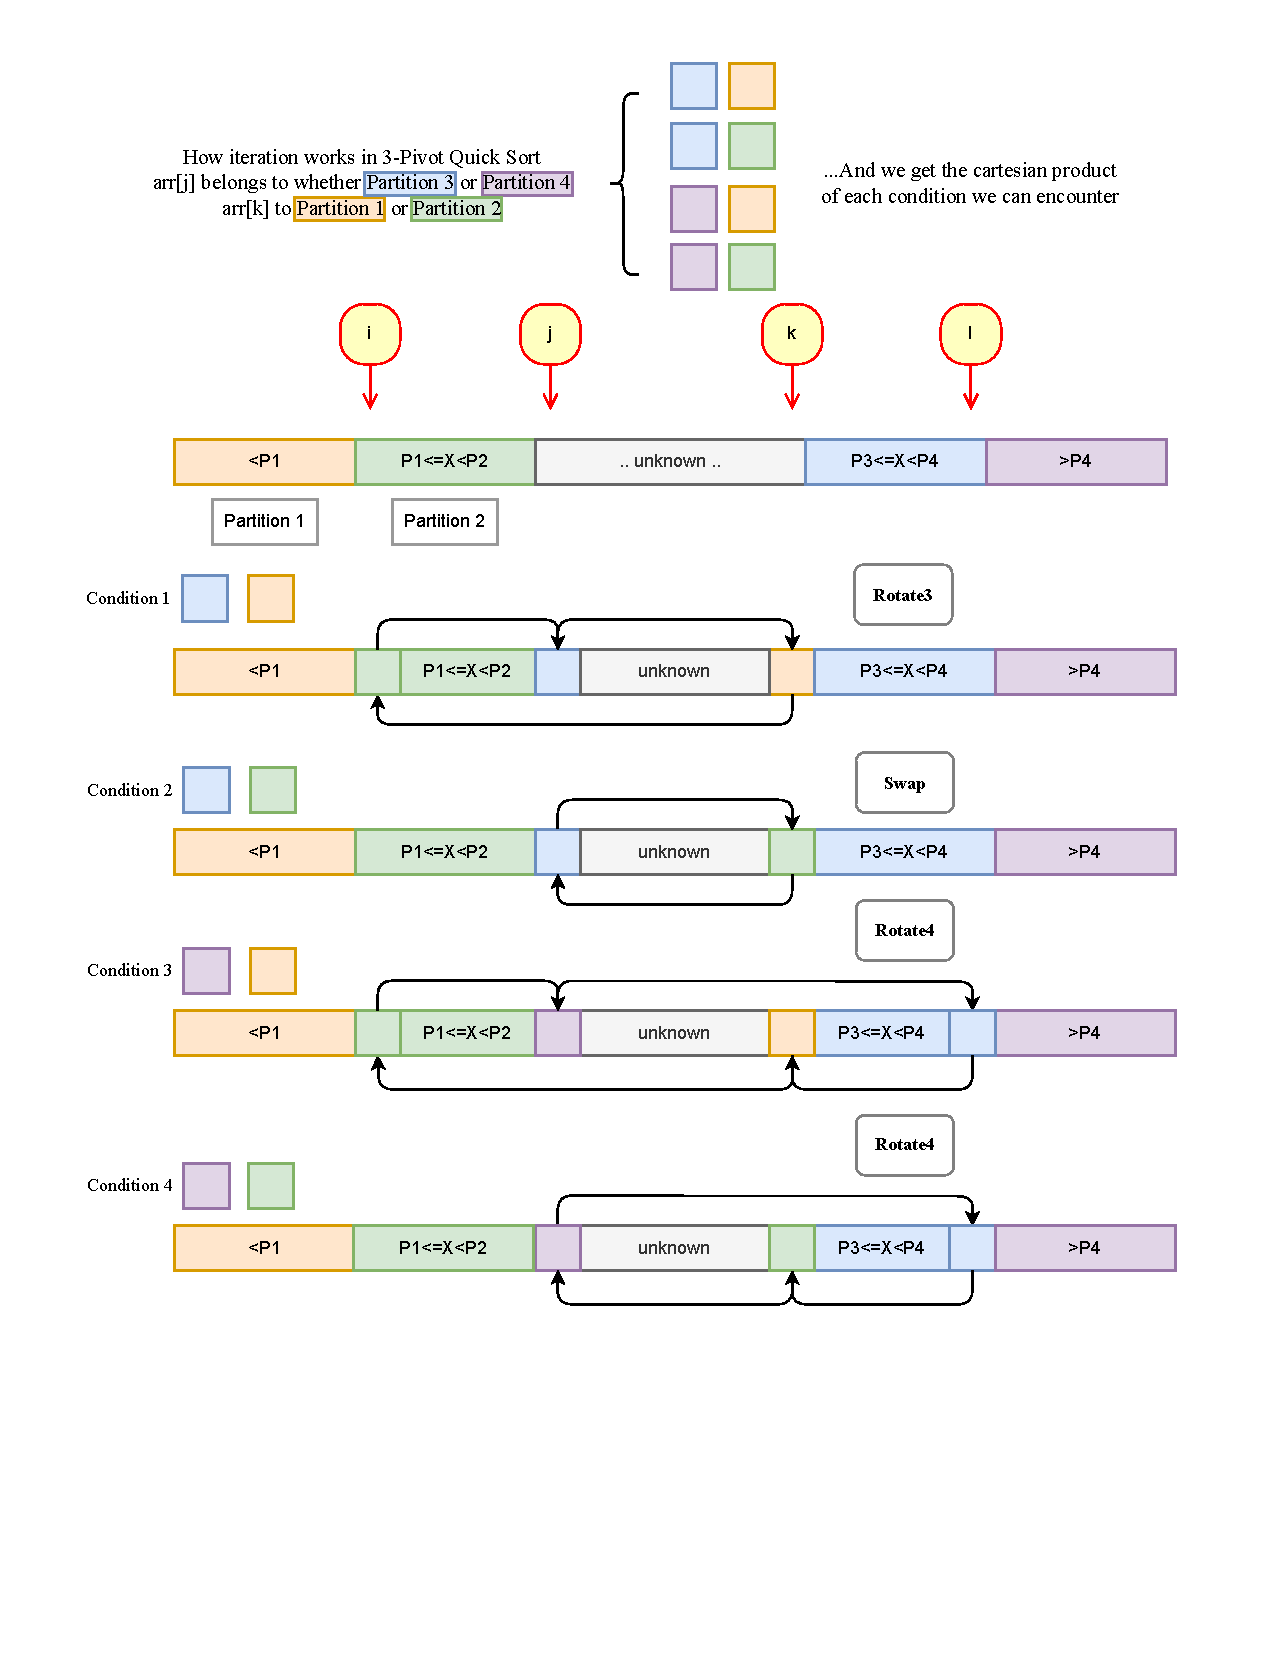
\includegraphics[width=1.5\textwidth]{3pivot.drawio.pdf}
\end{figure}

\section{4-Pivot QuickSort}

\begin{algorithm}[H]
    \small
    \caption{4-Pivot QuickSort}\label{4PivotQuickSort}
    \begin{algorithmic}[1]
        \Procedure{FourPivotPartition}{$A, l, r$}
        
        % let p1: *mut T = &mut arr[left];
		% let p2: *mut T = &mut arr[left + 1];
		% let p3: *mut T = &mut arr[right - 1];
        % let p4: *mut T = &mut arr[right];
        \State $P1, P2, P3, P4 \gets A[l], A[l+1], A[r-1], A[r]$ \Comment{And sort 4 Pivots in order} 

        % let (mut i, mut j, mut k, mut l, mut m) = (left + 2, left + 2, left + 2, right - 2, right - 2);
		% let (p1, p2, p3, p4) = (ptr::read(p1), ptr::read(p2), ptr::read(p3), ptr::read(p4));
        

        % while k <= l {
        %     //        | i              | j              | k
        %     // | < p1 | >= p1 and < p2 | >= p2 and < p3 | unknown
        %     while arr[k].cmp(&p3) == Ordering::Less {
        %         if arr[k].cmp(&p1) == Ordering::Less {
        %             rotate3(arr, [k, j, i]);
        %             i += 1;
        %             j += 1;
        %         } else if arr[k].cmp(&p2) == Ordering::Less {
        %             arr.swap_unchecked(k, j);
        %             j += 1;
        %         }
        %         k += 1;
        %     }
        \State $i, j, k, l, m \gets l + 2, l + 2, l + 2, r - 2, r - 2$
        \While{$k \leq l$}
            \While{$A[k] < P3$} \Comment{Put left side elements less than P3 in order}
                \If{$A[k] < P1$}
                    \State \textsc{Rotate3}($A, [k, j, i]$)
                    \State $i \gets i + 1$, $j \gets j + 1$
                \ElsIf{$A[k] < P2$}
                    \State \textsc{Swap}($A[k], A[j]$)
                    \State $j \gets j + 1$
                \EndIf
                \State $k \gets k + 1$
            \EndWhile
            % //        | l              | m              | 
            % // | >= p3 and < p4 | unknown
            % while arr[l].cmp(&p3) == Ordering::Greater {
            %     if arr[l].cmp(&p4) == Ordering::Greater {
            %         arr.swap_unchecked(l, m);
            %         m -= 1;
            %     }
            %     l -= 1;
            % }
            \While{$A[l] > P3$} \Comment{Put right side elements greater than P3 in order}
                \If{$A[l] > P4$}
                    \State \textsc{Swap}($A[l], A[m]$)
                    \State $m \gets m - 1$
                \EndIf
                \State $l \gets l - 1$
            \EndWhile
        %     if k <= l {
        %         if arr[k].cmp(&p4) == Ordering::Less {
        %             // arr[k] > p3, arr[l] < p3
        %             if arr[l].cmp(&p1) == Ordering::Less {
        %                 rotate4(arr, [k, j, i, l]);
        %                 i += 1;
        %                 j += 1;
        %             } else if arr[l].cmp(&p2) == Ordering::Less {
        %                 rotate3(arr, [k, j, l]);
        %                 j += 1;
        %             } else {
        %                 arr.swap_unchecked(k, l);
        %             }
        \If {$k \leq l$} \Comment{Start manipulation on the boundaries of unknown region}
            \If{$A[k] < P4$} \Comment{Deal with 3 branches when A[k] is less than P4}
                \If{$A[l] < P1$}
                    \State \textsc{Rotate4}($A, [k, j, i, l]$)
                    \State $i \gets i + 1$, $j \gets j + 1$
                \ElsIf{$A[l] < P2$}
                    \State \textsc{Rotate3}($A, [k, j, l]$)
                    \State $j \gets j + 1$
                \Else
                    \State \textsc{Swap}($A[k], A[l]$)
                \EndIf
        %         } else {
        %             // arr[k] > p4, arr[l] < p3
        %             if arr[l].cmp(&p2) == Ordering::Greater { // arr[l] goes to (p2, p3), increase k
        %                 rotate3(arr, [k, l, m]);
        %             } else if arr[l].cmp(&p1) == Ordering::Greater { // arr[l] goes to (p1, p2), increase j and k
        %                 rotate4(arr, [k, j, l, m]);
        %                 j += 1;
        %             } else { // arr[l] goes to leftmost side
        %                 rotate5(arr, [k, j, i, l, m]);
        %                 i += 1;
        %                 j += 1;
        %             }
        %             m -= 1;
        %         }
        %         k += 1;
        %         l -= 1;
        %     }
        % }
            \Else \Comment{Deal with 3 branches when A[k] is greater than P4}
                \If{$A[l] > P2$}
                    \State \textsc{Rotate3}($A, [k, l, m]$)
                \ElsIf{$A[l] > P1$}
                    \State \textsc{Rotate4}($A, [k, j, l, m]$)
                    \State $j \gets j + 1$
                \Else
                    \State \textsc{Rotate5}($A, [k, j, i, l, m]$)
                    \State $i \gets i + 1$, $j \gets j + 1$
                \EndIf
                \State $m \gets m - 1$
            \EndIf
            \State $k \gets k + 1$, $l \gets l - 1$
        \EndIf
        \algstore{4pivots}
    \end{algorithmic}
\end{algorithm}

\begin{algorithm}[H]
    \small
    \caption{4-Pivot QuickSort (Continued)}\label{4PivotQuickSort2}
    \begin{algorithmic}[1]
        \algrestore{4pivots}
        \EndWhile
        % i -= 1;
        % j -= 1;
        % // k -= 1;
        % l += 1;
        % m += 1;
        \State $i \gets i - 1, j \gets j - 1, k \gets k - 1, l \gets l + 1, m \gets m + 1$
        % // i, j, l, m are indexes of pivot 1, 2, 3, 4
        % // Here is the place rotate3 can't be replaced by arr.rotate_left
        % // because the indexes (left + 1 > i ?) are not always ascending
        % // so it could lead to a panic
        % // anyway, I leave the rotate_n macro for you to try out in `src/util.rs`
        % rotate3(arr, [left + 1, i, j]);
        % i -= 1;
        % arr.swap_unchecked(left, i);
        
        % rotate3(arr, [right - 1, m, l]);
        % m += 1;
        % arr.swap_unchecked(right, m);
        \State \textsc{Rotate3}($A, [left + 1, i, j]$)
        \State $i \gets i - 1$
        \State \textsc{Swap}($A[left], A[i]$)
        \State \textsc{Rotate3}($A, [right - 1, m, l]$)
        \State $m \gets m + 1$
        \State \textsc{Swap}($A[right], A[m]$)
        \EndProcedure
    \end{algorithmic}
\end{algorithm}

As long as the number of pivots increases, the number of branches will grow linearly, and the complexity of the partitioning method will also inflate.
Thankfully, for 4-Pivot QuickSort, \hypertarget{2MoreBranches}we are just adding two more branches (As showed in the blue-red and purple-red branches in the \hyperlink{fig:4pivot}{chart} below)
compared with the $2 \times 2 = 4$ branches for 3-Pivots into considerations and the branching logic is still under control.
We declare this as the balanced partition\hypertarget{BalancedPartition} layout that we are using, where each side of the array is filled with $\frac{N + 1}{2}$ partitions for odd number $N$ pivots,
or one side with $\frac{N}{2}$ partitions and $\frac{N}{2} + 1$ on the other. The comparisons take place like looking for a value in a binary search tree (BST), for instance when there are 3 pivots in total, comparing with the Pivot 2 first, then the Pivot 1 or Pivot 3.
This search tree is of depth 2 and if we using a unbalanced BST that puts Pivot 1 or Pivot 3 on top, we would have a tree with depth 3, which is not efficient. Bearing this premise in mind, it is not hard to tell that we are going to have 9 branches for 5-Pivot QuickSort (3 partitions on each side, $3 \times 3 = 9$) and 12 branches for 6-Pivot QuickSort (3 partitions on one side and 4 on the other, $3 \times 4 = 12$).
The complexity of the partitioning method is growing way too far and thus only 4-Pivot QuickSort will be discussed in this thesis. In the \cite{HowGoodIsMultiPivotQuicksort}{'how good is multi-pivot quicksort'} paper, the author sketched an extremal tree for seven pivots in fig 10. It seems to differ from the balanced BST I was expecting and due to the packed time I was given,
this question should be given to the future work to analyze whether it is the optimal scheme for 7-Pivots or not.

% TODO: talk about the similar layout that has been illustrated on page 23 of 'how good is multi-pivot quicksort' paper,
% but it only analyzed the odd number pivots and the even number pivots need to be further discussed.
Right after finishing the 4-Pivots implementation, I surprisingly found that similar layout has been depicted in the subsection 7.4
of the thesis \textit{'How good is Multi-Pivot Quicksort'} \cite{HowGoodIsMultiPivotQuicksort} on page 23, where the odd number of pivots are analyzed.
It uses the same \hyperlink{rotate-n}{rotate-n} operation to rearrange the elements in large sizes, and is a key in the partitioning method that
iteratively shrink the middle unknown region and expand the left and right parts. 
For better understanding, a completed visualization on the iterations will be provided right below with the chart of 4-Pivot QuickSort.

\begin{figure}[H]
    \hypertarget{fig:4pivot}{}
    \caption{4-Pivot Quick Sort}
    \centering
    \hspace*{-0.25\textwidth}
    % \vspace*{+0.1\textheight}
    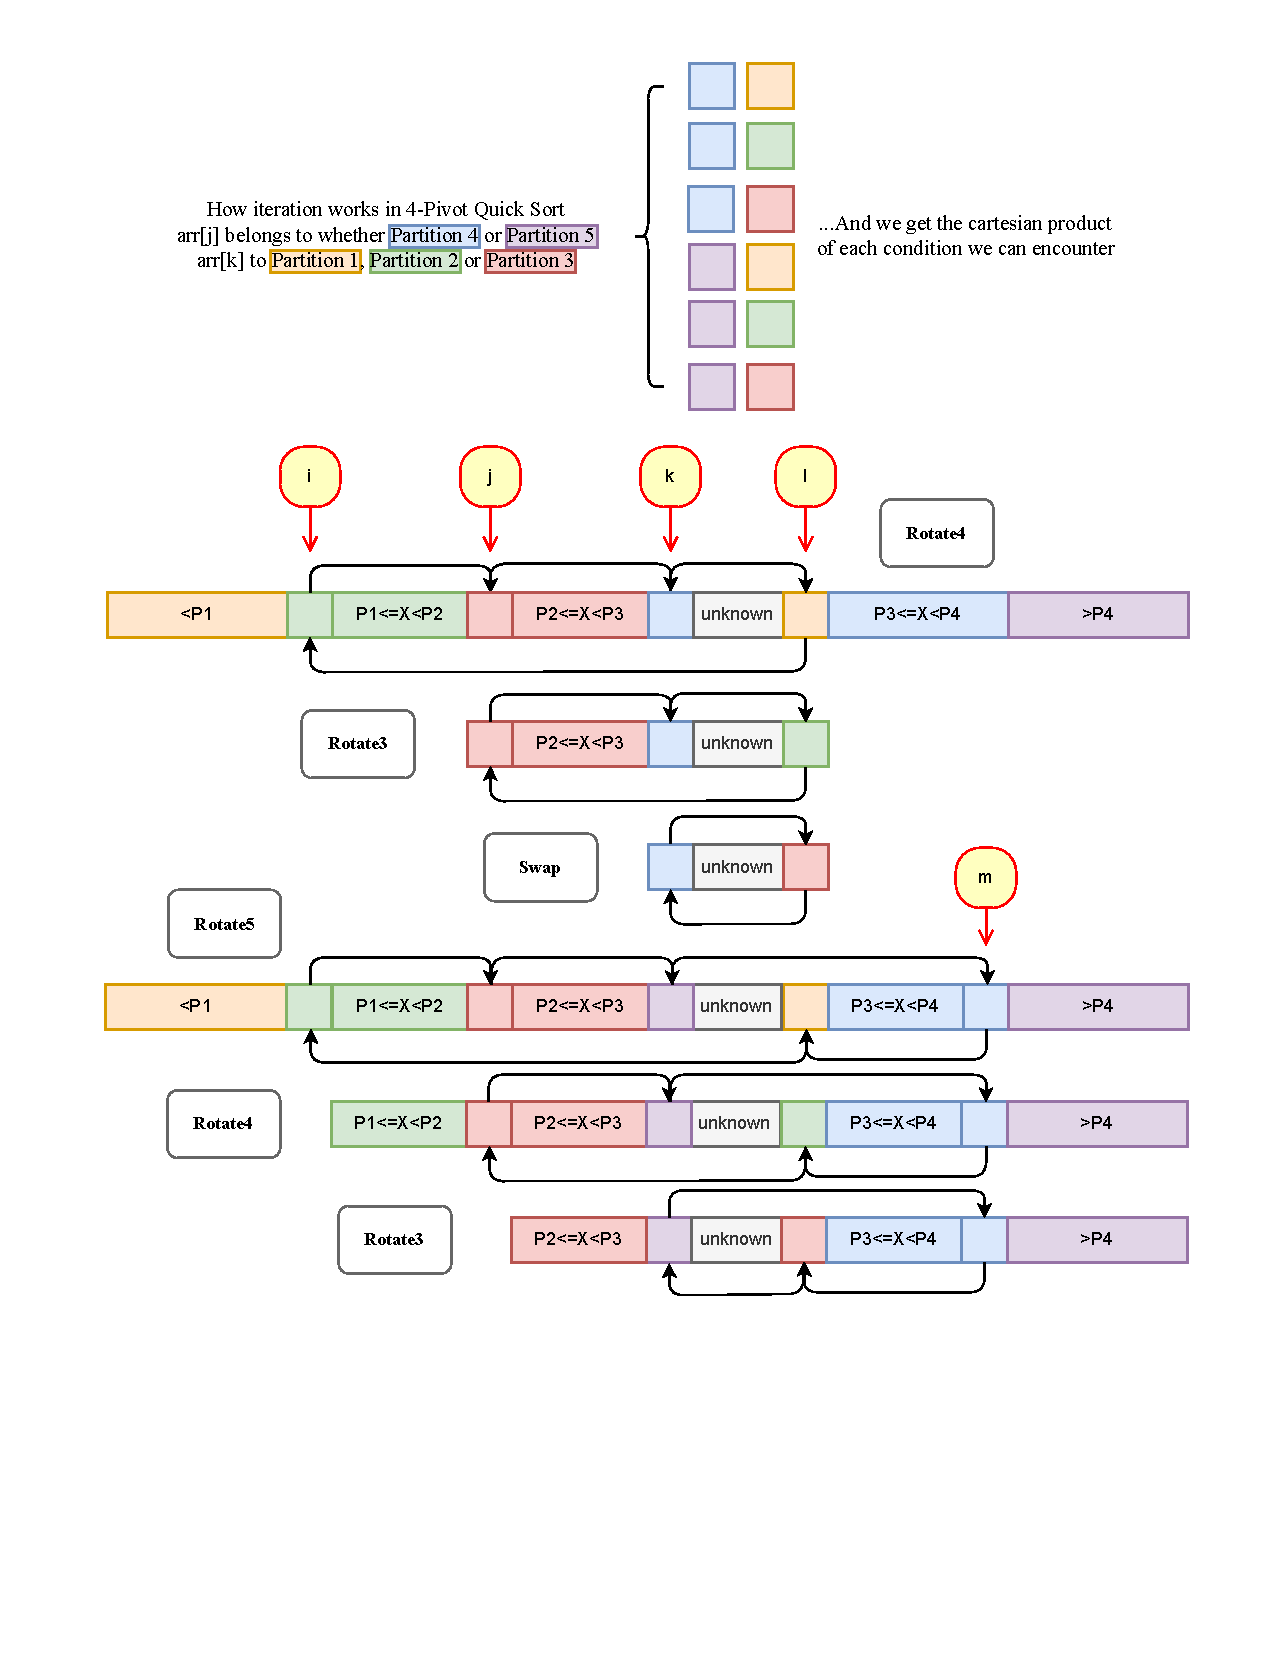
\includegraphics[width=1.5\textwidth]{4pivot.drawio.pdf}
\end{figure}


\section{Analysis}
The analysis on the results of Branch Misses, Cache Misses, Instructions and Time will be conducted below with regard to the Multi-Pivot QuickSorts with traditional partitions.
The details regarding to the testing machine, environment and compiler settings are listed as follows:
\footnote{'opt-level=3' is equivalent to '-O3', 'codegen-units=1' is equivalent to '-fno-merge-all-constants', 'lto="thin"' is equivalent to '-flto=thin' in GCC.} are as follows:
\begin{center}
    \begin{tabular}{ |c|c|c|c|c| }
        \hline
        \multicolumn{2}{ | c | }{CPU}  & \multicolumn{3}{ c | }{Cache} \\
        \hline
        \multicolumn{2}{ | c | }{R7 3700x @4.3GHz Overclocked} & L1 8x32KB & L2 8x512KB & L3 2x16MB \\
        \hline
    \end{tabular}
\end{center}
\begin{center}
    \begin{tabular}{ |c|c|c| }
        \hline
        RAM  & OS           & Compiler \\
        \hline
        16GB & GNU/Linux Ubuntu 22.04 & Rustc 1.78.0 +Nightly \\
        \hline
        \textbf{Rustc Flags} & \multicolumn{2}{ c | }{opt-level=3,codegen-units=1,lto="thin"} \\
        \hline
    \end{tabular}
\end{center}

All the tests presented above are benchmarked using the criterion library, drawing inspiration from the Haskell criterion library, renowned for its strength, robustness and user-friendliness in benchmarking Rust crates.
Tests are organized into groups, with each group a collection of benchmarks that are executed in sequence, comprises of a set of testing functions that are executed under identical environments.
Each test operates within a black box, constraining the compiler from applying overly aggressive optimizations, such as removing instructions it deems rebundant.
The criterion-perf-events plugin is also adapted to capture the hardware events of the CPU as an addition, with the help of the well-established profiling tool $perf$ on Linux. The decision to forego cachegrind in favor of $perf$ was because cachegrind is a simulation tool on the cache misses and introduces a huge overhead on the runtime,
in previous tests with perf, the overall runtime demonstrated runtime deviation of at least 200\% difference with the real-world performance. The use of cachegrind was rejected compared with $perf$.
perf is a more lightweight tool that suits our needs and the results produced are more reliable in respect. Previous tests with cachegrind \hyperlink{cachegrindresult}{`} are given in the appendix for further references.

The compiler flags passed in remain consistent for all the tests, and the tests are conducted on the same machine with the same environment,
with 3 seconds of warm-up time, followed by a 5-seconds duration of measurement for each test. The results are obtained and then calculated over regression tests featuring arrays with $10^2 - 10^7$ elements,
filtering out the outliers. Each sub-test is collected with the mean, standard deviation and median values. The results are shown in the figures below.
The x-axis is uniformed to the size of the array in logarithmic scale, and the y-axis is the average number of events captured by the perf tool or the average running time per element, unit in μs.
Standard deviations will be showed as transparent areas around the polyline of mean values, denoted in colors following their respective lines.
% The next part of the thesis will be the implementation of the Multi-Pivot Quicksort and the BlockQuickSort,
% followed by the analysis of the results and the comparisons on the performance of the above algorithms using traditional partition methods.
\begin{center}
\begin{figure}[H]
    \hypertarget{fig:classicalbranchmiss}{}
    \caption{Classical QuickSort Branch Misses}
    \centering
    \hspace*{-0.27\textwidth}
    % \vspace*{+0.1\textheight}
    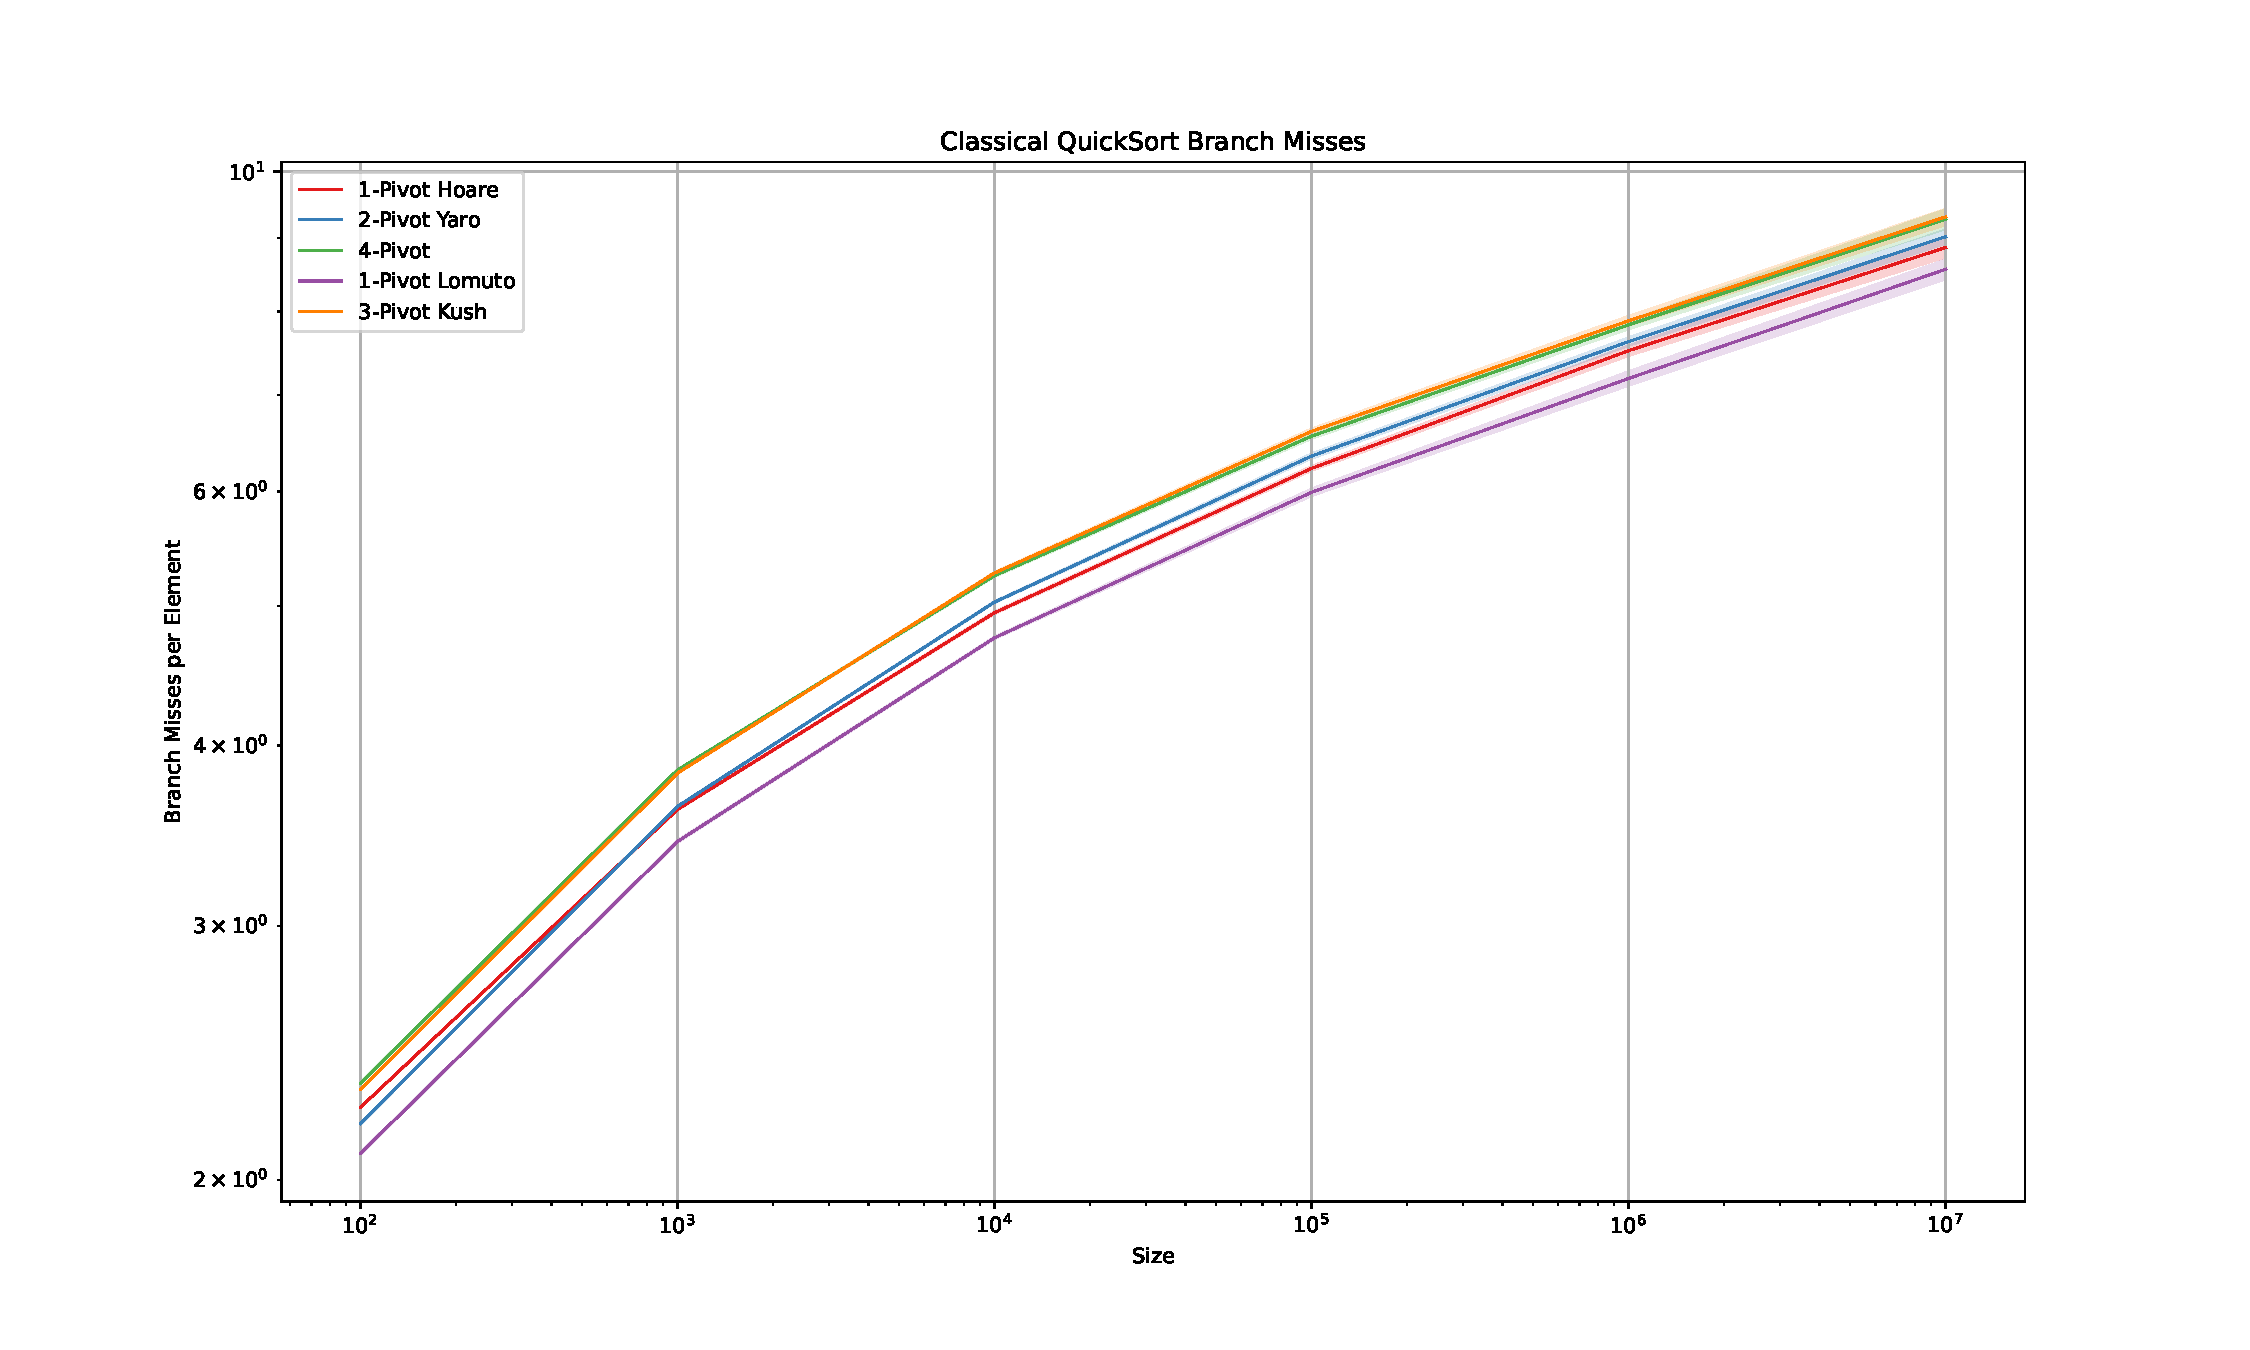
\includegraphics[width=1.5\textwidth]{Classical QuickSort Branch Misses.pdf}
\end{figure}
\end{center}

From the global perspective, after a notable short rocket on branch misses for array sizes below $10^4$, the growth seem to level off for all the partition methods afterwards and go stablized. 
The 4-Pivot partition's branch misses go over the 3-Pivot Kushagra's partition method, and so for the 1-Pivot Hoare partition which has more branch misses over 2-Pivot Yaroslavskiy's method for small arrays.
But soon situations shifted when the size of the array exceeds $10^4$, 4-Pivot and 1-Pivot Hoare emerge better branch behaviors than 3-Pivot and 2-Pivot partition methods.

\begin{center}
    \small
    \begin{tabular}{ |c c | c | }
        \hline
        Branch Misses   & Size     & Mean         \\
        \hline
        1-Pivot Hoare   & 100000   & 622681.46    \\
                        & 1000000  & 7514512.06   \\
                        & 10000000 & 88601386.65  \\
        \hline
        1-Pivot Lomuto  & 100000   & 599369.59    \\
                        & 1000000  & 7188431.33   \\
                        & 10000000 & 85572728.60  \\
        \hline
        2-Pivot Yaro    & 100000   & 635045.30    \\
                        & 1000000  & 7624533.45   \\
                        & 10000000 & 90144952.00  \\
        \hline
        3-Pivot Kush    & 100000   & 660656.78    \\
                        & 1000000  & 7881473.75   \\
                        & 10000000 & 93039500.90  \\
        \hline
        4-Pivot         & 100000   & 655540.97    \\
                        & 1000000  & 7831009.19   \\
                        & 10000000 & 92702517.35  \\
        \hline
    \end{tabular}
    \end{center}

Zooming in, the mean values exhibit minimal variances between the 1-Pivot Hoare and 1-Pivot Lomuto partition methods when the size scales,
it makes sense that the 1-Pivot Hoare's partition method tend to always have a slightly higher mean of branch misses than the 1-Pivot Lomuto's partition method, due to its scheme to locate and swap 2 out-of-order elements, while only 1 for Lomuto's.
We are bound to have some more branch misses in the former case. Meanwhile, 2-Pivot Yaroslavskiy's partition method presents a slightly higher mean of branch misses than both 1-Pivot methods, likely owing to the introduction of additional branches with the second pivot.
Down follows 2-Pivot is the 3-Pivot Kushagra's method, also holds higher mean of branch misses than its fellow methods with less pivots, with more significant differences.

While the complexities scale linearly with the number of pivots, the standard deviation grows rapidly as the size of array exceeds $10^4$, and the standard variation explodes after $10^6$ for all methods, displayed as the transparent areas around lines of mean values.

Things go beyond our expectations, the 4-Pivot partition shows superior statistics of branch misses than the 3-Pivot partition method for larger arrays, which is a surprise to us,
even though it has slightly higher means of branch misses than the 2-Pivot Yaroslavskiy's partition method in general, the standard deviation remains at a high level indicating
the possible instabilities of the 4-Pivot partition method brought by 2 more branches \hypertarget{2MoreBranches}{`} that 1 more pivot introduced. It's intriguing to observe that more pivots could potentially reduce branch misses, challenging conventional assumptions.
It might be that the layout of 'balanced partition' we are using is more friendly to the CPU's branch predictor, but yet to explain why 2 more branches could bring better effects. This warrants further investigation in future works, further expand our understandings on the Multi-Pivot Quicksort algorithm. 

Apart from the branch misses, cache misses also merit attention due to their potential impact, which is what we are going to shift our focus to.

\begin{figure}[H]
    \hypertarget{fig:classicalcachemiss}{}
    \caption{Classical QuickSort Cache Misses}
    \centering
    \hspace*{-0.27\textwidth}
    % \vspace*{+0.1\textheight}
    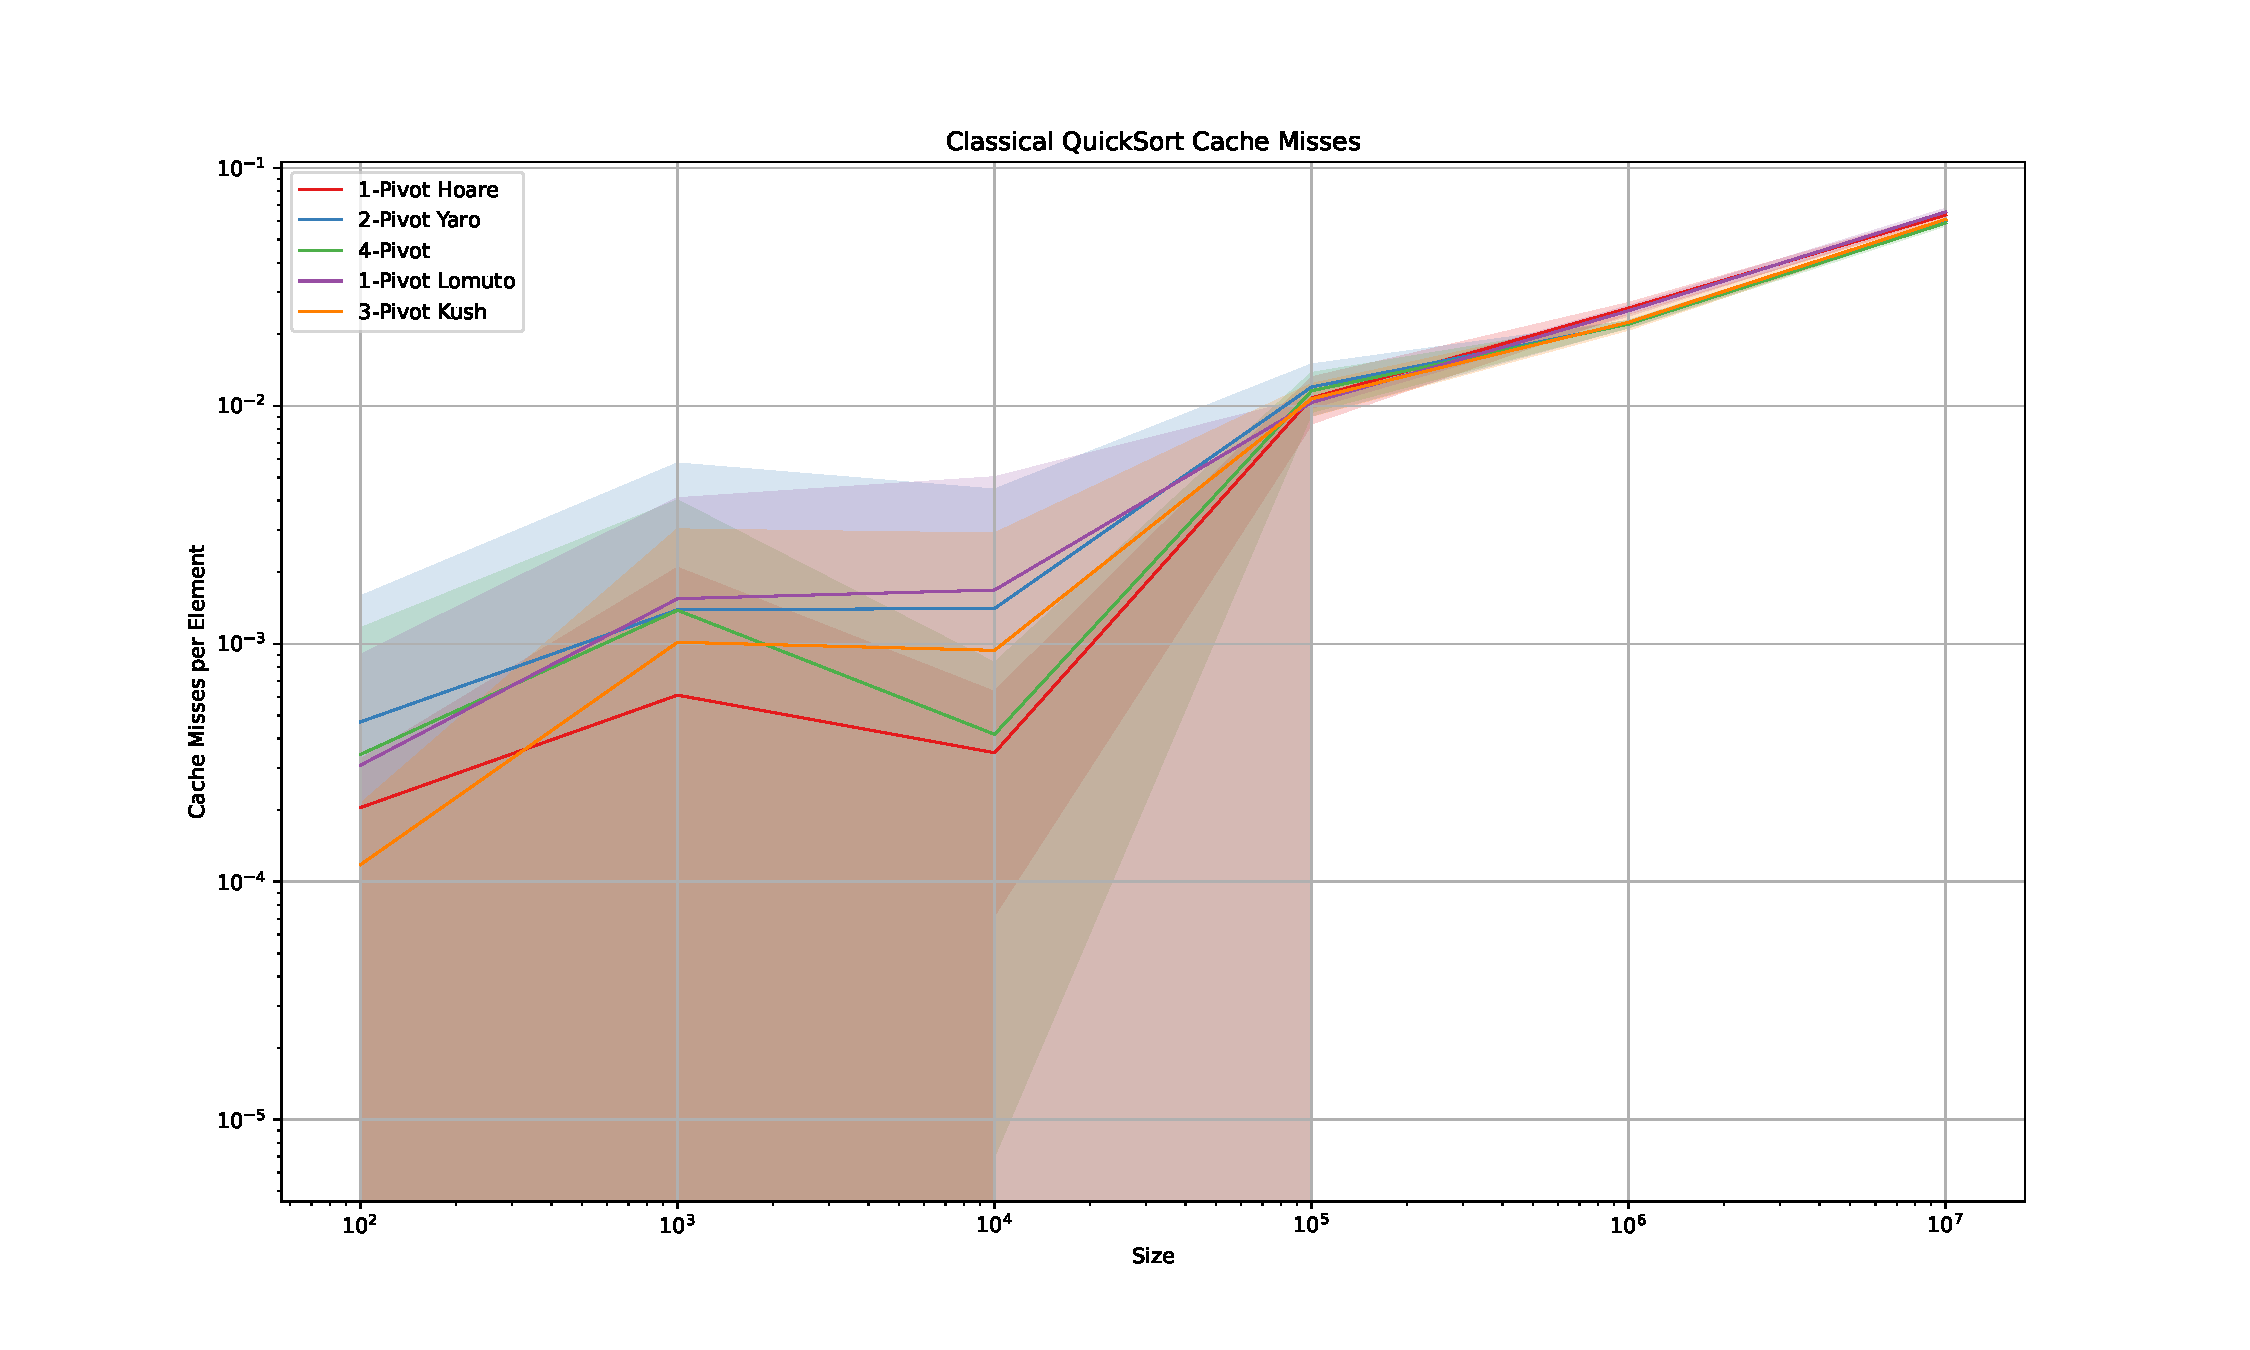
\includegraphics[width=1.5\textwidth]{Classical QuickSort Cache Misses.pdf}
\end{figure}

The macro trend reveals the outburst of cache misses' means when scaling from $10^4$ to $10^5$, possibly indicative of L1 cache saturation.
Prior to this, the cache misses remained relatively low by their means even with the messy and irregular standard deviations still being there.
CPU will run out of L1 cache for size $10^5$ as $10^5 \times 4 {bytes} / element = 4 \times 10^5 {bytes}$, exceeding the total L1 cache capacity for about $8 \times 32Kb = 2.62144 \times 10^5 bytes$ while the spatial locality of the elements might still struggle to mitigate the L2 cache misses at a low level.
Given that L2 misses produce much larger latencies than L1 misses, the performance of the algorithm seriously suffered as it awaits the main memory, thereby amplifies the differences between these algorithms. This disparity stablized and converged after $10^5$, where 2-Pivot Yaroslavskiy, 3-Pivot Kushagra and 4-Pivot partition
exhibit slow and steady increase of cache misses gradually, while 1-Pivot Hoare and Lomuto partition methods still going little bit upwards. However, all the partition methods seem to reach about similar cache misses for $10^7$ elements. This could be due to the magic of modern CPU's cache management, where L3 cache is shared among cores,
in my case among CCDs (Core Complex Die) and the memory controller, so the cache misses are not that sensitive to the size of the array.
Changes in rapid growth of standard deviation is also noteworthy, indicating the dramatic influences caused by the cache misses when the size of the array under $10^4$.

In 1-Pivot tests, Lomuto shows much higher cache misses than Hoare for smaller arrays, likely due to the fact that Lomuto's partition method's tendency for more overlapping swaps than Hoare's,
where most swaps take on the elements that are already in the right place. As the number of pivots grow, the cache misses seem to decrease, particularly evident in the 4-Pivot version,
This lends credence to the claim that choosing more than one pivots can reduce duplicated memory access and cache misses. However, concerns persist regarding the high standard deviation levels.

\begin{center}
\small
\begin{tabular}{ |c c | c | }
    \hline
    Cache Misses    & Size     & Mean           \\
    \hline
    1-Pivot Hoare   & 100000   & 1079.6629      \\
                    & 1000000  & 25764.5000     \\
                    & 10000000 & 634608.9000    \\
    \hline
    1-Pivot Lomuto  & 100000   & 1033.2760      \\
                    & 1000000  & 25119.6125     \\
                    & 10000000 & 653495.7500    \\
    \hline
    2-Pivot Yaro    & 100000   & 1200.8078      \\
                    & 1000000  & 22058.5875     \\
                    & 10000000 & 598454.2000    \\
    \hline
    3-Pivot Kush    & 100000   & 1071.0240      \\
                    & 1000000  & 22472.1100     \\
                    & 10000000 & 608203.3000    \\
    \hline
    4-Pivot         & 100000   & 1158.2534      \\
                    & 1000000  & 22077.3200     \\
                    & 10000000 & 587479.3000    \\
    \hline
\end{tabular}
\end{center}

Among larger array test cases on all variations, the 2-Pivot Yaroslavskiy's partition method consistently hold the most stable combination of both cache misses and branch misses, with stable standard deviations.
Comparatively, 1-Pivot Hoare's and Lomuto's partitions show less branch misses but more cache misses, while the opposite holds true for 3 and 4-Pivot methods. This underscores Yaroslavskiy's scheme as striking a balance between performance and deterministic behavior, aligning with optimistic expectations for algorithm efficiency. 

However for 3-Pivots, the cache behavior observed didn't seem to fully comply with the theoretical analysis that it is cache friendlier than classical and Yaroslavskiy's 2-Pivot QuickSorts, 
the cache misses are higher than the 2-Pivot Yaroslavskiy's partition method when the array size exceeds $10^6$. The correlation between cache misses and the number of pivots remains unclear.
Contrary to the conclusion drawn from experiments carried out by Kushagra's team, which attribute the improvements on Multi-Pivots QuickSort to enhanced cache behaviors
\cite{Kushagra}, the tests conducted show that the cache misses do not consistently decrease with more pivots. For instance, the 3-Pivot Kushagra's method shows more cache misses than the 2-Pivot Yaroslavskiy's,
despite demonstrating better runtime performance. These effects are not yet fully understood and need further discussions and investigations, particularly given the potential optimizations introduced by the Rust compiler,
whose is based on top of LLVM (Native LLVM as the Rust's bootstrapped backend codegen component Cranelift is far from being mature on x86 architecture), that might have optimized the code in a different way that the cache behaviors are not well reflected in the results, although I enabled the most aggressive optimizations flags in the compiler settings
and they are similar as GCC and Clang's. They also reported that their 7-Pivot QuickSort has worse performance than the 3-Pivot QuickSort as a result of poor cache behaviors, which is not yet tested in this thesis.
But with the counter examples we have, we need to be more cautious about leveraging how much propotions of the performance improvements are due to better cache behaviors. It is still a topic for further research.
We will discuss about the complicated relationships further when we finish up the analysis on the instructions and time.

In the parts below, we will continue to seek more exceptions that could shift our opinions on the connections between cache and algorithm efficiency.

\begin{figure}[H]
    \hypertarget{fig:classicalcpucycles}{}
    \caption{Classical QuickSort CPU Cycles}
    \centering
    \hspace*{-0.27\textwidth}
    % \vspace*{+0.1\textheight}
    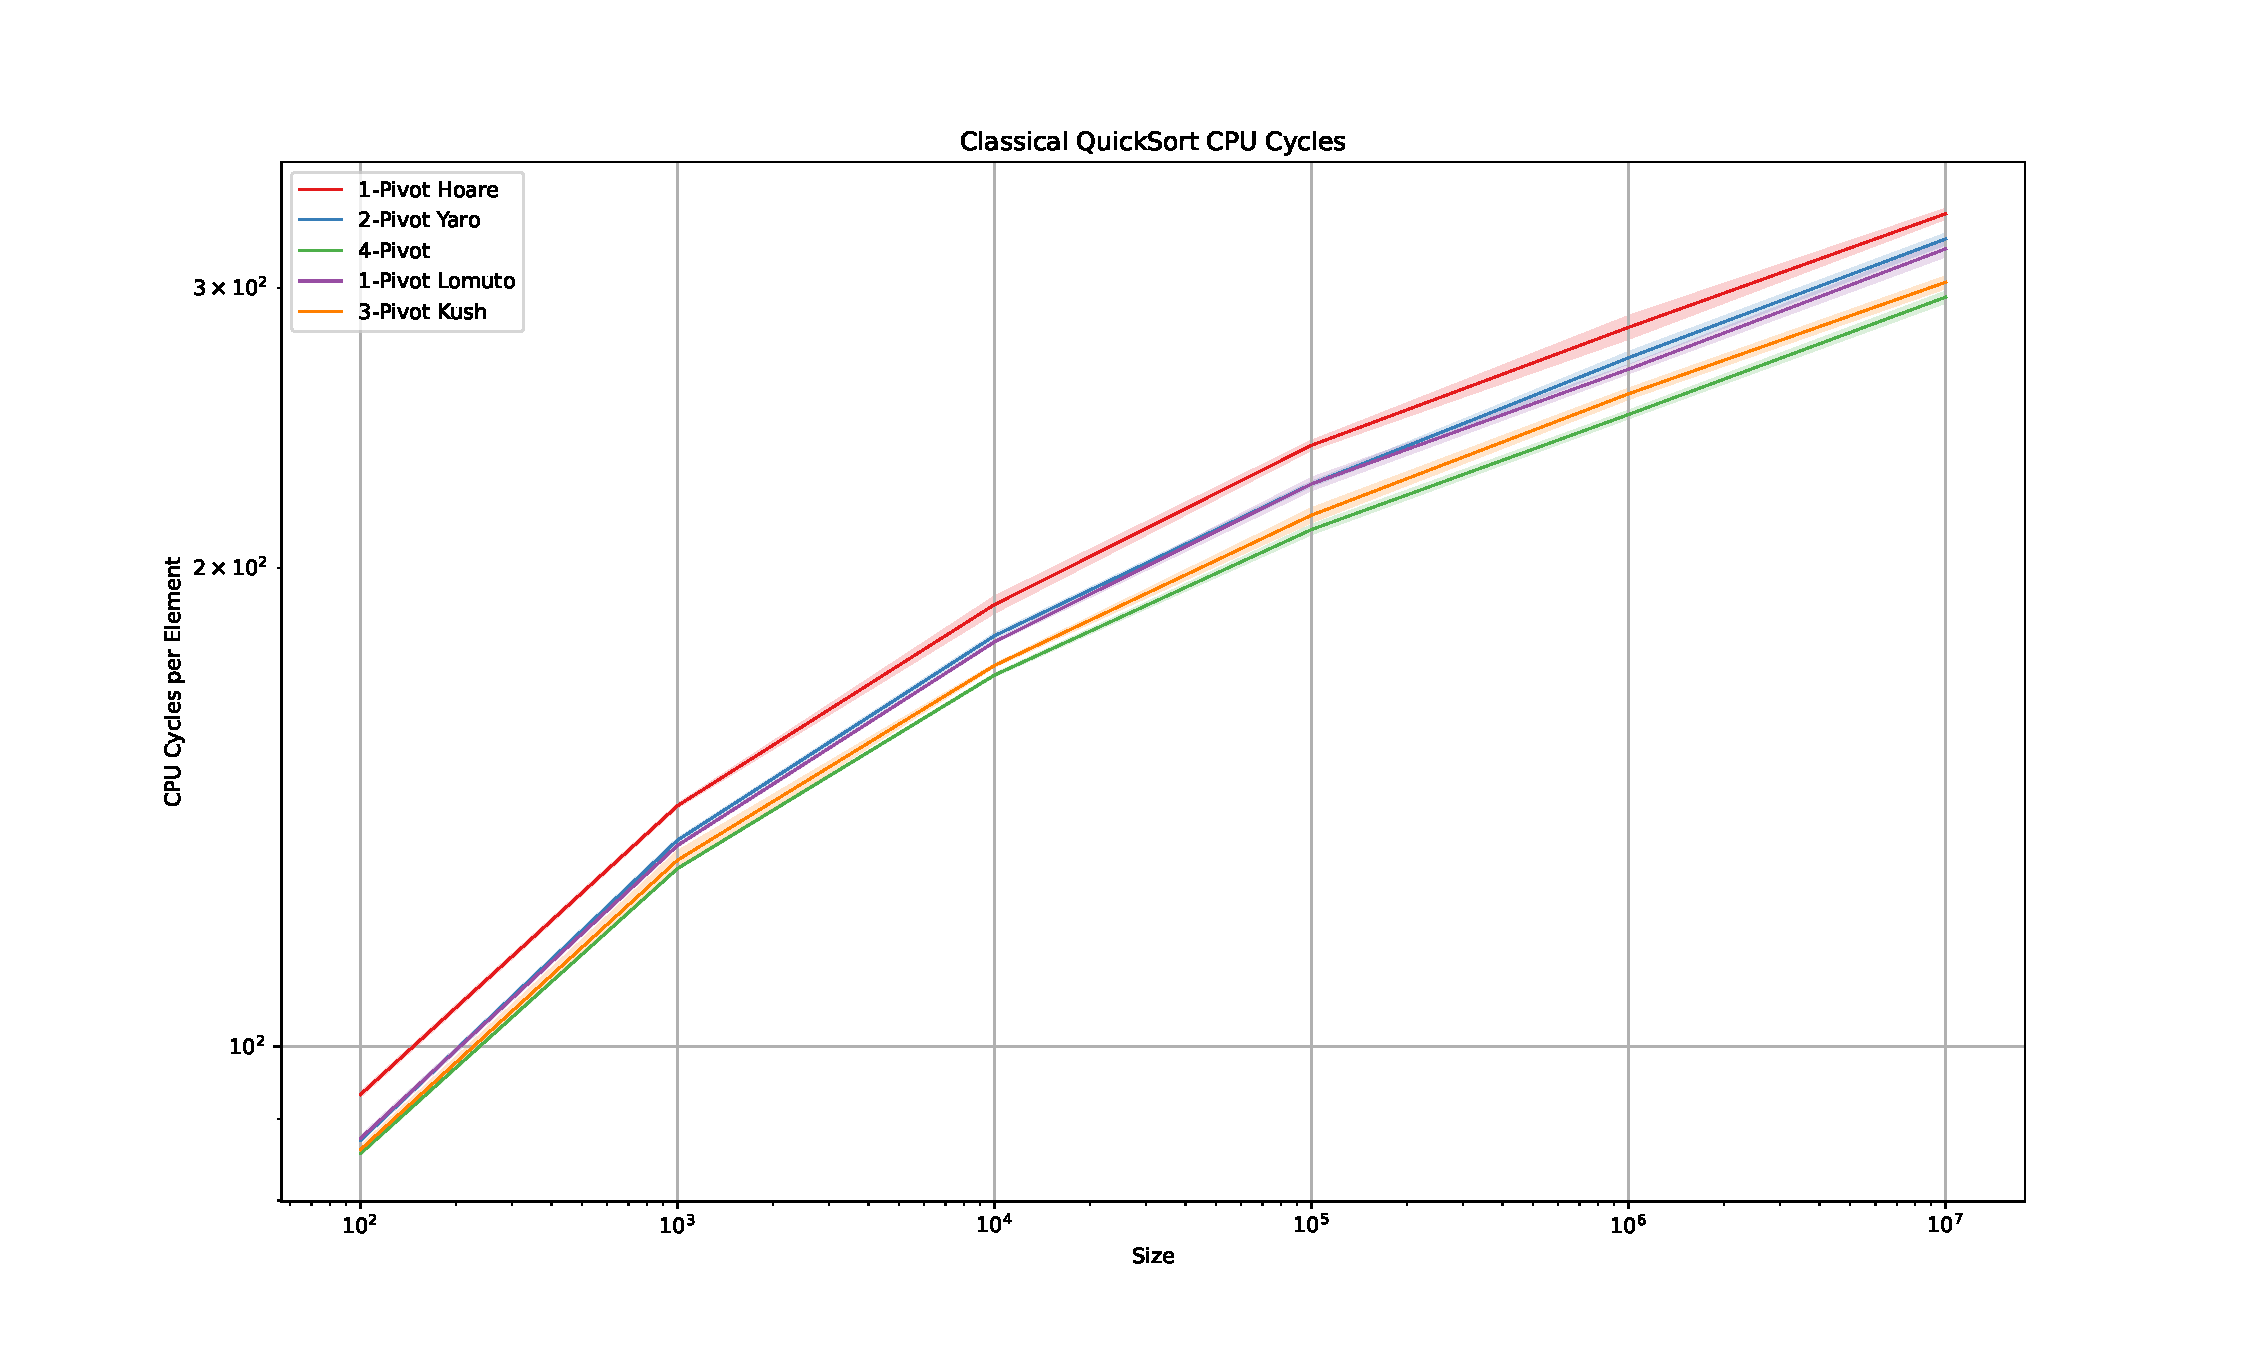
\includegraphics[width=1.5\textwidth]{Classical QuickSort CPU Cycles.pdf}
\end{figure}

Now it is time to deal with the total CPU cycles, the global trend is as the pivots increase, the number of CPU cycles falls.
But the 2-Pivot Yaroslavskiy's method exposed its weakness with respect to the 1-Pivot Lomuto's method. 

\begin{figure}[H]
    \hypertarget{fig:classicaltime}{}
    \caption{Classical QuickSort Time}
    \centering
    \hspace*{-0.27\textwidth}
    % \vspace*{+0.1\textheight}
    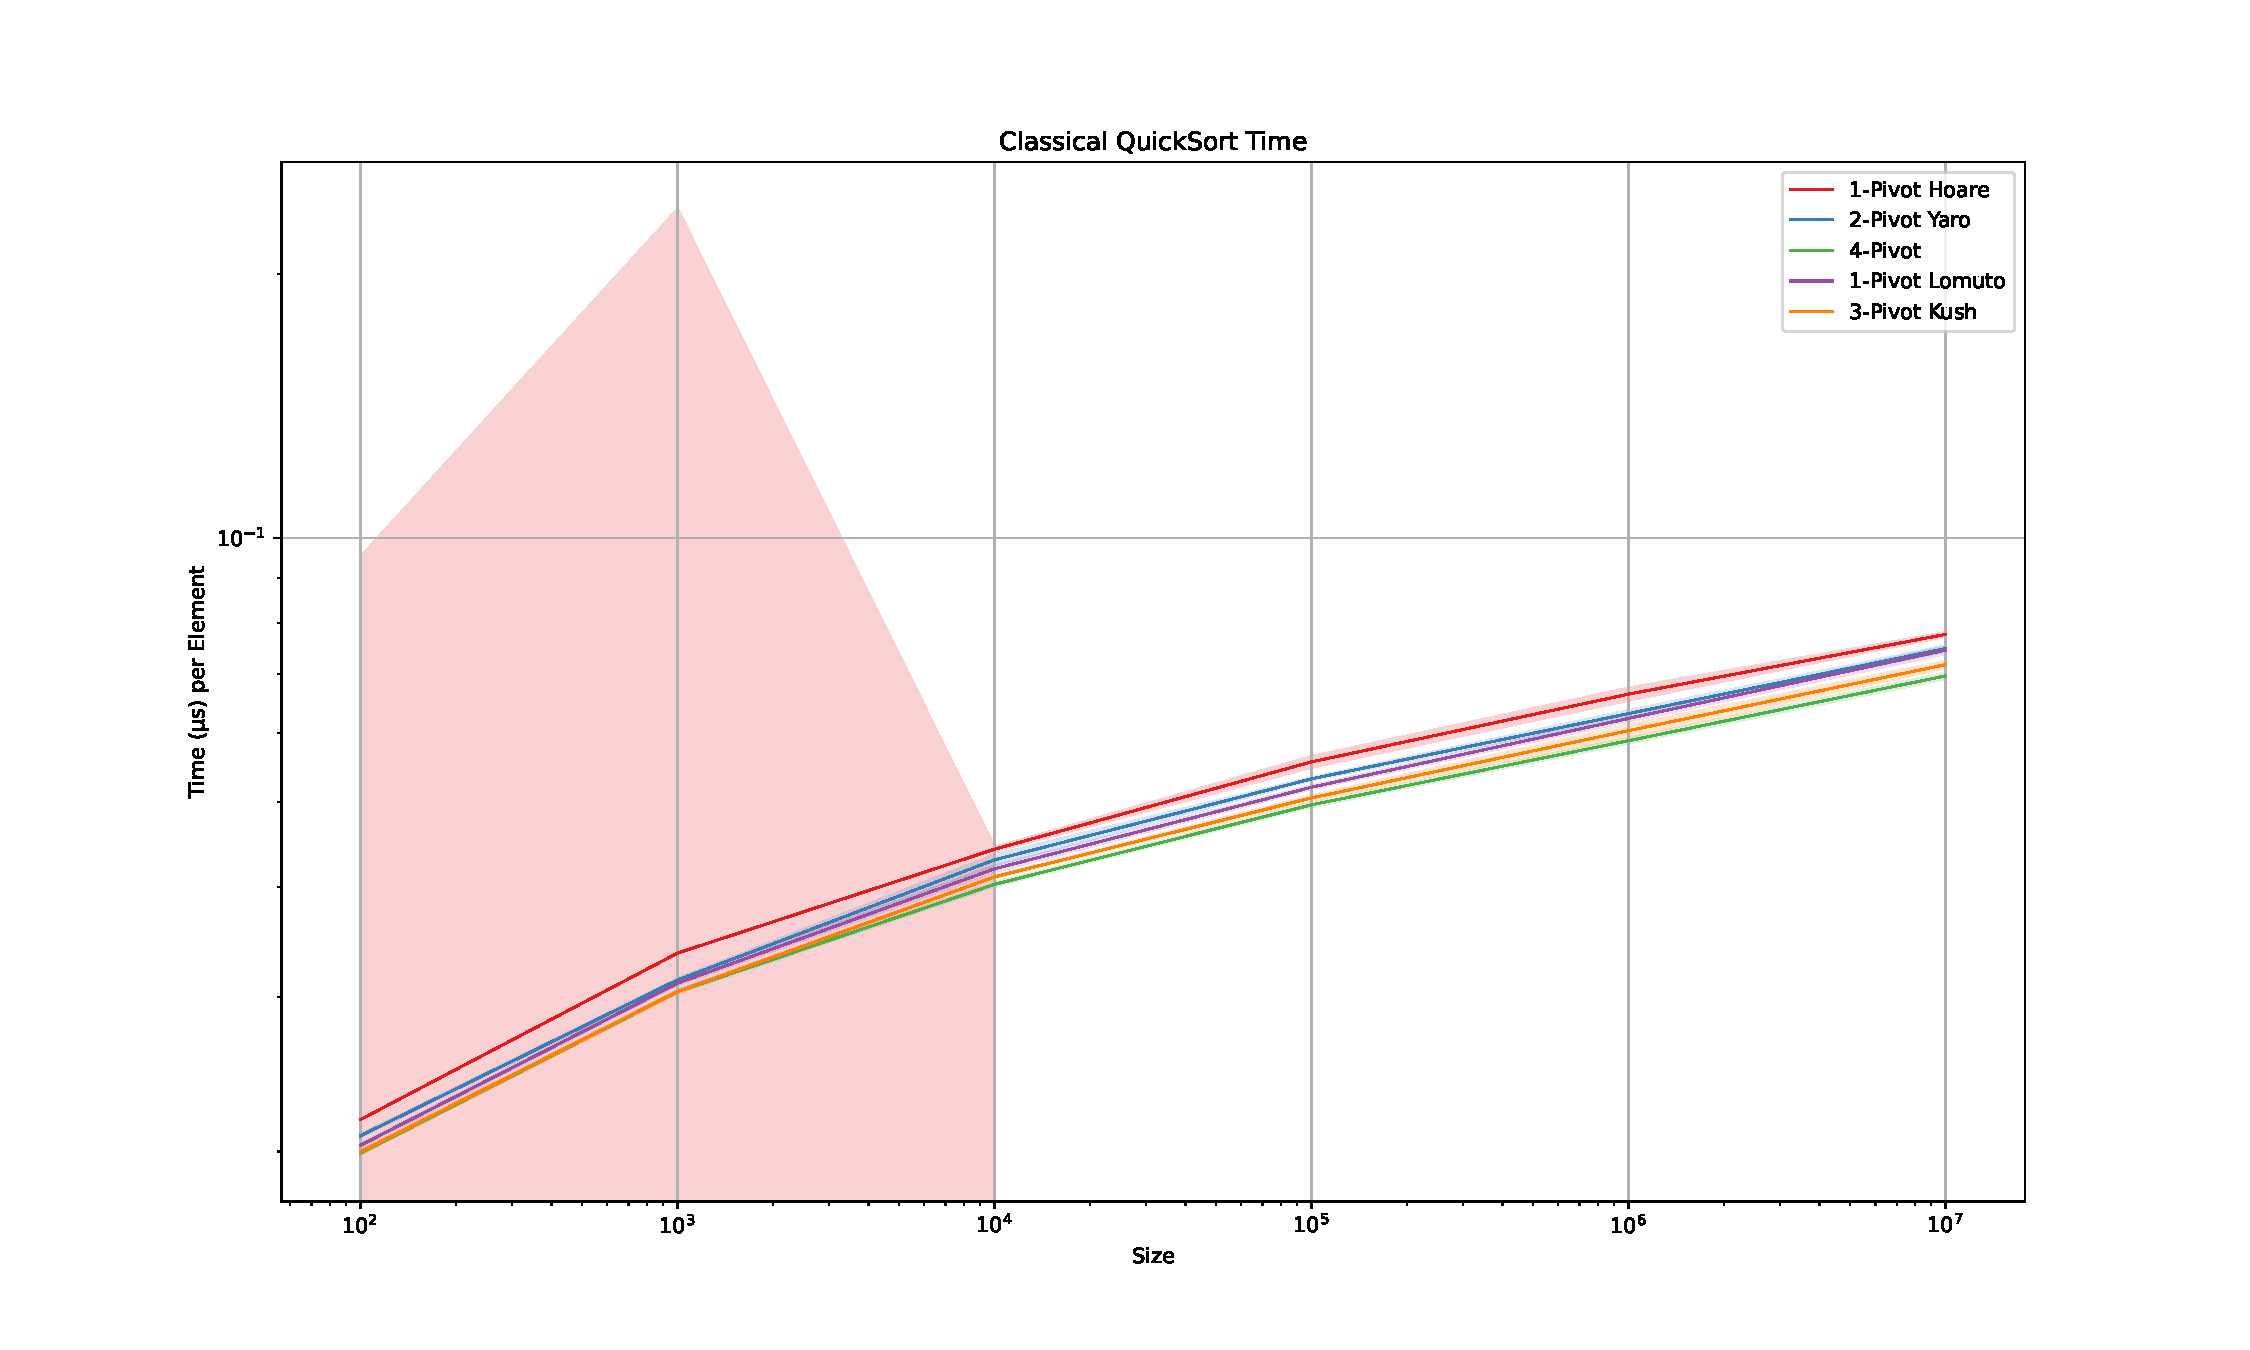
\includegraphics[width=1.5\textwidth]{Classical QuickSort Time.pdf}
\end{figure}

% A former analysis concerning the details of the overall costs and partitioning costs has been brought by Hennequin's thesis \cite{Hennequin} in terms of Multi-Pivot QuickSorts,
% where the author proved that if the average partitioning cost for $n$ elements is $a\cdot n + O(1)$ with a constant $a$, the overall cost then will be $\frac{6}{5}a\cdot n \ln n + \bigO{n}$.
% TODO: WTF does this mean? I need to understand this first before I can write it down.

Contrary to our expectations, 2-Pivot Yaroslavskiy's method was defeated by the 1-Pivot Lomuto's method in terms of runtime, even though it outperformed in the cache misses.
The running time does show the correlation with the branch misses while cache misses don't seem to have a significant impact, evidenced by Yaroslavskiy's method, who has lower cache misses but more cost time than Lomuto's method.
Similarly, despite of lower cache misses than Kushagra's 3-Pivot method, Yaroslavskiy's method still incurred significantly higher runtime for arrays with over 1 million elements.
This suggests that the past analysis on the cache misses have been constrained by array size, and perhaps the old CPU architecture's deficiency on handling large chunk of data flooding in and out of cache.

It brings to our attention that the testing CPU, R7 3700x, features a 16MB L3 cache, which is divided into two 8MB segments per CCD ($2 CCDs \times 8MB = 16MB$), with each segment serving 4 cores.
This limitation was later addressed in the Zen 3 architecture, R5 5600x for instance, where a unified L3 cache is shared across all cores, thanks to the high-performance ring buses that faciliate efficient cross-CCD communication that significantly reduce the latency.

The final running time also supports the exceptional cases mentioned above, indicating that cache misses don't necessarily have a direct impact on the final performance of the algorithm.
The 1-Pivot Hoare partition, characterized by 2 while loops scanning for the out-of-order elements on both sides, introduces extra overheads on branch misses and didn't manage to compete with other algorithms.
This could be the actual pain point that the 1-Pivot Hoare's method has to face, the branch misses appear to be the bottleneck, but we will soon find out the way to overcome it in the following sections.

What's enligntening is that the 4-Pivot method has the least amount of time, with both less branch misses and less cache misses than 3-Pivot, while the improvements are made in small steps, the overall performance is promising,
although how the 4-Pivot method has more predicted branches but less actual branch misses still requires further researches.

\begin{center}
\small
\begin{tabular}{ |c c | c | }
    \hline
    Time            & Size     & Mean         \\
    \hline
    2-Pivot Yaro    & 100000   & 5.3164 ms    \\
                    & 1000000  & 63.092 ms    \\
                    & 10000000 & 748.26 ms    \\

    \hline
    3-Pivot Kush    & 100000   & 5.0570 ms    \\
                    & 1000000  & 60.328 ms    \\
                    & 10000000 & 717.27 ms    \\
    \hline
    4-Pivot         & 100000   & 4.9661 ms    \\
                    & 1000000  & 58.758 ms    \\
                    & 10000000 & 696.42 ms    \\
    \hline
\end{tabular}
\end{center}

In conclusion, our experiments reveal unexpected nuances in algorithm performance comparisons, the 2-Pivot Yaroslavskiy's method has lower cache misses than 3-Pivot, least branch misses among multi-pivot variations but deficient performance on $10^7$ size of data, the 4-Pivot method has the least amount of time,
somewhat partially due to its favorable cache behavior, but more importantly, less branch misses in field experiments than predicted. The riddle between predicted and actual branch misses in the 4-Pivot method suggests new avenues for exploration and optimization.

% TODO: maybe talk about SSSSort as it uses 127 pivots, technically it is another variation of Multi-Pivot QuickSort, but it is not yet tested in this thesis.
% and it is really slow on many duplicates, but it is still worth mentioning.

% TODO: talk about some failed layouts that is way too complicated to implement, like 2 pivot hoare block partition.

% TODO: polish following paragraphs staring from here

With the help of my supervisor Dr. David Gregg I reached out to new layouts that might shift our perspectives on classical QuickSorts. Unfortunately they proved to be too complicated to implement or just not possible to be implemented by far.
One of the layouts is the 2 unknown segments for 2-Pivot QuickSort.

\begin{figure}[H]
    \hypertarget{fig:2pivotnewlayout}{}
    \caption{2-Pivot New Layout}
    \centering
    \hspace*{-0.27\textwidth}
    % \vspace*{+0.1\textheight}
    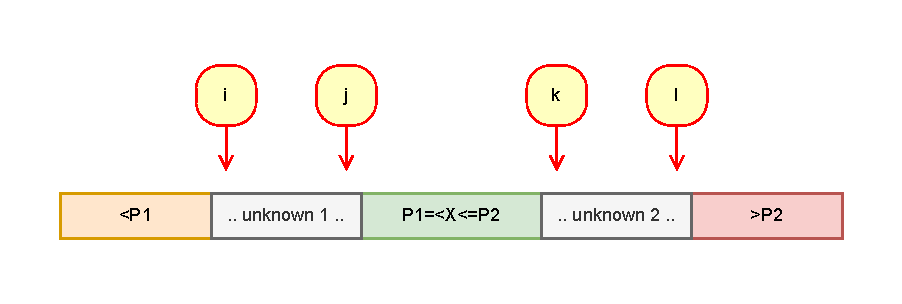
\includegraphics[width=1.5\textwidth]{2pivot_new_layout.drawio.pdf}
\end{figure}

Obviously, this will dramatically add the complexities to our algorithms when introducing one more unknown segment, which means 2 more unknown elements at the boundaries of the unknown region. Worst cases is, the comparison procedure will be consist of 4 if-else nested branches, each deciding the final destination of one of the 4 unknown elements at index $i, j, k, l$.
This could be a disaster for branch prediction, and the cache misses will be increased as well, as the elements are more likely to be swapped between the unknown regions, contributing the form of vicious cycle that will cause the performance degradation. This early exploration has been abandoned due to the complexity and the potential performance issues it might bring.

While searching for the solutions to the branch misses, I have found that BlockQuickSort could refresh us with a new vision of partitioning, it's easily adaptable to most of the partition methods and its direct impact on the performance is beyond amazing
according to what has been observed in the tests below.

\begin{figure}[H]
    \hypertarget{fig:blockbranchmiss}{}
    \caption{Block QuickSort Branch Misses}
    \centering
    \hspace*{-0.27\textwidth}
    % \vspace*{+0.1\textheight}
    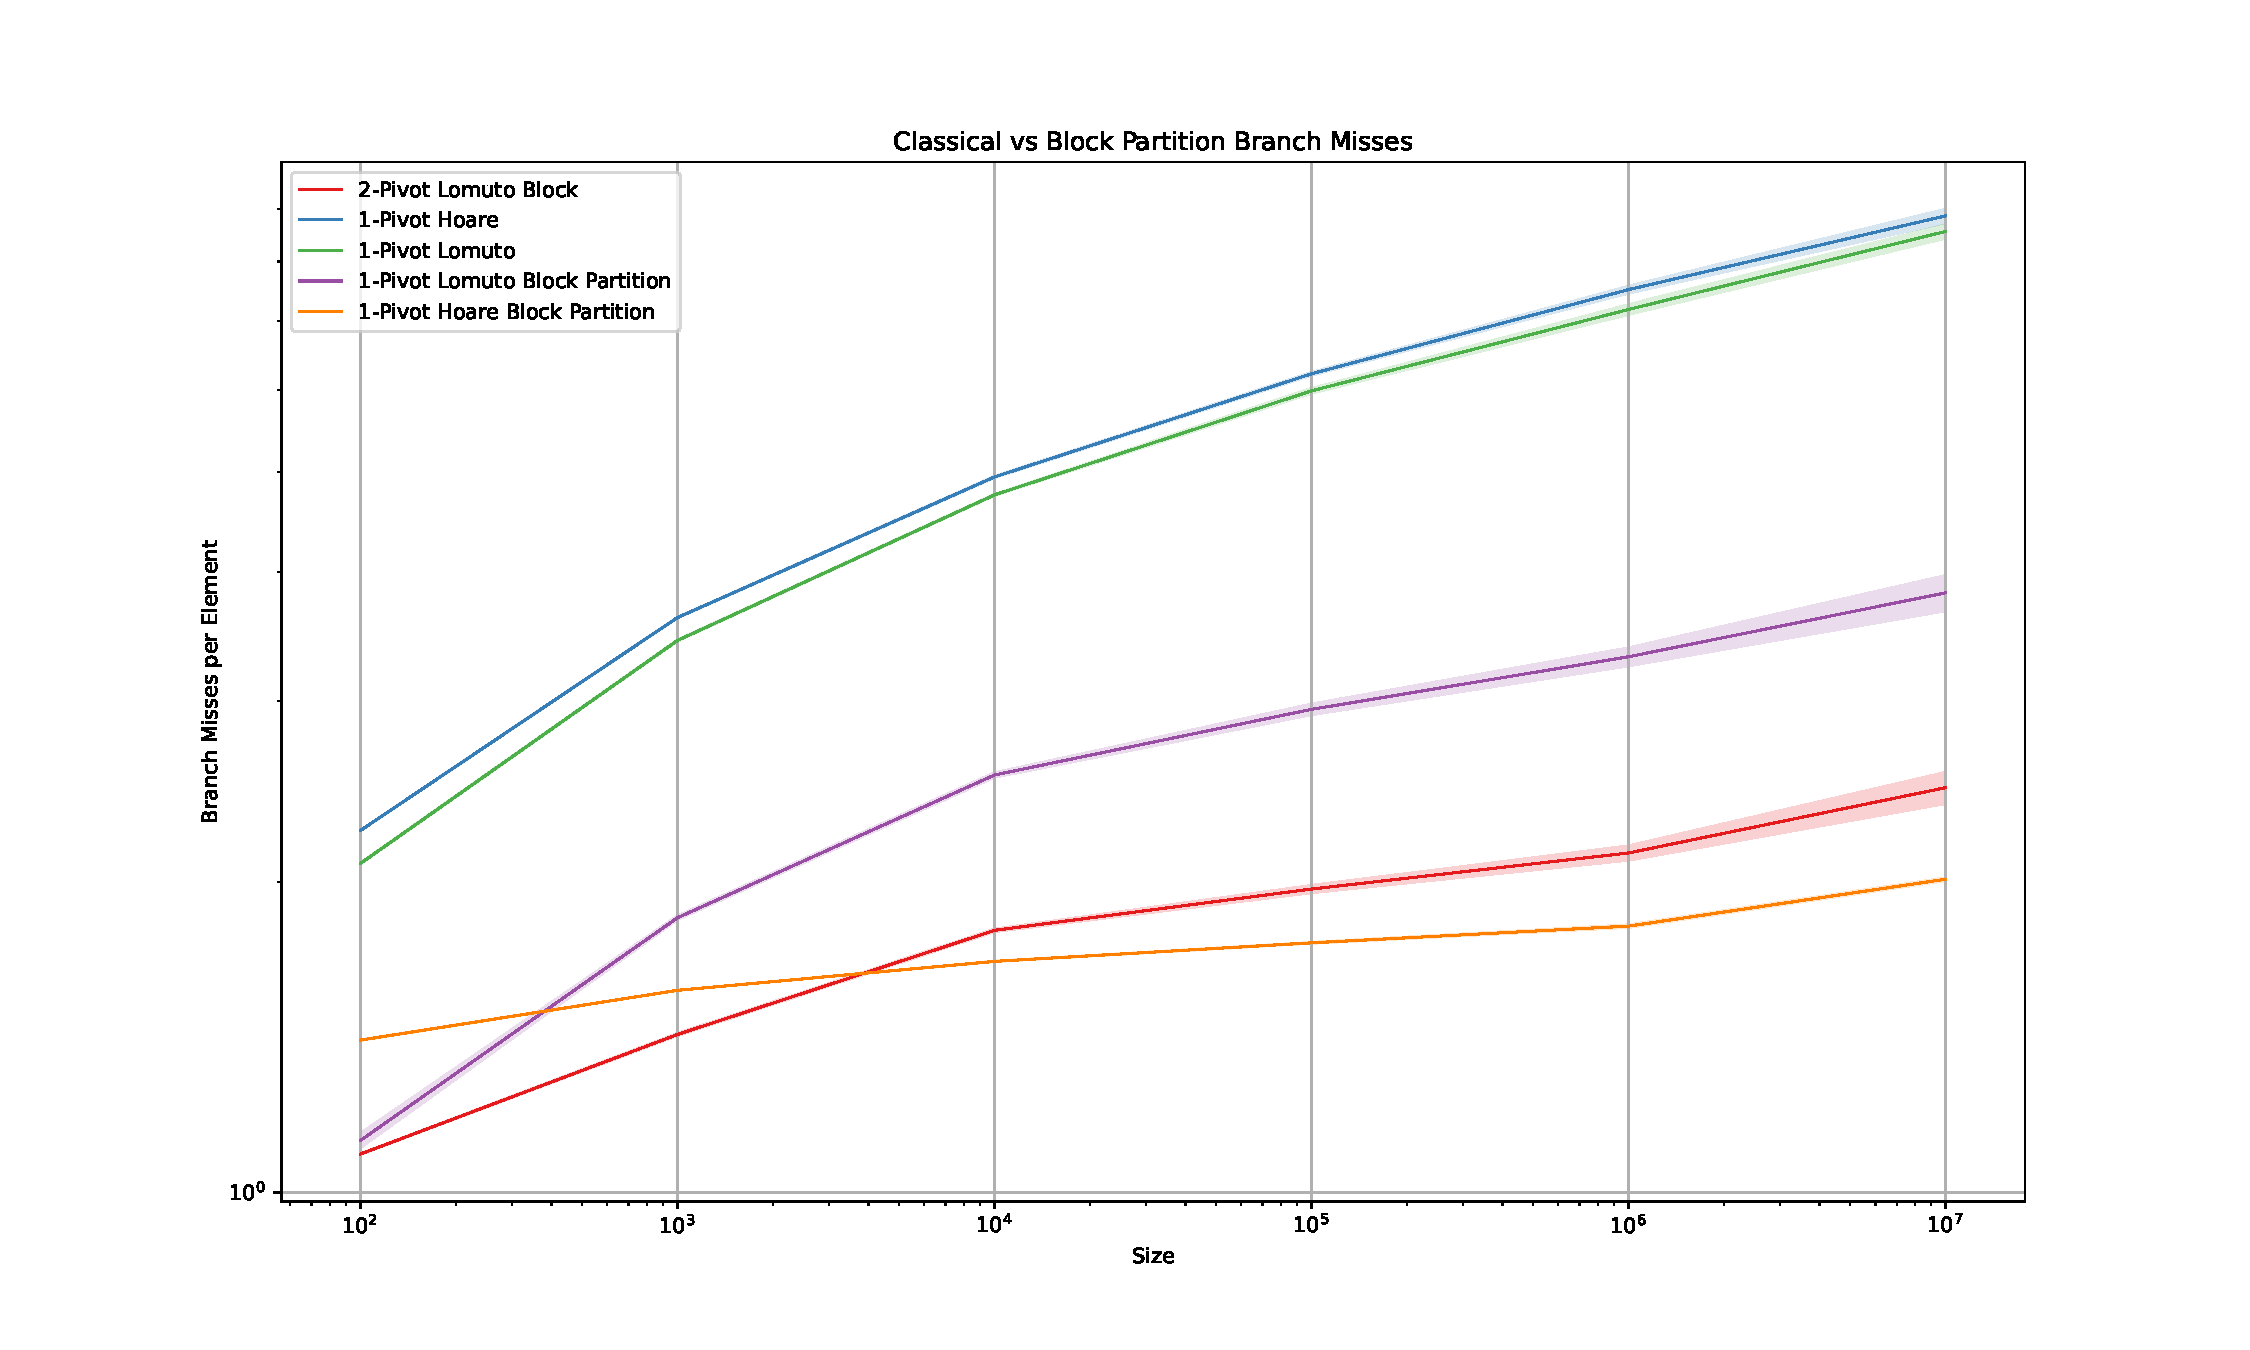
\includegraphics[width=1.5\textwidth]{Classical vs Block Partition Branch Misses.pdf}
\end{figure}

\begin{center}
\small
\begin{tabular}{ |c c | c | }
    \hline
    Branch Misses   & Size     & Mean         \\
    \hline
    1-Pivot Hoare   & 100000   & 622681.46    \\
                    & 1000000  & 7514512.06   \\
                    & 10000000 & 88601386.65  \\
    \hline
1-Pivot Block Partition & 100000   & 174650.07    \\
                    & 1000000  & 1813011.99   \\
                    & 10000000 & 20131908.65  \\
    \hline
    1-Pivot Lomuto  & 100000   & 599369.59    \\
                    & 1000000  & 7188431.33   \\
                    & 10000000 & 85572728.60  \\
    \hline
1-Pivot Block Partition & 100000   & 294244.78    \\
                    & 1000000  & 3309146.60   \\
                    & 10000000 & 38173447.65  \\
    \hline
2-Pivot Lomuto Block& 100000   & 196951.71    \\
                    & 1000000  & 2134863.07   \\
                    & 10000000 & 24700025.80  \\
    \hline
\end{tabular}
\end{center}

With the help of Block Partition together with branchless comparisons and branchless additions on counters, we reduced about 70\% of the branch misses in the 1-Pivot Hoare's method, and 40\% in the 1-Pivot Lomuto's method. These results will only increase as the size of the array grows.
On gigantic arrays of size 10 million, we achieved 77\% and 55\% branch miss reductions respectively as a result. \hyperlink{FullTables}{Full tables} of detailed statistics could be found in the final appendix. That's a huge success so far, though it doesn't show superior performance on smaller arrays, but the average branch misses barely even increase as the size grows exponentially.

\begin{figure}[H]
    \hypertarget{fig:blockcachemiss}{}
    \caption{Block QuickSort Cache Misses}
    \centering
    \hspace*{-0.27\textwidth}
    % \vspace*{+0.1\textheight}
    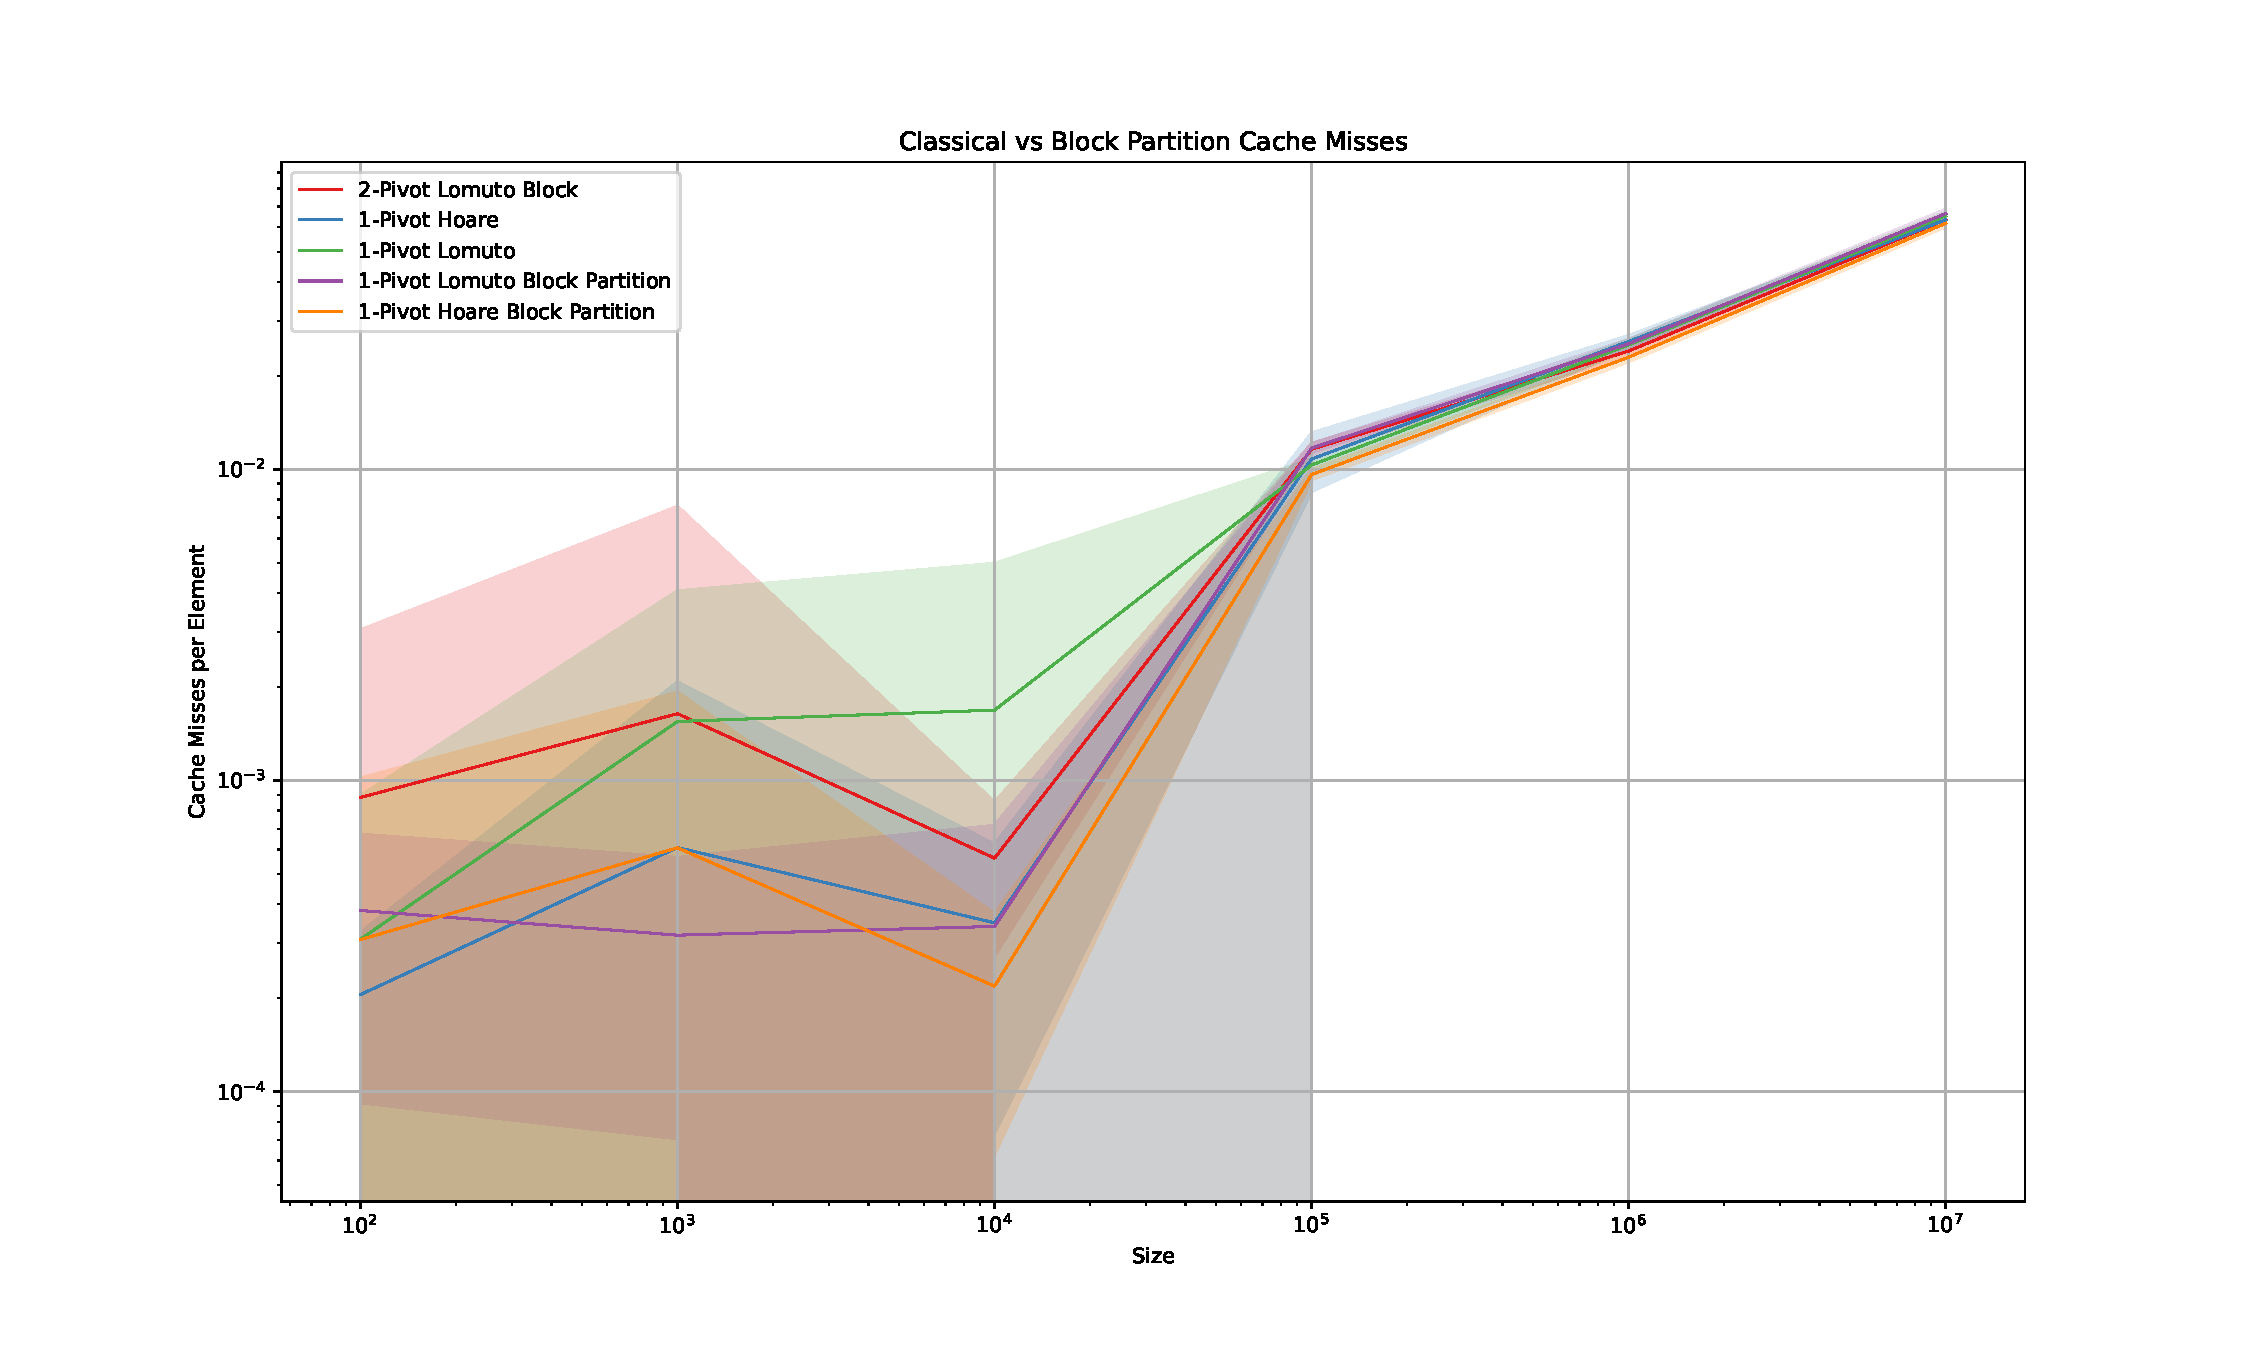
\includegraphics[width=1.5\textwidth]{Classical vs Block Partition Cache Misses.pdf}
\end{figure}

Again to our surprise, the changes in cache miss isn't as obvious as the branch misses, the tiny improvements on Hoare's Block Partition and 2-Pivot Lomuto's Block Partition seem to be only exceptions.
Considering the traditional partition schemes only require very small number of constant size, comparing to the large chunk of memory required by the Block Partition, the Block Partition's revision on Lomuto's method adds more cache misses instead.
But as we observe the CPU instructions count and the time cost, we will find out that the Block Partition's method is still the best choice for the 1-Pivot Hoare's method, and the 2-Pivot Lomuto's method.

\begin{figure}[H]
    \hypertarget{fig:blockcpucycles}{}
    \caption{Block QuickSort CPU Cycles}
    \centering
    \hspace*{-0.27\textwidth}
    % \vspace*{+0.1\textheight}
    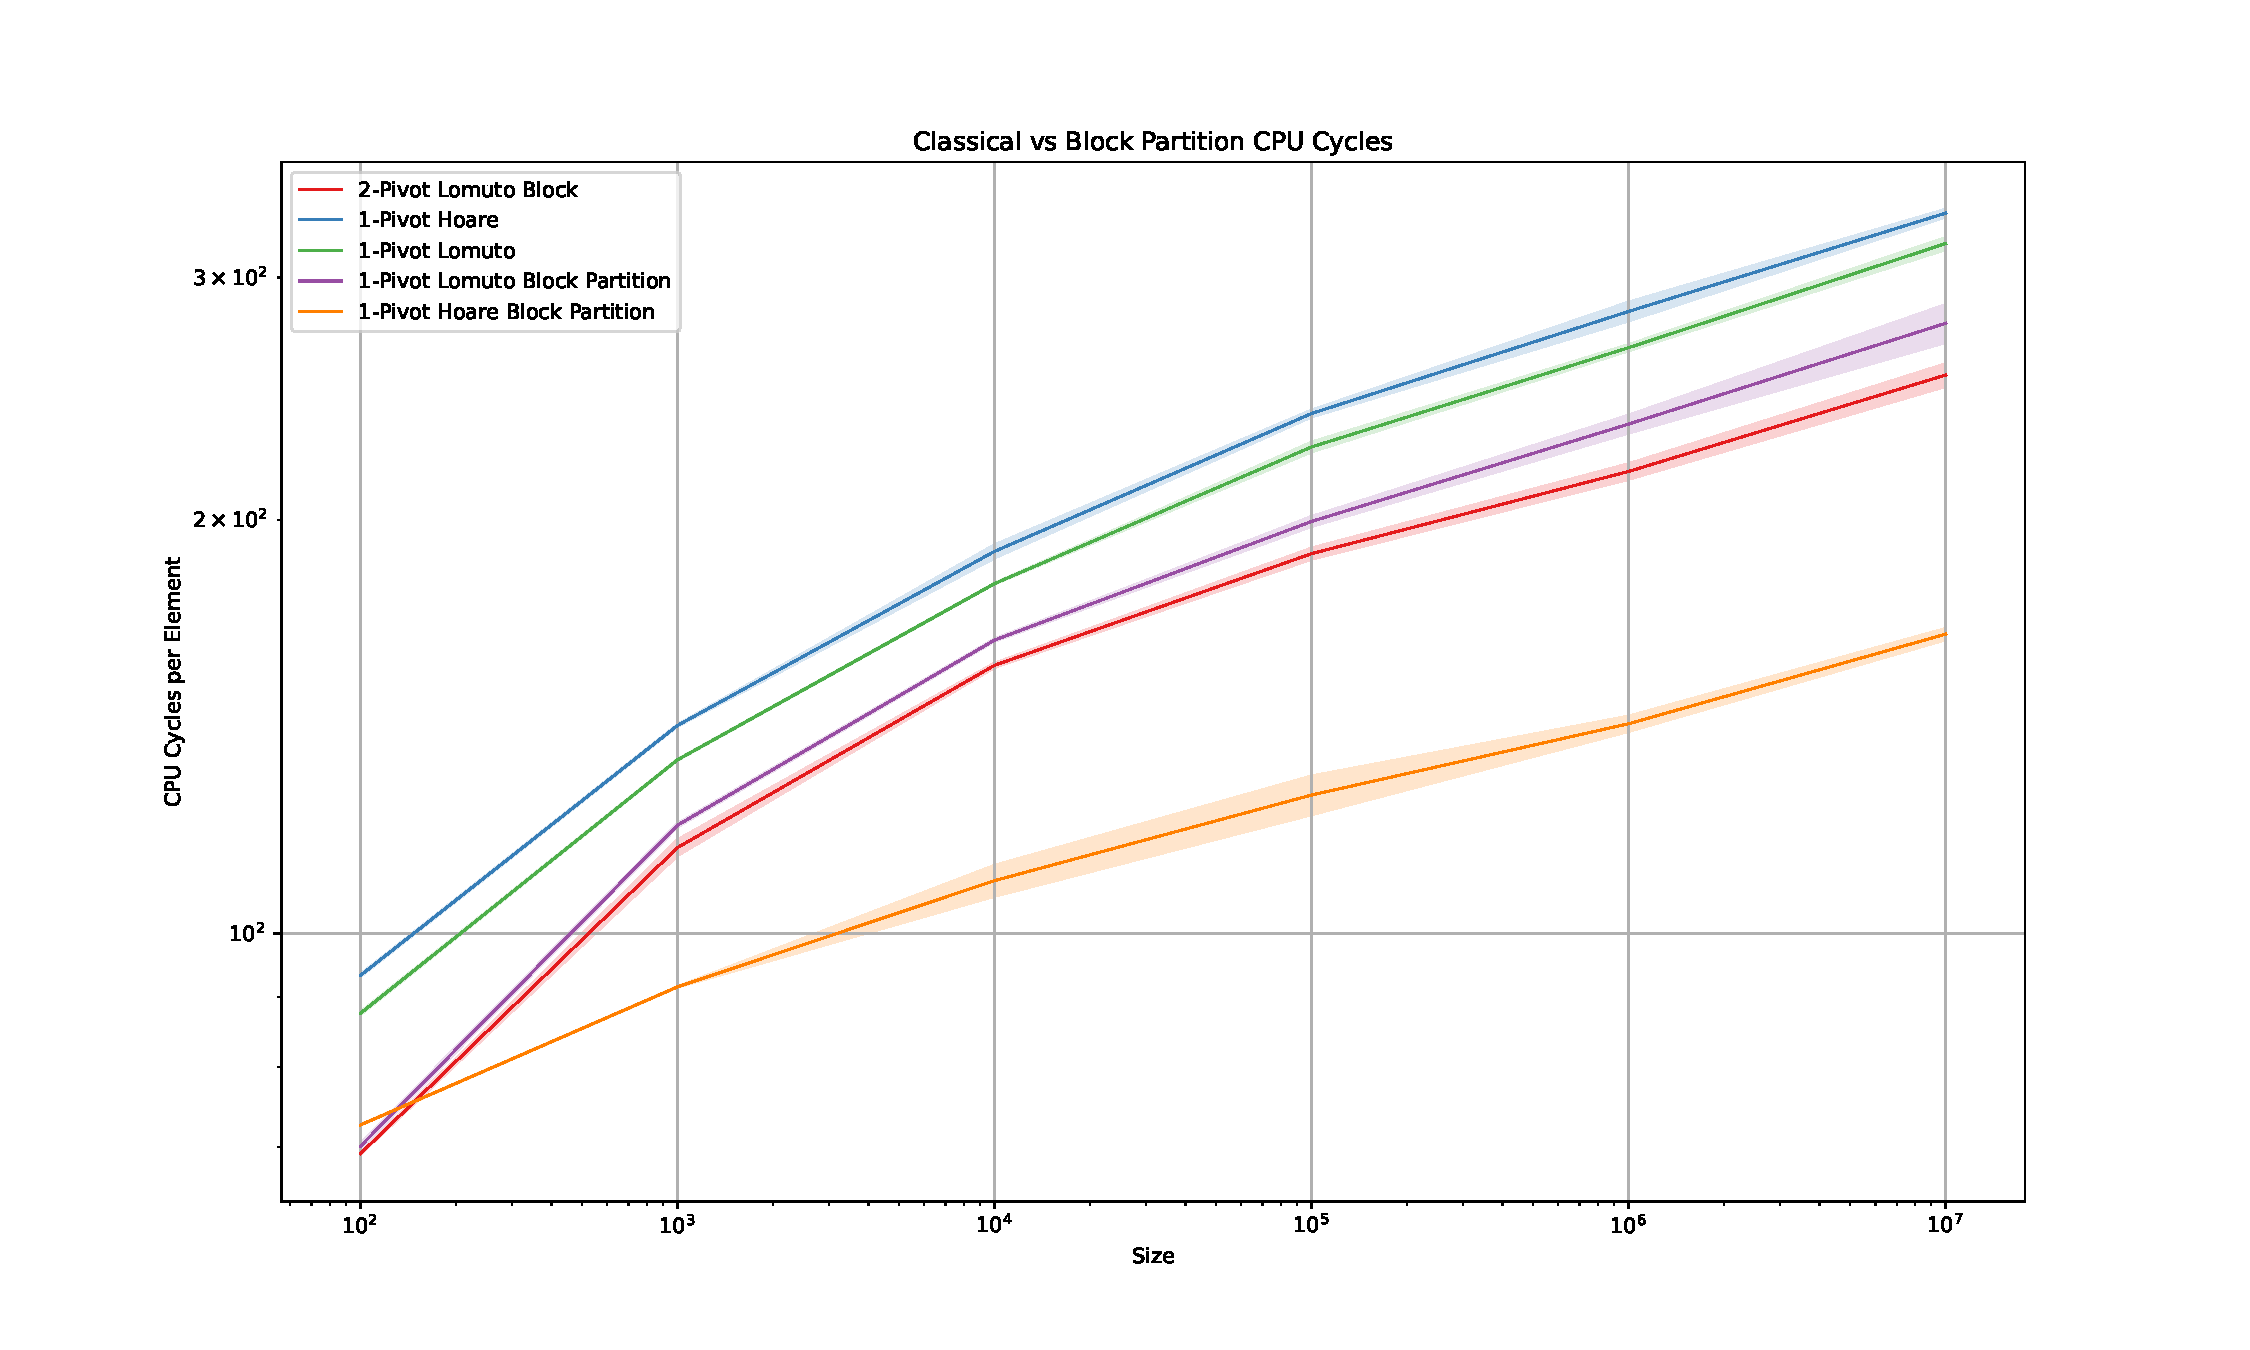
\includegraphics[width=1.5\textwidth]{Classical vs Block Partition CPU Cycles.pdf}
\end{figure}

It seems the Hoare's Block Partition has the most significant improvements on the CPU cycles, with about half of the reductions on total cycles.
The block partition doesn't seem to improve much with the Lomuto's scheme, which is still a mystery to me together with its dramatic standard deviation, but the 2-Pivot Lomuto's Block Partition has a decent amount of improvements.
Still, the cache misses for small arrays seem completely random, so are the standard deviations. There seems no way that we could analyse these results. But the time cost will give us a clear answer.

\begin{figure}[H]
    \hypertarget{fig:blocktime}{}
    \caption{Block QuickSort Time}
    \centering
    \hspace*{-0.27\textwidth}
    % \vspace*{+0.1\textheight}
    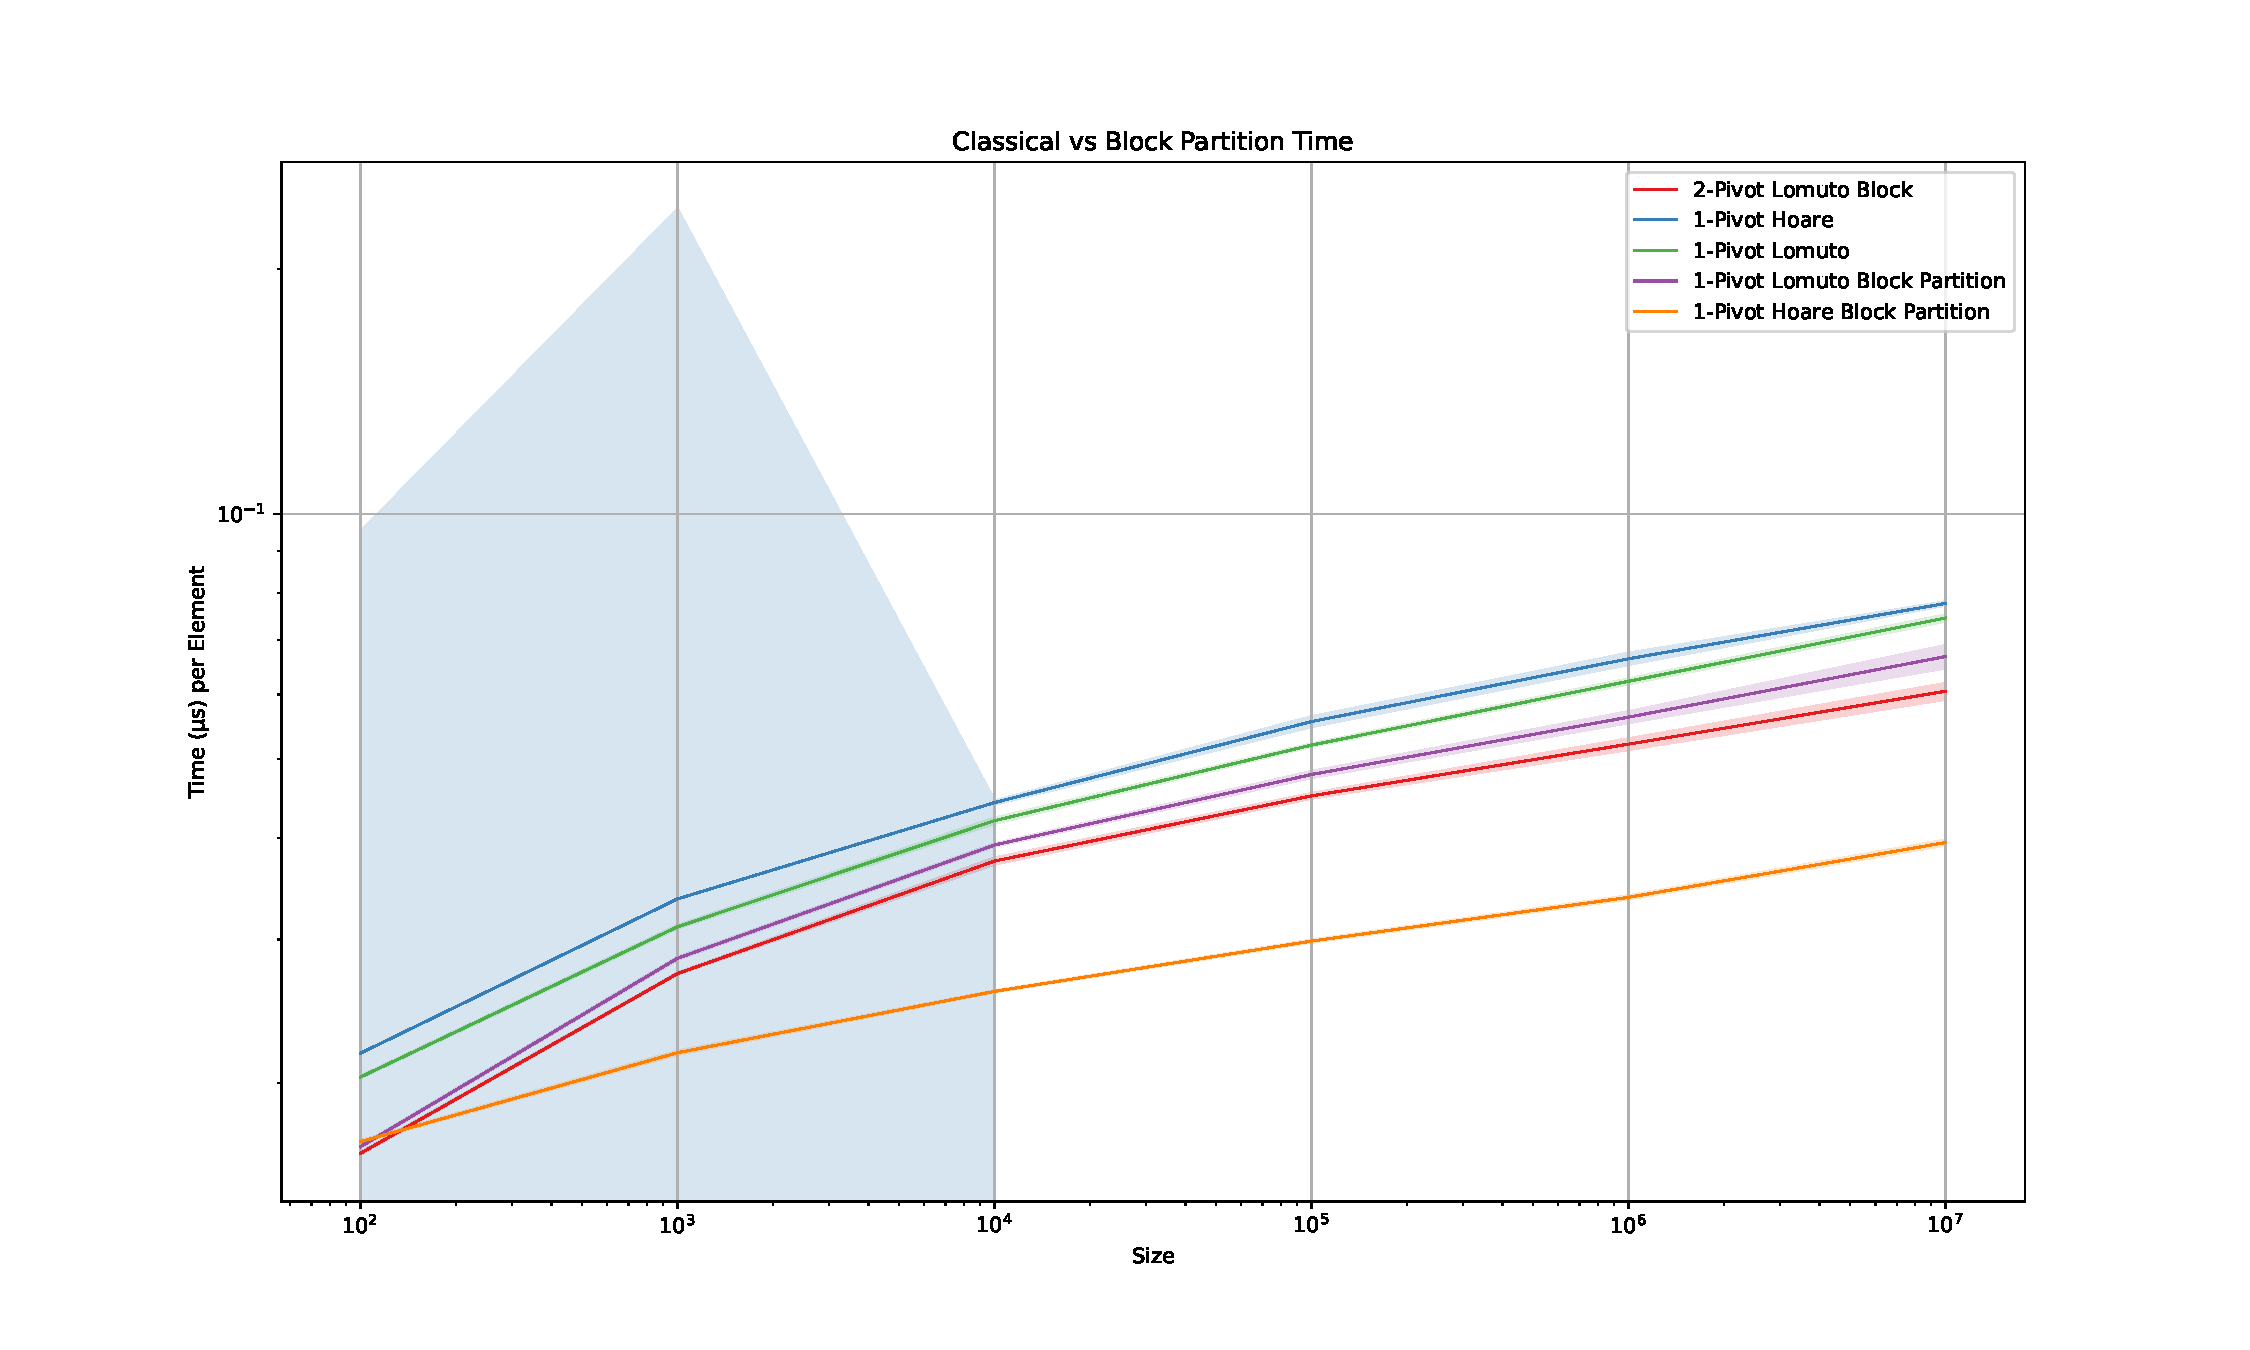
\includegraphics[width=1.5\textwidth]{Classical vs Block Partition Time.pdf}
\end{figure}

The most intriguing result has been given by the 1-Pivot Hoare' BlockQuickSort variation with least amount of time cost, nearly the half as the original, as a result of less than 3\% improvement on cache misses and approximately 70\% improvement on branch misses.
It is already of much progress I would have to say, but the 2-Pivot Lomuto's BlockQuickSort variation also has a decent amount of improvements, with up to 18\% less time cost than the original.
The former example has proven a success, but future works will also be carried out to improve the cache misses, even though there exists very limited things we could do,
the modern CPU architecture has already done a great job on the overall cache hit rate, which can be supported by the cachegrind tests that all the tested algorithms have around less than 10\% cache misses.
Although this won't be the deterministic evidence to say that the cache misses are not the bottleneck, but it is still a good sign that the cache misses are not the main issue that we have to deal with.

% TODO: talk about pivot selection and skewed pivot selection like page 11 of block quick sort paper.
The tests above are carried out using constant pivot selection method, choosing half start and half end of the array as the pivots as the most common practice goes,
but as mentioned earlier in the preliminaries part \hyperlink{ref:AnalysisOfBranchMissesInQuickSort}{`}, the pivot selection is a crucial part of the QuickSort algorithm, and the skewed pivot selection, anti-tuitionally as it seems, could bring better performance than the random pivot selection.
It doesn't bring us to the conclusion that the skewed pivot selection is always better other methods, even it makes sense to a static branch predictor where it assumes all branches will follow the correct majority path, for instance, if our skewed pivot could divide the array into $x\%$ and $(100-x)\%$ parts, the branch predictor will always predict the $max(x\%, 100-x\%)$ path,
we can use less time at current stage to finish the partitioning process, but the imbalanced partitions will pose future challenges to maintain the efficiency of overall algorithm. Luckily, skewed pivot always proves unnecessary in the BlockQuickSort, free from the concerns on branch misses' costs in the experiments of \cite{BlockQuickSort}. With skew factor 2 (the middlest element is chosen as the pivot), the BlockQuickSort has the least amount of time cost, and larger skew factors will only increase the runtime. Skew factor of 6 appeared to have the best performance in the experiments for classical QuickSorts as a balance between the stalls caused by branch misses and total CPU Instructions.

% TODO: 2 pivot lomuto's block partition is faster than the classical quicksort but slower than the 1 pivot hoare's block partition, why?
The 2-Pivot Lomuto's Block Partition has less branch misses for smaller arrays, but fail to compete as the size extends, as the duplicated swaps have been enlarged when the size of the array grows, 
Lacking as a key feature to Lomuto's block scheme is the cyclic swaps that relief a lot of duplicated swaps and constant cache to the temp variable. This method has adapted well to the Hoare's scheme, for it starts on both ends and the duplicated swaps are less likely to happen as long as mis-placed elements are spotted on both sides, a prerequisite for the cyclic swaps to take place.
The cyclic swaps are not only reducing the duplicated swaps, but also reducing the cache misses by the help of write-back policy. The 2-Pivot Lomuto's Block Partition has failed to adapt to the massive cyclic swaps that eliminates the biggest headache of small swaps' costs on frequently changed temp variable, plus the duplicated swaps are not reduced, but amplified, which might be the meat of the issue for the performance degradation compared with Hoare's block partition. % TODO: is this the real reason? I need to check the code again.
% TODO: talk about the new trial layout of block quick sort, 2 pivots and lomuto, and why it is slower
Mimicing the layout of Lomuto's Block Partition, I implemented another 2-Pivots Lomuto's Block Partition which requires only one phase of rearranging, but with more rotate-n moves to shift elements to their correct partitions. This could introduce more complexity as in a chaotic block with 2 types of items less than Pivot 1 or greater than Pivot 1 but less than Pivot 2,
simply dumping their offsets to the correct partitions regardless will not work, for in each step we have to deal with smaller offset first to make sure our algorithm behaves the same as the classical version which scans the array in one-way order, but this extra min() operation could be a huge drawback for this scheme.
Results for this is even slower than the classical QuickSort, and it is not recommended to be used in practice, only for academic purposes instead of industrial applications.
\begin{figure}[H]
    \hypertarget{fig:newblock}{}
    \caption{Block QuickSort New 2-Pivot Lomuto}
    \centering
    \hspace*{-0.27\textwidth}
    % \vspace*{+0.1\textheight}
    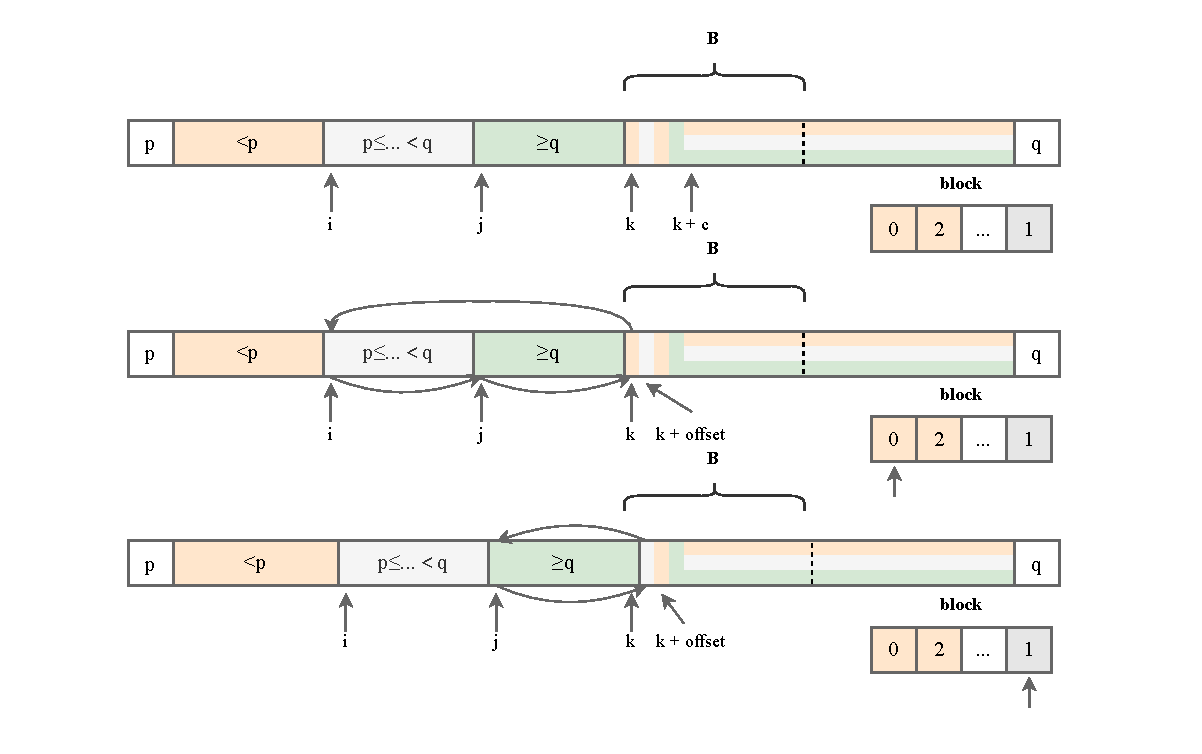
\includegraphics[width=1.5\textwidth]{new_lomuto_block.drawio.pdf}
\end{figure}
The cache misses also suffer from the new layout, constantly swapping side to read and compare the next minium offset also poses a challenge to the spatial locality of cache,
causing the general time cost being also higher than the classical QuickSort. In my fuzzy tests of cachegrind \hyperlink{cachegrindresult}, the data read (Dr) rate 28.98\% and data write (Dw) rate 19.41\% all rank the top, and are both much higher than the classical QuickSort even though it has low cache misses.
My assumption would be these constant memory accesses are caused by the cache write-back policy due to inconsistent spatial locality, though the actual relationship is yet to be confirmed by further tests in the future.
It reveals from another perspective that the block partition is restricted by the number of pivots, as the experiments in this thesis only shows that the the pattern of comparing with one pivot in one pass is the only way to go, otherwise, like the new layout illustrated above, if we get too greedy to compare with 2 pivots simultaneously,
the offsets have to be stored in separated chunks and it will introduce the memory accesses as the most expensive overheads that stall the CPU. This puts forward another trade-off between the number of pivots and the block partition, and it is not yet clear how to leverage the best of both worlds.
The BlockQuickSort is still in its infancy, despite the fact that PDQSort proves a great success in the real-world applications, and the future works will be carried out to explore more possibilities and to find more optimal layout for the BlockQuickSort.
As to the new layout, for your interest the detailed statistics will be attached in the appendix section.

% TODO: another layout, swap < P1 to the left and swap < P2 to the right. Is it worth trying?

% TODO: talk about the sorting functions exported to python by ffi
For the sake of convenience, the sorting functions are exported to Python using the Foreign Function Interface (FFI) provided by PyO3, which is a safe and easy way to call Rust functions from Python.
The sorting functions are then tested on the same machine with the same environment with supported types 32 bits IEEE-754 floats and unsigned 32 bits integers. The original Rust results are provided in the appendix in fully elaborated \hyperlink{FullTables}{tables}. The Python results are consistent with the Rust tests, reliable and stable.
Only extra overhead would be the Python interpreter and ffi calls, which is not significant in this case, and is negligible.
% % % % % % % % % % % % % % % % % % % % % % % % % % % % % %

\section{Full Tables}
\hypertarget{FullTables}{}
\begin{center}
    \small
    \begin{tabular}{ |c c | c c c| }
        \hline
        Branch Misses   & Size     & Mean           & SD            & Median \\
        \hline
        1-Pivot Hoare   & 100      & 224.4847       & 0.0588        & 224.4906 \\
                        & 1000     & 3612.1521      & 2.2119        & 3612.3146 \\
                        & 10000    & 49451.5958     & 72.9468       & 49464.5783 \\
                        & 100000   & 622681.4604    & 1879.7192     & 622662.0813 \\
                        & 1000000  & 7514512.0625   & 57015.6085    & 7528135.1250 \\
                        & 10000000 & 88601386.6500  & 1316610.4428  & 88910896.5000 \\
        Block Partition & 100      & 140.5428       & 0.0876        & 140.5400 \\
                        & 1000     & 1570.7223      & 0.3938        & 1570.6199 \\
                        & 10000    & 16756.4235     & 7.9552        & 16757.5304 \\
                        & 100000   & 174650.0671    & 156.4744      & 174665.2439 \\
                        & 1000000  & 1813011.9915   & 5043.7407     & 1811789.7762 \\
                        & 10000000 & 20131908.6500  & 59866.7898    & 20134795.0000 \\
        \hline
        1-Pivot Lomuto  & 100      & 208.5500       & 0.2674        & 208.4572 \\
                        & 1000     & 3431.9977      & 4.9888        & 3432.6774 \\
                        & 10000    & 47510.1674     & 62.4065       & 47492.9219 \\
                        & 100000   & 599369.5910    & 3094.0668     & 599127.2778 \\
                        & 1000000  & 7188431.3250   & 77244.2181    & 7204133.7500 \\
                        & 10000000 & 85572728.6000  & 1273266.3095  & 85589444.5000 \\
        Block Partition & 100      & 112.3253       & 1.7694        & 112.7843 \\
                        & 1000     & 1847.2526      & 6.8858        & 1570.6199 \\
                        & 10000    & 25410.1772     & 123.7813      & 25350.7255 \\
                        & 100000   & 294244.7788    & 3465.6995     & 294878.4121 \\
                        & 1000000  & 3309146.6000   & 66124.1202    & 3313478.8000 \\
                        & 10000000 & 38173447.6500  & 1498913.4243  & 37931268.5000 \\
        \hline
        2-Pivot Yaro    & 100      & 218.6639       & 0.0935        & 218.6437 \\
                        & 1000     & 3629.7245      & 1.7137        & 3630.2813 \\
                        & 10000    & 50301.2096     & 38.3586       & 50300.6213 \\
                        & 100000   & 635045.2987    & 2126.8544     & 634416.1873 \\
                        & 1000000  & 7624533.4500   & 45160.5385    & 7614424.8750 \\
                        & 10000000 & 90144952.0000  & 955908.5187   & 90243746.5000 \\
        Lomuto Block    & 100      & 108.9624       & 0.0537        & 108.9703 \\
                        & 1000     & 1423.2516      & 3.1800        & 1422.2247 \\
                        & 10000    & 17959.2518     & 49.0859       & 17951.8464 \\
                        & 100000   & 196951.7141    & 1583.5204     & 197172.6696 \\
                        & 1000000  & 2134863.0700   & 33965.1267    & 2119311.9000 \\
                        & 10000000 & 24700025.8000  & 856684.2381   & 24551996.5000 \\
        \hline
        3-Pivot Kush    & 100      & 231.0457       & 0.0996        & 231.0266 \\
                        & 1000     & 3828.0046      & 1.7692        & 3827.5547 \\
                        & 10000    & 52692.9469     & 57.0170       & 52699.8674 \\
                        & 100000   & 660656.7803    & 2410.3154     & 660486.3048 \\
                        & 1000000  & 7881473.7500   & 55041.5020    & 7885420.7000 \\
                        & 10000000 & 93039500.9000  & 1138513.6270  & 93254088.5000 \\
        \hline
        4-Pivot         & 100      & 233.3581       & 0.1961        & 233.3429 \\
                        & 1000     & 3847.1970      & 1.7934        & 3847.1812 \\
                        & 10000    & 52466.7069     & 69.7884       & 52466.1749 \\
                        & 100000   & 655540.9742    & 2248.3174     & 655697.4468 \\
                        & 1000000  & 7831009.1900   & 49027.0168    & 7835433.7000 \\
                        & 10000000 & 92702517.3500  & 1393247.4531  & 93065712.5000 \\
        \hline
    \end{tabular}

    \small
    \begin{tabular}{ |c c | c c c| }
        \hline
        Cache Misses    & Size     & Mean           & SD            & Median \\
        \hline
        1-Pivot Hoare   & 100      & 0.0205         & 0.0120        & 0.0188 \\
                        & 1000     & 0.6087         & 1.4656        & 0.2268 \\
                        & 10000    & 3.4867         & 2.7533        & 2.7844 \\
                        & 100000   & 1079.6629      & 230.8850      & 996.8944 \\
                        & 1000000  & 25764.5000     & 1166.9931     & 25475.1250 \\
                        & 10000000 & 634608.9000    & 13770.3278    & 633085.5000 \\
        Block Partition & 100      & 0.0308         & 0.0710        & 0.0115 \\
                        & 1000     & 0.6074         & 1.3152        & 0.1710 \\
                        & 10000    & 2.1814         & 1.5526        & 1.6280 \\
                        & 100000   & 962.7563       & 36.5304       & 957.6906 \\
                        & 1000000  & 22939.3449     & 772.0659      & 22956.2750 \\
                        & 10000000 & 618067.7500    & 15870.0637    & 615660.5000 \\
        \hline
        1-Pivot Lomuto  & 100      & 0.0309         & 0.0585        & 0.0114 \\
                        & 1000     & 1.5477         & 2.5235        & 0.7386 \\
                        & 10000    & 16.8345        & 33.0704       & 6.4018 \\
                        & 100000   & 1033.2760      & 46.1483       & 1016.9857 \\
                        & 1000000  & 25119.6125     & 1033.3887     & 24916.1250 \\
                        & 10000000 & 653495.7500    & 17064.0432    & 653582.5000 \\
        Block Partition & 100      & 0.0382         & 0.0290        & 0.0314 \\
                        & 1000     & 0.3182         & 0.2477        & 0.2104 \\
                        & 10000    & 3.3952         & 3.7817        & 2.3033 \\
                        & 100000   & 1170.8087      & 38.3259       & 1170.6985 \\
                        & 1000000  & 25346.0800     & 820.9205      & 25164.7000 \\
                        & 10000000 & 664360.6000    & 21405.0063    & 659137.5000 \\
        \hline
        2-Pivot Yaro    & 100      & 0.0470         & 0.1104        & 0.0155 \\
                        & 1000     & 1.3900         & 4.3104        & 0.3234 \\
                        & 10000    & 14.0858        & 30.1847       & 6.7674 \\
                        & 100000   & 1200.8078      & 284.2979      & 1131.0076 \\
                        & 1000000  & 22058.5875     & 528.7325      & 21870.3750 \\
                        & 10000000 & 598454.2000    & 6634.4607     & 597553.5000 \\
        Lomuto Block    & 100      & 0.0882         & 0.2168        & 0.0370 \\
                        & 1000     & 1.6396         & 5.9674        & 0.2243 \\
                        & 10000    & 5.6262         & 2.8924        & 5.2277 \\
                        & 100000   & 1160.9140      & 51.9771       & 1143.0456 \\
                        & 1000000  & 24010.0300     & 790.7382      & 24020.7000 \\
                        & 10000000 & 635062.3500    & 14272.0662    & 634228.5000 \\
        \hline
        3-Pivot Kush    & 100      & 0.0118         & 0.0093        & 0.0095 \\
                        & 1000     & 1.0156         & 1.9968        & 0.5050 \\
                        & 10000    & 9.3897         & 19.5556       & 4.8184 \\
                        & 100000   & 1071.0240      & 157.6619      & 1032.5982 \\
                        & 1000000  & 22472.1100     & 1444.4493     & 22098.3000 \\
                        & 10000000 & 608203.3000    & 7020.9750     & 607993.0000 \\
        \hline
        4-Pivot         & 100      & 0.0343         & 0.0814        & 0.0120 \\
                        & 1000     & 1.3838         & 2.5992        & 0.5333 \\
                        & 10000    & 4.1651         & 4.0935        & 3.1953 \\
                        & 100000   & 1158.2534      & 209.3988      & 1090.7000 \\
                        & 1000000  & 22077.3200     & 600.9565      & 22069.7000 \\
                        & 10000000 & 587479.3000    & 11805.1672    & 582773.5000 \\
        \hline
    \end{tabular}

    \small
    \begin{tabular}{ |c c | c c c| }
        \hline
        CPU Cycles      & Size     & Mean           & SD            & Median \\
        \hline
        1-Pivot Hoare   & 100      & 9327.4759      & 18.6229       & 9321.5095 \\
                        & 1000     & 141738.7953    & 210.1901      & 141718.3450 \\
                        & 10000    & 1896946.0648   & 20737.2369    & 1891616.5700 \\
                        & 100000   & 23894324.6266  & 136138.2225   & 23938976.7268 \\
                        & 1000000  & 283465722.4250 & 4456168.7125  & 282439687.8750 \\
                        & 10000000 & 3341781994.300 & 21642481.3347 & 3341179100.5000 \\
        Block Partition & 100      & 7261.6214      & 3.9023        & 7261.0766 \\
                        & 1000     & 91497.6734     & 44.2229       & 91503.7709 \\
                        & 10000    & 1093098.0648   & 28276.9430    & 1087067.0555 \\
                        & 100000   & 12615251.1810  & 408397.6682   & 12525100.7167 \\
                        & 1000000  & 142142979.8257 & 1816742.9514  & 141750443.9091 \\
                        & 10000000 & 1651547110.850 & 15522352.0233 & 1651945749.0000 \\
        \hline
        1-Pivot Lomuto  & 100      & 8753.9251      & 19.1779       & 8747.1730 \\
                        & 1000     & 133820.5575    & 121.5330      & 133786.0877 \\
                        & 10000    & 1797257.9908   & 1206.3404     & 1797317.9663 \\
                        & 100000   & 22592563.3050  & 184018.1868   & 22560236.2500 \\
                        & 1000000  & 266780288.5625 & 1370978.1629  & 266496379.5000 \\
                        & 10000000 & 3176006233.550 & 31963176.2929 & 3178944155.5000 \\
        Block Partition & 100      & 7008.9387      & 28.2391       & 7005.8331 \\
                        & 1000     & 119936.7616    & 332.2665      & 120045.5206 \\
                        & 10000    & 1635196.2005   & 3174.6739     & 1635068.8220 \\
                        & 100000   & 19944485.2959  & 165665.3166   & 19999479.0516 \\
                        & 1000000  & 234756806.7100 & 3512955.3454  & 233878365.1000 \\
                        & 10000000 & 2779056745.450 & 88165361.1430 & 2783135055.5000 \\
        \hline
        2-Pivot Yaro    & 100      & 8731.0535      & 13.1483       & 8733.6726 \\
                        & 1000     & 134846.2398    & 206.7811      & 134824.3757 \\
                        & 10000    & 1813160.2271   & 4167.9340     & 1812861.3252 \\
                        & 100000   & 22590180.7687  & 50252.7800    & 22586713.9725 \\
                        & 1000000  & 271262015.0750 & 2037510.3443  & 271168330.2500 \\
                        & 10000000 & 3222076486.750 & 22825580.2990 & 3228776030.0000 \\
        Lomuto Block    & 100      & 6921.2645      & 7.4863        & 6920.0053 \\
                        & 1000     & 115531.6098    & 1531.6089     & 115046.6171 \\
                        & 10000    & 1567567.6369   & 5508.4648     & 1567416.7897 \\
                        & 100000   & 18897769.3384  & 175912.1206   & 18848614.8083 \\
                        & 1000000  & 216844641.5500 & 2817917.2648  & 216536644.3000 \\
                        & 10000000 & 2548418986.850 & 48249924.4893 & 2559985148.0000 \\
        \hline
        3-Pivot Kush    & 100      & 8612.3759      & 35.5221       & 8603.2238 \\
                        & 1000     & 130997.1678    & 1591.6522     & 130493.5023 \\
                        & 10000    & 1736859.7051   & 1691.3828     & 1736487.8719 \\
                        & 100000   & 21593228.2474  & 199876.9076   & 21493032.9813 \\
                        & 1000000  & 257443837.9800 & 1733684.7359  & 256993526.2000 \\
                        & 10000000 & 3026119949.450 & 23471563.5615 & 3025067078.5000 \\
        \hline
        4-Pivot         & 100      & 8563.8790      & 9.0442        & 8562.7883 \\
                        & 1000     & 129414.4258    & 60.9929       & 129430.0027 \\
                        & 10000    & 1712788.0590   & 1490.2721     & 1712866.7067 \\
                        & 100000   & 21148019.6577  & 123063.0849   & 21104913.9275 \\
                        & 1000000  & 249836540.5700 & 1201917.2970  & 249647638.0000 \\
                        & 10000000 & 2961500698.750 & 21436898.4187 & 2957871275.5000 \\
        \hline
    \end{tabular}

    \small
    \begin{tabular}{ |c c | c c c| }
        \hline
        Time            & Size     & Mean         & SD          & Median \\
        \hline
        1-Pivot Hoare   & 100      & 2.1751 μs    & 7.3394 μs   & 2.1724 μs \\
                        & 1000     & 33.659 μs    & 203.14 μs   & 33.553 μs \\
                        & 10000    & 442.01 μs    & 2.1185 μs   & 441.58 μs \\
                        & 100000   & 5.5583 ms    & 79.072 μs   & 5.5294 ms \\
                        & 1000000  & 66.392 ms    & 1.0688 ms   & 66.594 ms \\
                        & 10000000 & 776.49 ms    & 3.7364 ms   & 776.07 ms \\
        Block Partition & 100      & 1.6938 µs    & 4.7546 ns   & 1.6926 µs \\
                        & 1000     & 21.782 µs    & 107.85 ns   & 21.743 µs \\
                        & 10000    & 259.09 µs    & 490.99 ns   & 258.97 µs \\
                        & 100000   & 2.9872 ms    & 9.5993 µs   & 2.9855 ms \\
                        & 1000000  & 33.808 ms 	  & 159.14 µs   & 33.788 ms \\
                        & 10000000 & 394.79 ms    & 2.9162 ms   & 395.56 ms \\
        \hline
        1-Pivot Lomuto  & 100      & 2.0334 µs    & 5.281 ns    & 2.0322 μs \\
                        & 1000     & 31.105 µs    & 123.19 ns   & 31.062 µs \\
                        & 10000    & 419.93 µs    & 3.2284 µs   & 418.01 µs \\
                        & 100000   & 5.2008 ms    & 19.270 µs   & 5.1963 ms \\
                        & 1000000  & 62.292 ms    & 452.07 µs   & 62.217 ms \\
                        & 10000000 & 745.10 ms    & 6.7564 ms   & 743.02 ms \\
        Block Partition & 100      & 1.6698 µs    & 4.2852 ns   & 1.6689 µs \\
                        & 1000     & 28.453 µs    & 87.002 ns   & 28.424 µs \\
                        & 10000    & 392.02 µs    & 1.3621 µs   & 391.81 µs \\
                        & 100000   & 4.7857 ms    & 42.338 µs   & 4.7824 ms \\
                        & 1000000  & 56.288 ms    & 884.73 µs   & 56.358 ms \\
                        & 10000000 & 668.14 ms    & 21.283 ms   & 662.61 ms \\
        \hline
        2-Pivot Yaro    & 100      & 2.0848 µs    & 6.1677 ns   & 2.0827 µs \\
                        & 1000     & 31.372 µs    & 95.770 ns   & 31.347 µs \\
                        & 10000    & 429.91 µs    & 5.6708 µs   & 428.28 µs \\
                        & 100000   & 5.3164 ms    & 15.375 µs   & 5.3128 ms \\
                        & 1000000  & 63.092 ms    & 500.09 µs   & 62.958 ms \\
                        & 10000000 & 748.26 ms    & 4.8510 ms   & 749.60 ms \\
        Lomuto Block    & 100      & 1.6387 µs    & 4.3470 ns   & 1.6373 µs \\
                        & 1000     & 27.249 µs    & 52.407 ns   & 27.249 µs \\
                        & 10000    & 374.62 µs    & 3.3842 µs   & 373.88 µs \\
                        & 100000   & 4.5048 ms    & 31.057 µs   & 4.5022 ms \\
                        & 1000000  & 52.149 ms    & 802.78 µs   & 52.234 ms \\
                        & 10000000 & 605.61 ms    & 13.676 ms   & 602.31 ms \\
        \hline
        3-Pivot Kush    & 100      & 1.9985 µs    & 9.7010 ns   & 1.9943 µs \\
                        & 1000     & 30.422 µs    & 80.286 ns   & 30.392 µs \\
                        & 10000    & 411.09 µs    & 798.13 ns   & 410.84 µs \\
                        & 100000   & 5.0570 ms    & 28.975 µs   & 5.0482 ms \\
                        & 1000000  & 60.328 ms    & 906.06 µs   & 60.771 ms \\
                        & 10000000 & 717.27 ms    & 6.5670 ms   & 716.72 ms \\
        \hline
        4-Pivot         & 100      & 1.9923 µs    &	6.2348 ns   & 1.9901 µs \\
                        & 1000     & 30.422 µs    &	94.982 ns   & 30.400 µs \\
                        & 10000    & 403.15 µs    & 1.7442 µs   & 402.50 µs \\
                        & 100000   & 4.9661 ms    & 23.757 µs   & 4.9566 ms \\
                        & 1000000  & 58.758 ms    & 365.07 µs 	& 58.683 ms \\
                        & 10000000 & 696.42 ms    & 5.1556 ms   & 696.82 ms \\
        \hline
    \end{tabular}
\end{center}

\subsection{New Layout of 2-Pivot Lomuto's Block Partition Tests}

\small
\begin{table}[H]
    \centering
    \small
    \caption{Branch Misses}
    \vspace{1em}
    \begin{tabular}{ | c | c c c| }
        \hline
        Size     & Mean           & SD            & Median \\
        \hline
        100      & 150.9847       & 0.0653        & 150.9726 \\
        1000     & 2318.4835      & 9.9296        & 2317.9223 \\
        10000    & 31167.1394     & 80.6562       & 31184.6376 \\
        100000   & 371744.0274    & 2827.6261     & 372691.0625 \\
        1000000  & 4334773.9875   & 102158.1340   & 4335591.3750 \\
        10000000 & 51459230.9000  & 1557769.9690  & 51377714.5000 \\
        \hline
    \end{tabular}
\end{table}

\begin{table}[H]
    \centering
    \small
    \caption{Cache Misses}
    \vspace{1em}
    \begin{tabular}{ | c | c c c| }
        \hline
        Size     & Mean           & SD            & Median \\
        \hline
        100      & 0.0205         & 0.0339        & 0.0112 \\
        1000     & 0.2856         & 0.1491        & 0.2300 \\
        10000    & 15.8177        & 56.1246       & 2.8154 \\
        100000   & 1411.5398      & 82.2908       & 1392.3521 \\
        1000000  & 27392.0125     & 875.9860      & 27313.2500 \\
        10000000 & 670240.8000    & 15488.9557    & 668665.5000 \\
        \hline
    \end{tabular}
\end{table}

\begin{table}[H]
    \centering
    \small
    \caption{CPU Cycles}
    \vspace{1em}
    \begin{tabular}{ | c | c c c | }
        \hline
        Size     & Mean           & SD            & Median \\
        \hline
        100      & 9484.3716      & 120.3484      & 9448.6366 \\
        1000     & 156216.1596    & 128.3762      & 156217.6846 \\
        10000    & 2186118.3441   & 7013.3473     & 2184792.1616 \\
        100000   & 27635332.3081  & 167125.6873   & 27670210.5496 \\
        1000000  & 333242126.0500 & 4954054.1009  & 331742534.7500 \\
        10000000 & 3997343820.250 & 62970785.7480 & 3995304309.5000 \\
        \hline
    \end{tabular}
\end{table}
    
\begin{table}[H]
    \centering
    \small
    \caption{Time}
    \vspace{1em}
    \begin{tabular}{ | c | c c c | }
        \hline
        Size     & Mean         & SD          & Median \\
        \hline
        100      & 2.2327 µs    & 29.601 ns   & 2.2257 µs \\
        1000     & 36.708 µs    & 142.53 ns   & 36.662 µs \\
        10000    & 518.56 µs    & 2.1303 µs   & 518.11 \\
        100000   & 6.5765 ms    & 46.260 µs   & 6.5651 ms \\
        1000000  & 79.235 ms    & 882.47 µs   & 79.284 ms \\
        10000000 & 951.74 ms    & 16.173 ms   & 948.58 ms \\
        \hline
    \end{tabular}
\end{table}
\clearpage

\subsection{Cachegrind Results}
\hypertarget{cachegrindresult}{}
\small
\begin{verbatim}
==31674== Cachegrind, a cache and branch-prediction profiler
==31674== Copyright (C) 2002-2017, and GNU GPL'd, by Nicholas Nethercote et al.
==31674== Using Valgrind-3.18.1 and LibVEX; rerun with -h for copyright info
==31674== Command: target/release/cache
==31674== 
--31674-- warning: L3 cache found, using its data for the LL simulation.

u32
std sort 10m array cost: 5987503982ns
quick sort 1-pivot (hoare partition) 10m array cost: 6949218668ns
quick sort 1-pivot (lomuto partition) 10m array cost: 5893410786ns
quick sort 2-pivot 10m array cost: 6050136667ns
quick sort 3-pivot 10m array cost: 4945230962ns
quick sort 4-pivot 10m array cost: 5582964437ns
quick sort 1-pivot (hoare partition block) 10m array cost: 7087265527ns
quick sort 1-pivot (lomuto partition block) 10m array cost: 13095039428ns
quick sort 2-pivot (block partition) 10m array cost: 12781142680ns
quick sort 2-pivot (new block partition) 10m array cost: 21336123394ns

f32
std sort 10m array cost: 7047995328ns
quick sort 1-pivot (hoare partition) 10m array cost: 9384315610ns
quick sort 1-pivot (lomuto partition) 10m array cost: 8849787330ns
quick sort 2-pivot 10m array cost: 9187125786ns
quick sort 3-pivot 10m array cost: 6326447943ns
quick sort 4-pivot 10m array cost: 6182636001ns
quick sort 1-pivot (hoare partition block) 10m array cost: 11061601282ns
quick sort 1-pivot (lomuto partition block) 10m array cost: 16044714565ns
quick sort 2-pivot (block partition) 10m array cost: 16078338106ns
quick sort 2-pivot (new block partition) 10m array cost: 26167134034ns

==31674== 
==31674== I   refs:      95,959,007,560
==31674== I1  misses:             2,469
==31674== LLi misses:             2,435
==31674== I1  miss rate:           0.00%
==31674== LLi miss rate:           0.00%
==31674== 
==31674== D   refs:      22,415,640,761  (14,065,770,855 rd   + 8,349,869,906 wr)
==31674== D1  misses:       230,634,166  (   216,262,654 rd   +    14,371,512 wr)
==31674== LLd misses:        40,852,371  (    27,095,675 rd   +    13,756,696 wr)
==31674== D1  miss rate:            1.0% (           1.5%     +           0.2%  )
==31674== LLd miss rate:            0.2% (           0.2%     +           0.2%  )
==31674== 
==31674== LL refs:          230,636,635  (   216,265,123 rd   +    14,371,512 wr)
==31674== LL misses:         40,854,806  (    27,098,110 rd   +    13,756,696 wr)
==31674== LL miss rate:             0.0% (           0.0%     +           0.2%  )

--------------------------------------------------------------------------------
Profile data file 'cachegrind.out.31674'
--------------------------------------------------------------------------------
I1 cache:         32768 B, 64 B, 8-way associative
D1 cache:         32768 B, 64 B, 8-way associative
LL cache:         33554432 B, 64 B, direct-mapped
Profiled target:  target/release/cache
Events recorded:  Ir I1mr ILmr Dr D1mr DLmr Dw D1mw DLmw
Events shown:     Ir I1mr ILmr Dr D1mr DLmr Dw D1mw DLmw
Event sort order: Ir I1mr ILmr Dr D1mr DLmr Dw D1mw DLmw
Thresholds:       99 0 0 0 0 0 0 0 0
Include dirs:     
User annotated:   
Auto-annotation:  on

--------------------------------------------------------------------------------
Ir                      I1mr           ILmr           Dr                      
--------------------------------------------------------------------------------
95,959,007,560 (100.0%) 2,469 (100.0%) 2,435 (100.0%) 14,065,770,855 (100.0%) 

--------------------------------------------------------------------------------
D1mr                 DLmr                Dw                                     
--------------------------------------------------------------------------------              
216,262,654 (100.0%) 27,095,675 (100.0%) 8,349,869,906 (100.0%)  

--------------------------------------------------------------------------------
D1mw                 DLmw
--------------------------------------------------------------------------------
14,371,512 (100.0%)  13,756,696 (100.0%)  PROGRAM TOTALS

--------------------------------------------------------------------------------
Ir                      I1mr         ILmr         Dr                     
--------------------------------------------------------------------------------
21,960,123,024 (22.88%)  47 ( 1.90%)  47 ( 1.93%) 4,076,573,635 (28.98%) 
13,969,610,982 (14.56%)  19 ( 0.77%)  19 ( 0.78%) 1,491,698,621 (10.61%) 
13,675,018,865 (14.25%)  33 ( 1.34%)  33 ( 1.36%) 1,735,170,012 (12.34%) 
 8,149,209,024 ( 8.49%)  16 ( 0.65%)  16 ( 0.66%)   799,322,583 ( 5.68%) 
 7,606,991,471 ( 7.93%)  54 ( 2.19%)  54 ( 2.22%) 1,139,116,007 ( 8.10%) 
 6,967,578,920 ( 7.26%)  18 ( 0.73%)  18 ( 0.74%) 1,124,191,062 ( 7.99%) 
 6,538,606,429 ( 6.81%)  15 ( 0.61%)  15 ( 0.62%)   994,198,806 ( 7.07%) 
 4,862,994,232 ( 5.07%)  27 ( 1.09%)  27 ( 1.11%)   622,009,731 ( 4.42%) 
 4,844,423,688 ( 5.05%)  44 ( 1.78%)  44 ( 1.81%)   611,828,274 ( 4.35%) 
 4,281,356,909 ( 4.46%)  87 ( 3.52%)  87 ( 3.57%)   877,012,667 ( 6.24%) 
 2,194,368,923 ( 2.29%) 161 ( 6.52%) 161 ( 6.61%)   471,403,998 ( 3.35%) 


-------------------------------------------------------------------------------- 
D1mr                 DLmr               Dw                         D1mw           
--------------------------------------------------------------------------------

20,748,859 ( 9.59%)    889,063 ( 3.28%) 1,620,521,723 (19.41%)     99,933 ( 0.70%)      
25,897,120 (11.97%)  1,090,334 ( 4.02%) 1,200,472,821 (14.38%)     79,644 ( 0.55%)        
20,799,962 ( 9.62%)  1,090,123 ( 4.02%) 1,328,750,860 (15.91%)     78,459 ( 0.55%)        
20,546,480 ( 9.50%)  1,250,024 ( 4.61%)   351,354,604 ( 4.21%)     15,190 ( 0.11%)        
18,748,990 ( 8.67%)  1,291,970 ( 4.77%)   903,014,938 (10.81%)    119,029 ( 0.83%)        
15,643,246 ( 7.23%)    937,966 ( 3.46%)   476,735,340 ( 5.71%)     20,062 ( 0.14%)        
26,847,354 (12.41%)  1,048,761 ( 3.87%)   698,810,467 ( 8.37%)     36,939 ( 0.26%)        
13,628,374 ( 6.30%)    750,565 ( 2.77%)   475,003,077 ( 5.69%)     24,112 ( 0.17%)        
13,229,375 ( 6.12%)  1,596,439 ( 5.89%)   465,598,575 ( 5.58%)     22,453 ( 0.16%)        
15,163,113 ( 7.01%)  1,423,422 ( 5.25%)   662,690,122 ( 7.94%)    118,975 ( 0.83%)      
12,500,177 ( 5.78%)  3,224,176 (11.90%)    60,624,285 ( 0.73%)  1,250,113 ( 8.70%)  

--------------------------------------------------------------------------------
    DLmw            file:function
--------------------------------------------------------------------------------
    1,038 ( 0.01%)  ???:rust_sorts::qsort::double_pivot_quicksort_new_partition_block
      738 ( 0.01%)  ???:rust_sorts::qsort::quick_sort_lomuto_partition_block
      569 ( 0.00%)  ???:rust_sorts::qsort::double_pivot_quicksort_lomuto_partition_block
      106 ( 0.00%)  ???:rust_sorts::qsort::quick_sort_hoare_partition
      926 ( 0.01%)  ???:rust_sorts::qsort::quick_sort_hoare_partition_block
      926 ( 0.01%)  ???:rust_sorts::qsort::quick_sort_hoare_partition_block
      168 ( 0.00%)  ???:rust_sorts::qsort::double_pivot_quicksort
      324 ( 0.00%)  ???:rust_sorts::qsort::quick_sort_lomuto_partition
      311 ( 0.00%)  ???:rust_sorts::qsort::triple_pivot_quicksort
      261 ( 0.00%)  ???:rust_sorts::qsort::quad_pivot_quicksort
    1,050 ( 0.01%)  ???:core::slice::sort::recurse
1,250,113 ( 9.09%)  ???:cache::main
\end{verbatim}


\begin{thebibliography}{99}

\bibitem{HoareQuickSort} \label{HoareQuickSort} Hoare, C.A.R. (1962). Quicksort. \textit{The Computer Journal}, 5, 10-15.
\bibitem{Yaroslavskiy} \label{Yaroslavskiy} Yaroslavskiy, V. (2009). Dual-Pivot Quicksort. \textit{Proceedings of the 6th International Conference on Computer Science and Education}, 13-27.
\bibitem{Sedgewick} \label{Sedgewick} Sedgewick, R. (1978). Implementing Quicksort Programs. \textit{Communications of the ACM}, 21(10), 847-857.
\bibitem{Kushagra} \label{Kushagra} {Shrinu Kushagra, Alejandro López-Ortiz, Aurick Qiao, and J. Ian Munro. \textit{Multi-pivot quicksort: Theory and experiments.} In ALENEX, pages 47-60, 2014.}
\bibitem{Introsort} \label{Introsort} David R. Musser. \textit{Introspective Sorting and Selection Algorithms.} Software: Practice and Experience, 27(8):983-993, 1997.
\bibitem{AnalysisOfBranchMissesInQuickSort} \label{AnalysisOfBranchMissesInQuickSort} Conrado Martínez, Markus E. Nebel and Sebastian Wild. 2015. \textit{Analysis of Branch Misses in Quicksort}. ANALCO 2015.
\bibitem{BlockQuickSort} \label{BlockQuickSort} BlockQuicksort: How Branch Mispredictions don't affect Quicksort. \textit{Stefan Edelkamp and Armin Weiß.} 2016.
\bibitem{OptimalPartitioningForDualPivotQuicksort} \label{OptimalPartitioningForDualPivotQuicksort} Martin Aumüller and Martin Dietzfelbinger. 2013. \textit{Optimal Partitioning for Dual Pivot Quicksort}. In Proc.
of the 40th International Colloquium on Automata, Languages and Programming (ICALP'13). Springer, 33-44.
\bibitem{Hennequin} \label{Hennequin} Hennequin, P. (1991) \textit{Analyse en moyenne d'algorithmes: Tri rapide et arbres de recherche.} Ph.D. Thesis, Ecole Politechnique, Palaiseau.
\bibitem{HowGoodIsMultiPivotQuicksort} \label{HowGoodIsMultiPivotQuicksort} Martin Aumüller, Martin Dietzfelbinger, Pascal Klaue. \textit{How Good is Multi-Pivot Quicksort?} 2016. \url{https://arxiv.org/src/1510.04676v3}.
\end{thebibliography}

\end{document}